% Options for packages loaded elsewhere
\PassOptionsToPackage{unicode}{hyperref}
\PassOptionsToPackage{hyphens}{url}
%
\documentclass[
]{book}
\usepackage{lmodern}
\usepackage{amssymb,amsmath}
\usepackage{ifxetex,ifluatex}
\ifnum 0\ifxetex 1\fi\ifluatex 1\fi=0 % if pdftex
  \usepackage[T1]{fontenc}
  \usepackage[utf8]{inputenc}
  \usepackage{textcomp} % provide euro and other symbols
\else % if luatex or xetex
  \usepackage{unicode-math}
  \defaultfontfeatures{Scale=MatchLowercase}
  \defaultfontfeatures[\rmfamily]{Ligatures=TeX,Scale=1}
\fi
% Use upquote if available, for straight quotes in verbatim environments
\IfFileExists{upquote.sty}{\usepackage{upquote}}{}
\IfFileExists{microtype.sty}{% use microtype if available
  \usepackage[]{microtype}
  \UseMicrotypeSet[protrusion]{basicmath} % disable protrusion for tt fonts
}{}
\makeatletter
\@ifundefined{KOMAClassName}{% if non-KOMA class
  \IfFileExists{parskip.sty}{%
    \usepackage{parskip}
  }{% else
    \setlength{\parindent}{0pt}
    \setlength{\parskip}{6pt plus 2pt minus 1pt}}
}{% if KOMA class
  \KOMAoptions{parskip=half}}
\makeatother
\usepackage{xcolor}
\IfFileExists{xurl.sty}{\usepackage{xurl}}{} % add URL line breaks if available
\IfFileExists{bookmark.sty}{\usepackage{bookmark}}{\usepackage{hyperref}}
\hypersetup{
  pdftitle={Notes for Ecological Modelling},
  pdfauthor={Tiago A. Marques},
  hidelinks,
  pdfcreator={LaTeX via pandoc}}
\urlstyle{same} % disable monospaced font for URLs
\usepackage{color}
\usepackage{fancyvrb}
\newcommand{\VerbBar}{|}
\newcommand{\VERB}{\Verb[commandchars=\\\{\}]}
\DefineVerbatimEnvironment{Highlighting}{Verbatim}{commandchars=\\\{\}}
% Add ',fontsize=\small' for more characters per line
\usepackage{framed}
\definecolor{shadecolor}{RGB}{248,248,248}
\newenvironment{Shaded}{\begin{snugshade}}{\end{snugshade}}
\newcommand{\AlertTok}[1]{\textcolor[rgb]{0.94,0.16,0.16}{#1}}
\newcommand{\AnnotationTok}[1]{\textcolor[rgb]{0.56,0.35,0.01}{\textbf{\textit{#1}}}}
\newcommand{\AttributeTok}[1]{\textcolor[rgb]{0.77,0.63,0.00}{#1}}
\newcommand{\BaseNTok}[1]{\textcolor[rgb]{0.00,0.00,0.81}{#1}}
\newcommand{\BuiltInTok}[1]{#1}
\newcommand{\CharTok}[1]{\textcolor[rgb]{0.31,0.60,0.02}{#1}}
\newcommand{\CommentTok}[1]{\textcolor[rgb]{0.56,0.35,0.01}{\textit{#1}}}
\newcommand{\CommentVarTok}[1]{\textcolor[rgb]{0.56,0.35,0.01}{\textbf{\textit{#1}}}}
\newcommand{\ConstantTok}[1]{\textcolor[rgb]{0.00,0.00,0.00}{#1}}
\newcommand{\ControlFlowTok}[1]{\textcolor[rgb]{0.13,0.29,0.53}{\textbf{#1}}}
\newcommand{\DataTypeTok}[1]{\textcolor[rgb]{0.13,0.29,0.53}{#1}}
\newcommand{\DecValTok}[1]{\textcolor[rgb]{0.00,0.00,0.81}{#1}}
\newcommand{\DocumentationTok}[1]{\textcolor[rgb]{0.56,0.35,0.01}{\textbf{\textit{#1}}}}
\newcommand{\ErrorTok}[1]{\textcolor[rgb]{0.64,0.00,0.00}{\textbf{#1}}}
\newcommand{\ExtensionTok}[1]{#1}
\newcommand{\FloatTok}[1]{\textcolor[rgb]{0.00,0.00,0.81}{#1}}
\newcommand{\FunctionTok}[1]{\textcolor[rgb]{0.00,0.00,0.00}{#1}}
\newcommand{\ImportTok}[1]{#1}
\newcommand{\InformationTok}[1]{\textcolor[rgb]{0.56,0.35,0.01}{\textbf{\textit{#1}}}}
\newcommand{\KeywordTok}[1]{\textcolor[rgb]{0.13,0.29,0.53}{\textbf{#1}}}
\newcommand{\NormalTok}[1]{#1}
\newcommand{\OperatorTok}[1]{\textcolor[rgb]{0.81,0.36,0.00}{\textbf{#1}}}
\newcommand{\OtherTok}[1]{\textcolor[rgb]{0.56,0.35,0.01}{#1}}
\newcommand{\PreprocessorTok}[1]{\textcolor[rgb]{0.56,0.35,0.01}{\textit{#1}}}
\newcommand{\RegionMarkerTok}[1]{#1}
\newcommand{\SpecialCharTok}[1]{\textcolor[rgb]{0.00,0.00,0.00}{#1}}
\newcommand{\SpecialStringTok}[1]{\textcolor[rgb]{0.31,0.60,0.02}{#1}}
\newcommand{\StringTok}[1]{\textcolor[rgb]{0.31,0.60,0.02}{#1}}
\newcommand{\VariableTok}[1]{\textcolor[rgb]{0.00,0.00,0.00}{#1}}
\newcommand{\VerbatimStringTok}[1]{\textcolor[rgb]{0.31,0.60,0.02}{#1}}
\newcommand{\WarningTok}[1]{\textcolor[rgb]{0.56,0.35,0.01}{\textbf{\textit{#1}}}}
\usepackage{longtable,booktabs}
% Correct order of tables after \paragraph or \subparagraph
\usepackage{etoolbox}
\makeatletter
\patchcmd\longtable{\par}{\if@noskipsec\mbox{}\fi\par}{}{}
\makeatother
% Allow footnotes in longtable head/foot
\IfFileExists{footnotehyper.sty}{\usepackage{footnotehyper}}{\usepackage{footnote}}
\makesavenoteenv{longtable}
\usepackage{graphicx,grffile}
\makeatletter
\def\maxwidth{\ifdim\Gin@nat@width>\linewidth\linewidth\else\Gin@nat@width\fi}
\def\maxheight{\ifdim\Gin@nat@height>\textheight\textheight\else\Gin@nat@height\fi}
\makeatother
% Scale images if necessary, so that they will not overflow the page
% margins by default, and it is still possible to overwrite the defaults
% using explicit options in \includegraphics[width, height, ...]{}
\setkeys{Gin}{width=\maxwidth,height=\maxheight,keepaspectratio}
% Set default figure placement to htbp
\makeatletter
\def\fps@figure{htbp}
\makeatother
\setlength{\emergencystretch}{3em} % prevent overfull lines
\providecommand{\tightlist}{%
  \setlength{\itemsep}{0pt}\setlength{\parskip}{0pt}}
\setcounter{secnumdepth}{5}
\usepackage{booktabs}
\usepackage[]{natbib}
\bibliographystyle{apalike}

\title{Notes for Ecological Modelling}
\author{Tiago A. Marques}
\date{2020-11-04}

\begin{document}
\maketitle

{
\setcounter{tocdepth}{1}
\tableofcontents
}
\hypertarget{introduction}{%
\chapter{Introduction}\label{introduction}}

These notes were written in 2020, during the ecological modelling classes (Modelação Ecológica, ME in short). While it all started as just a way to teach the course, it soon became obvious that with a bit of extra effort put into it these notes might become material that would be useful to others beyond the ME students. This is being written as a bookdown project. Maybe one day it will become a book, for now, these are essentially notes I am using for my course on ``Modelação Ecológica'' at FCUL.

In particular, I have started thinking about whether this could be a book in two stages, a first part that would appeal to students in Ecologia Numérica, and a second part aimed at students from Modelação Ecológica. The former might be more focused on a traditional approach to statistics, focussed on procedures and statistical tests. TYhe second would be more about the way to think about data and how one might go about to do the best job possible regarding inferences by thinking carefully on how to model the data.

For the current version I am keeping chapters as individual lectures. Once the Ecological Modelling classes are over I might organize them into sensible chapters for a possible book on statistical models for ecological data.

\hypertarget{about-regression}{%
\chapter{About regression}\label{about-regression}}

Some references woth looking into.

An intro to R: \citep{Zuur2009a}

Models for ecological data: \citep{Zuur2007}

More on regression and extending the linear model (just an example): \citep[\citet{Zuur2009b}]{Faraway2006}

\hypertarget{what-is-a-regression}{%
\section{What is a regression?}\label{what-is-a-regression}}

Where does the word come from? Gauss and regression towards the mean.

A regression is a model that allows us to predict a response variable \(y\) (a.k.a the dependent variable, because it depends on the other variables) as a function of the values of covariates (a.k.a. predictors, explanatory or independent variables).

\hypertarget{the-general-linear-model}{%
\section{The general linear model}\label{the-general-linear-model}}

A general expression for a regression model (i.e.~the expression for a generalized linear model is)

\[ f[E(Y|X)] = \mu = \beta_0+\beta_1 x_1 + ... + \beta_k x_k \]
where \(f\) is a function - also known as the \textbf{link function} - that links the mean value of the response, conditional on the value of the predictors, to the \textbf{linear predictor} \(\beta_0+\beta_1 x_1 + ... + \beta_k x_k\) (\(\mu\), a linear function of \(k\) covariates). In general books tend to represent this as

\[ E(Y|X) =  f^{-1}(\beta_0+\beta_1 x_1 + ... + \beta_k x_k) \]
i.e., where what is shown is the inverse of the link function,
and sometimes the notation ignores the formal conditioning on the values of the covariates

\[ E(Y) =  f^{-1}(\beta_0+\beta_1 x_1 + ... + \beta_k x_k) \]

Because this is a model, for any given observation we have

\[ f{(y_i|x_i)} =  \beta_0+\beta_1 x_{1i} + ... + \beta_k x_{ki} + e_i \]

where the \(e_i\) represents the residual (a.k.a. the error).

Most people are used to see the representation when the link function is the identity and hence

\[ y_i =  \beta_0+\beta_1 x_{1i} + ... + \beta_k x_{ki} + e_i \]

The simplest form of a generalized linear model is that where there is only one predictor, the link function is the identity and the error is Gaussian (or normal). Note that is the usual simple linear regression model

\[y_i=a+bx_i+e_i\]
with residuals

\[e_i=y_i - (a+bx_i)= y_i-\hat y_i\]

being Gaussian, i.e.~\(e_i\)\textasciitilde Gau(0,\(\sigma\)), and where the link function is the identity (i.e.~\(f(E(y))=1 \times E(y)=E(y)\)).

\hypertarget{handson}{%
\chapter{Hands On Regression}\label{handson}}

Here we come up wit a story\ldots{} an example about regression.

A simple regression is just the situation where we want to model a response variable as a function of a single explanatory variable. As an examples, say, the time a fish takes to react to a predator introduced in an aquarium by getting into shelter, as a function of the water temperature. Let's simulate some data that would represent this scenario, but I am not showing you the way the data was simulated just yet.

Nonetheless, let me tell you that the reaction times were created in object \texttt{react}, the temperatures in object \texttt{temp}, and these were then packed as a \texttt{data.frame} called \texttt{reaction}.

The first few lines of the simulated data are shown in Table \ref{tab:Ttab1}.

\begin{Shaded}
\begin{Highlighting}[]
\NormalTok{knitr}\OperatorTok{::}\KeywordTok{kable}\NormalTok{(}
  \KeywordTok{head}\NormalTok{(reaction, }\DecValTok{5}\NormalTok{), }\DataTypeTok{caption =} \StringTok{'The simulated dataset'}\NormalTok{,}
  \DataTypeTok{booktabs =} \OtherTok{TRUE}
\NormalTok{)}
\end{Highlighting}
\end{Shaded}

\begin{table}

\caption{\label{tab:Ttab1}The simulated dataset}
\centering
\begin{tabular}[t]{rr}
\toprule
react & temp\\
\midrule
3.864305 & 11.84882\\
6.002570 & 17.02374\\
5.400667 & 15.73326\\
4.462596 & 11.68052\\
6.689445 & 19.43839\\
\bottomrule
\end{tabular}
\end{table}

The data is shown in figure \ref{fig:Freg}.

\begin{Shaded}
\begin{Highlighting}[]
\KeywordTok{par}\NormalTok{(}\DataTypeTok{mar =} \KeywordTok{c}\NormalTok{(}\DecValTok{4}\NormalTok{, }\DecValTok{4}\NormalTok{, }\FloatTok{.1}\NormalTok{, }\FloatTok{.1}\NormalTok{))}
\KeywordTok{plot}\NormalTok{(react}\OperatorTok{~}\NormalTok{temp,}\DataTypeTok{xlab=}\StringTok{"Temperature (degrees, Celcius)"}\NormalTok{,}\DataTypeTok{ylab=}\StringTok{"Reaction time (seconds)"}\NormalTok{)}
\end{Highlighting}
\end{Shaded}

\begin{figure}

{\centering 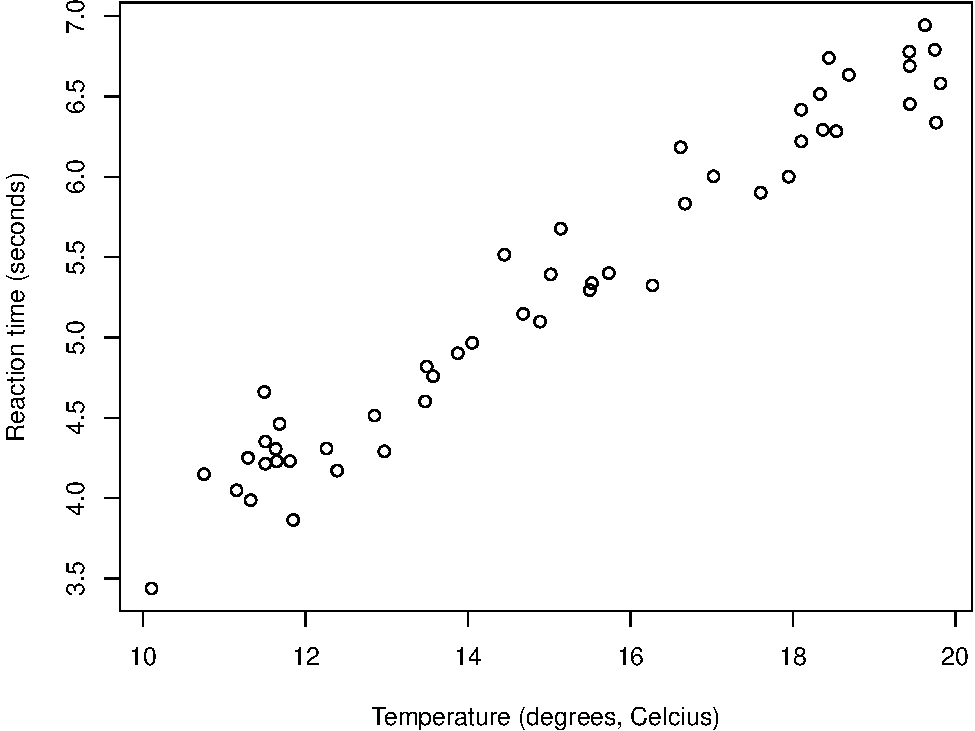
\includegraphics[width=0.8\linewidth]{ECOMODbook_files/figure-latex/Freg-1} 

}

\caption{An example regression data set that could be eplained by a linear regression}\label{fig:Freg}
\end{figure}

It seems like there is a linear relationship between the predictor (temperature) and the response (the reaction time). We could therepore model it with a simple linear regression. We can do that using R´s function \texttt{lm}. We do so here and then look at the summary of the object produced.

The required argument for \texttt{lm} is the \texttt{formula} that defines the regression model. The symbol \texttt{\textasciitilde{}}is used to represent ``as a function of''. So here we will want something like ``reaction time \textasciitilde{} water temperature''.

While this might seem like a detail, it is a good policy to always fit models using explicitly the \texttt{data} argument, instead of fitting the model to objects hanging around the workspace. Learn how to be tidy!

Therefore, while the imideate result would be the same, we suggest that you do not do this

\begin{Shaded}
\begin{Highlighting}[]
\NormalTok{mod0<-}\KeywordTok{lm}\NormalTok{(react}\OperatorTok{~}\NormalTok{temp)}
\end{Highlighting}
\end{Shaded}

nor this

\begin{Shaded}
\begin{Highlighting}[]
\NormalTok{mod0<-}\KeywordTok{lm}\NormalTok{(reaction}\OperatorTok{$}\NormalTok{react}\OperatorTok{~}\NormalTok{reaction}\OperatorTok{$}\NormalTok{temp)}
\end{Highlighting}
\end{Shaded}

but always consider this

\begin{Shaded}
\begin{Highlighting}[]
\NormalTok{mod0<-}\KeywordTok{lm}\NormalTok{(react}\OperatorTok{~}\NormalTok{temp,}\DataTypeTok{data=}\NormalTok{reaction)}
\KeywordTok{summary}\NormalTok{(mod0)}
\end{Highlighting}
\end{Shaded}

\begin{verbatim}
## 
## Call:
## lm(formula = react ~ temp, data = reaction)
## 
## Residuals:
##      Min       1Q   Median       3Q      Max 
## -0.43172 -0.13223 -0.01381  0.13843  0.49265 
## 
## Coefficients:
##             Estimate Std. Error t value Pr(>|t|)    
## (Intercept)  0.55487    0.15642   3.547 0.000881 ***
## temp         0.31442    0.01015  30.986  < 2e-16 ***
## ---
## Signif. codes:  0 '***' 0.001 '**' 0.01 '*' 0.05 '.' 0.1 ' ' 1
## 
## Residual standard error: 0.2182 on 48 degrees of freedom
## Multiple R-squared:  0.9524,	Adjusted R-squared:  0.9514 
## F-statistic: 960.2 on 1 and 48 DF,  p-value: < 2.2e-16
\end{verbatim}

This will be easier to read for others, makes you tidy, and will save you headaches when using functions like \texttt{predict} over the resulting fitted model.

We can the estimated regression line to the above plot. I color it red to remind us of the fact that this is an estimated line, not the true line that generated the data. While in general we do not know this with real data, here I know the model that was used to simulate the data. Just for comparison I can add it to the plot to compare with the estimated regression line.

\begin{Shaded}
\begin{Highlighting}[]
\KeywordTok{plot}\NormalTok{(react}\OperatorTok{~}\NormalTok{temp,}\DataTypeTok{xlab=}\StringTok{"Temperature (degrees, Celcius)"}\NormalTok{,}\DataTypeTok{ylab=}\StringTok{"Reaction time (seconds)"}\NormalTok{)}
\KeywordTok{abline}\NormalTok{(mod0,}\DataTypeTok{lty=}\DecValTok{2}\NormalTok{,}\DataTypeTok{col=}\StringTok{"red"}\NormalTok{)}
\KeywordTok{abline}\NormalTok{(beta0,beta1,}\DataTypeTok{lty=}\DecValTok{2}\NormalTok{,}\DataTypeTok{col=}\StringTok{"green"}\NormalTok{)}
\KeywordTok{legend}\NormalTok{(}\StringTok{"topleft"}\NormalTok{,}\DataTypeTok{legend=}\KeywordTok{c}\NormalTok{(}\StringTok{"Real model"}\NormalTok{,}\StringTok{"Estimated Regression Line"}\NormalTok{),}\DataTypeTok{col=}\KeywordTok{c}\NormalTok{(}\StringTok{"green"}\NormalTok{,}\StringTok{"red"}\NormalTok{),}\DataTypeTok{lty=}\DecValTok{2}\NormalTok{, }\DataTypeTok{inset=}\FloatTok{0.05}\NormalTok{)}
\end{Highlighting}
\end{Shaded}

\includegraphics{ECOMODbook_files/figure-latex/unnamed-chunk-5-1.pdf}

The estimated line and the true line are very similar, as expected since we have a reasonable sample size, a small error, and a model that is the reality. With real data, this will be the exception, not the rule. All models are wrong, but some are useful. The linear regression model is perhaps one of the simplest, but also one of the most widely used, and hence, one of those that has been extremely useful. But of course, its simplicity is also its major disadvantage, as we shall see.

\hypertarget{the-assumptions-are-on-the-residuals-not-the-data}{%
\section{The assumptions are on the residuals, not the data}\label{the-assumptions-are-on-the-residuals-not-the-data}}

Imagine that you have a single variable that you are interested in modelling. This is the concentration of an enzime in the blood of small rodents, from 4 diffferent species. This is represented in the image below \ref{fig:figrodents}.

\begin{Shaded}
\begin{Highlighting}[]
\KeywordTok{hist}\NormalTok{(ys,}\DataTypeTok{breaks=}\DecValTok{0}\OperatorTok{:}\DecValTok{40}\NormalTok{,}\DataTypeTok{xlab=}\StringTok{"Concentration of enzime (mg/L)"}\NormalTok{)}
\end{Highlighting}
\end{Shaded}

\begin{figure}

{\centering 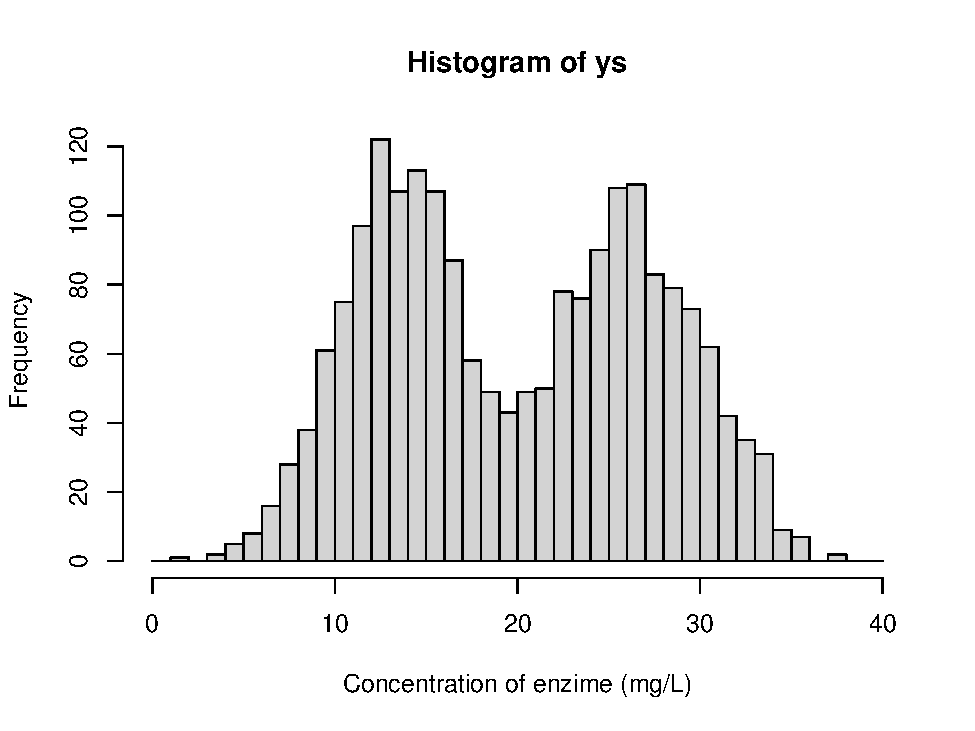
\includegraphics[width=0.8\linewidth]{ECOMODbook_files/figure-latex/figrodents-1} 

}

\caption{Concentration of an enzime (mg/L) in the blood of small rodents, from 4 diffferent species}\label{fig:figrodents}
\end{figure}

A poor (conventional and traditional) biologist would die if shown this dataset, but the truth is there would be no reason for it. If one accounts for the different species, this is what we see. Clear differences between two groups of species.

\begin{Shaded}
\begin{Highlighting}[]
\KeywordTok{boxplot}\NormalTok{(ys}\OperatorTok{~}\NormalTok{type,}\DataTypeTok{ylab=}\StringTok{"Concentration of enzime (mg/L)"}\NormalTok{)}
\end{Highlighting}
\end{Shaded}

\includegraphics{ECOMODbook_files/figure-latex/unnamed-chunk-7-1.pdf}

And further, we can see that the remaining residuals are a beautiful Gaussian. Not a surprise, since this was simulated data, from a Gaussian model :) !

\begin{Shaded}
\begin{Highlighting}[]
\KeywordTok{hist}\NormalTok{(}\KeywordTok{residuals}\NormalTok{(}\KeywordTok{lm}\NormalTok{(ys}\OperatorTok{~}\NormalTok{type)),}\DataTypeTok{main=}\StringTok{""}\NormalTok{,}\DataTypeTok{xlab=}\StringTok{"Residuals"}\NormalTok{)}
\end{Highlighting}
\end{Shaded}

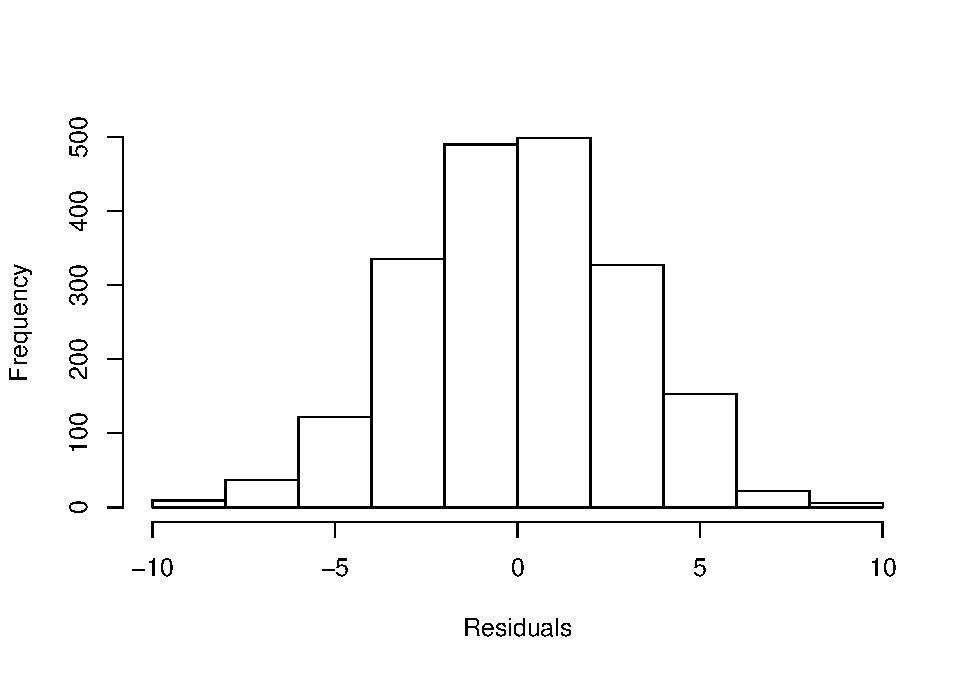
\includegraphics{ECOMODbook_files/figure-latex/unnamed-chunk-8-1.pdf}

The take home message from the story: what the data looks like might be irrelevant. The patterns that remain in the residuals, if any, those are the ones we might need to worry about. So do not transform data just becasue the data looks odd. It might just be Gaussian data in disguise!

\hypertarget{aula6}{%
\chapter{Class 6 13 10 2020}\label{aula6}}

\hypertarget{implementing-a-regression}{%
\section{Implementing a regression}\label{implementing-a-regression}}

We begin by reading the data in ``lagartos.txt'' and fitting a regression model to it.

Read the data in

\begin{Shaded}
\begin{Highlighting}[]
\CommentTok{#folder<-"../Aula6 13 10 2020/"}
\NormalTok{folder<-}\StringTok{"extfiles/"}
\NormalTok{lagartos <-}\StringTok{ }\KeywordTok{read.csv}\NormalTok{(}\DataTypeTok{file=}\KeywordTok{paste0}\NormalTok{(folder,}\StringTok{"lagartos.txt"}\NormalTok{), }\DataTypeTok{sep=}\StringTok{""}\NormalTok{)}
\NormalTok{n <-}\StringTok{ }\KeywordTok{nrow}\NormalTok{(lagartos)}
\end{Highlighting}
\end{Shaded}

We see that we have 97 observations.

Plot the data

\begin{Shaded}
\begin{Highlighting}[]
\KeywordTok{with}\NormalTok{(lagartos,}\KeywordTok{plot}\NormalTok{(peso}\OperatorTok{~}\NormalTok{comp))}
\end{Highlighting}
\end{Shaded}

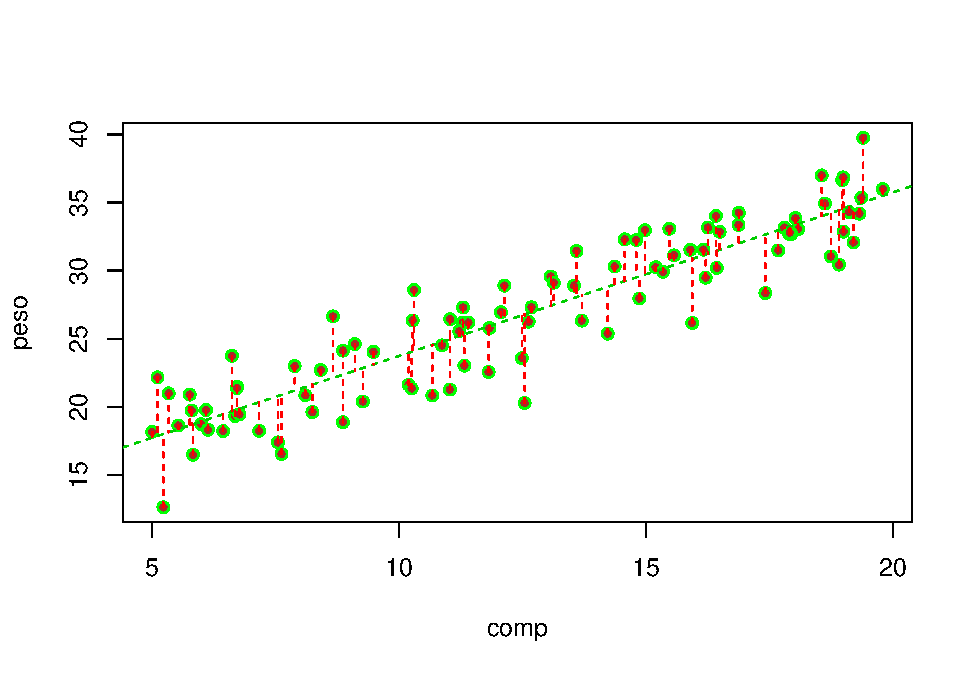
\includegraphics{ECOMODbook_files/figure-latex/unnamed-chunk-10-1.pdf}

A linear model seems adequate. Lets fit a regression line to the data

\begin{Shaded}
\begin{Highlighting}[]
\NormalTok{lmlag <-}\StringTok{ }\KeywordTok{lm}\NormalTok{(peso}\OperatorTok{~}\NormalTok{comp,}\DataTypeTok{data=}\NormalTok{lagartos)}
\KeywordTok{summary}\NormalTok{(lmlag)}
\end{Highlighting}
\end{Shaded}

\begin{verbatim}
## 
## Call:
## lm(formula = peso ~ comp, data = lagartos)
## 
## Residuals:
##     Min      1Q  Median      3Q     Max 
## -6.5199 -1.6961  0.3495  1.7490  4.7127 
## 
## Coefficients:
##             Estimate Std. Error t value Pr(>|t|)    
## (Intercept) 11.72234    0.72299   16.21   <2e-16 ***
## comp         1.20233    0.05402   22.26   <2e-16 ***
## ---
## Signif. codes:  0 '***' 0.001 '**' 0.01 '*' 0.05 '.' 0.1 ' ' 1
## 
## Residual standard error: 2.415 on 95 degrees of freedom
## Multiple R-squared:  0.8391,	Adjusted R-squared:  0.8374 
## F-statistic: 495.3 on 1 and 95 DF,  p-value: < 2.2e-16
\end{verbatim}

Remember that a linear model is just a special GLM:

\begin{Shaded}
\begin{Highlighting}[]
\NormalTok{glmlag <-}\StringTok{ }\KeywordTok{glm}\NormalTok{(peso}\OperatorTok{~}\NormalTok{comp,}\DataTypeTok{data=}\NormalTok{lagartos,}\DataTypeTok{family=}\KeywordTok{gaussian}\NormalTok{(}\DataTypeTok{link=}\StringTok{"identity"}\NormalTok{))}
\KeywordTok{summary}\NormalTok{(glmlag)}
\end{Highlighting}
\end{Shaded}

\begin{verbatim}
## 
## Call:
## glm(formula = peso ~ comp, family = gaussian(link = "identity"), 
##     data = lagartos)
## 
## Deviance Residuals: 
##     Min       1Q   Median       3Q      Max  
## -6.5199  -1.6961   0.3495   1.7490   4.7127  
## 
## Coefficients:
##             Estimate Std. Error t value Pr(>|t|)    
## (Intercept) 11.72234    0.72299   16.21   <2e-16 ***
## comp         1.20233    0.05402   22.26   <2e-16 ***
## ---
## Signif. codes:  0 '***' 0.001 '**' 0.01 '*' 0.05 '.' 0.1 ' ' 1
## 
## (Dispersion parameter for gaussian family taken to be 5.830492)
## 
##     Null deviance: 3441.8  on 96  degrees of freedom
## Residual deviance:  553.9  on 95  degrees of freedom
## AIC: 450.27
## 
## Number of Fisher Scoring iterations: 2
\end{verbatim}

as we can see the output looks a bit different (after all, \texttt{lm} and \texttt{glm} are different functions!), but the results are exactly the same. This does not prove it, but it illustrates by example that a lm is just a GLM with a Gaussian response and an \texttt{identity} link function.

Lets use the results from \texttt{lm}, while noting that everything else would be the same.

The estimated regression line is

peso =11.72 +1.2 \(\times\) comp

and the estimated R-squared is 0.84. The standard error associated with the model is estimated to be 2.4146. Below we explain what each of these values correspond to.

The estimated standard error corresponds to the standard deviation of the residuals of the model, that is, the diference between the observations and the predicted values given the model.

The observation we have already, those are the \texttt{peso}. We can obtain the predicted \texttt{peso} for each observation with the function \texttt{predict}, but here we do it manually so that we see that the errors are just the observations minus the predictions.

\begin{Shaded}
\begin{Highlighting}[]
\CommentTok{#get estimated values}
\NormalTok{estimated<-}\KeywordTok{with}\NormalTok{(lagartos,}\KeywordTok{summary}\NormalTok{(lmlag)}\OperatorTok{$}\NormalTok{coefficients[}\DecValTok{1}\NormalTok{]}\OperatorTok{+}\KeywordTok{summary}\NormalTok{(lmlag)}\OperatorTok{$}\NormalTok{coefficients[}\DecValTok{2}\NormalTok{]}\OperatorTok{*}\NormalTok{comp)}
\CommentTok{# note this would be the same as}
\CommentTok{# estimated<-predict(lmlag)}
\end{Highlighting}
\end{Shaded}

Now we can compute the residuals and their corresponding standard error

\begin{Shaded}
\begin{Highlighting}[]
\CommentTok{#get residuals}
\CommentTok{#erros = observações - valores previstos}
\CommentTok{# e= y- (a+bx)}
\CommentTok{# y= (a+bx) + e}
\NormalTok{resid<-lagartos}\OperatorTok{$}\NormalTok{peso}\OperatorTok{-}\NormalTok{estimated}
\KeywordTok{sd}\NormalTok{(resid)}
\end{Highlighting}
\end{Shaded}

\begin{verbatim}
## [1] 2.402032
\end{verbatim}

Note as predict, we could use just the function \texttt{residuals} with the model object as argument to get us the residuals in a single line of code.

The reason the above standard error is not exactly the same as in the model output above has to do with the degrees of freedom, a concepth that is hard to explain in this applied context, but relates to the number of available independent bits of information available. So turst me when I say that we loose a degree of freedom for each parameter estimated in a model. The exact value of the standard deviation as estimated in the model must account for that loss of one extra degree of freedom (associated with estimating the slope of the line), and so the standard formula of the \texttt{sd} needs to be adjusted for the lost degree of freedom, like this:

\begin{Shaded}
\begin{Highlighting}[]
\CommentTok{#Residual Standard error (Like Standard Deviation)}
\CommentTok{#the right way}
\CommentTok{#Subtract one to ignore intercept}
\NormalTok{k=}\KeywordTok{length}\NormalTok{(lmlag}\OperatorTok{$}\NormalTok{coefficients)}\OperatorTok{-}\DecValTok{1} 
\CommentTok{#get the error sum of squares}
\NormalTok{SSE=}\KeywordTok{sum}\NormalTok{(lmlag}\OperatorTok{$}\NormalTok{residuals}\OperatorTok{**}\DecValTok{2}\NormalTok{)}
\CommentTok{#Residual Standard Error}
\KeywordTok{sqrt}\NormalTok{(SSE}\OperatorTok{/}\NormalTok{(n}\OperatorTok{-}\NormalTok{(}\DecValTok{1}\OperatorTok{+}\NormalTok{k))) }
\end{Highlighting}
\end{Shaded}

\begin{verbatim}
## [1] 2.414641
\end{verbatim}

\begin{Shaded}
\begin{Highlighting}[]
\CommentTok{#equivalently}
\KeywordTok{sqrt}\NormalTok{(}\KeywordTok{var}\NormalTok{(resid)}\OperatorTok{*}\NormalTok{(n}\DecValTok{-1}\NormalTok{)}\OperatorTok{/}\NormalTok{(n}\DecValTok{-2}\NormalTok{))}
\end{Highlighting}
\end{Shaded}

\begin{verbatim}
## [1] 2.414641
\end{verbatim}

Now we get the exact same value as above: 2.4146412.

The \texttt{summary} of the model above is very useful, but nothing like adding the estimated model to the plot with the data. We can easily add the line to the plot with function \texttt{abline} (tip: note the ab in \texttt{abline} correspond to the \(a\) and \(b\) in \(y=a+bx\), but the function abline is ``smart'' enough to take an object of class \texttt{lm} and extract the corresponding \(a\) and \(b\) for plotting)

\begin{Shaded}
\begin{Highlighting}[]
\CommentTok{#with(lagartos,plot(peso~comp))}
\KeywordTok{plot}\NormalTok{(peso}\OperatorTok{~}\NormalTok{comp,}\DataTypeTok{data=}\NormalTok{lagartos)}
\CommentTok{#these next 3 lines are equivalent}
\KeywordTok{abline}\NormalTok{(lmlag,}\DataTypeTok{col=}\StringTok{"orange"}\NormalTok{)}
\KeywordTok{abline}\NormalTok{(}\DataTypeTok{a=}\FloatTok{11.72234}\NormalTok{,}\DataTypeTok{b=}\FloatTok{1.20233}\NormalTok{,}\DataTypeTok{col=}\StringTok{"pink"}\NormalTok{)}
\CommentTok{# y = a + bx}
\KeywordTok{abline}\NormalTok{(}\DataTypeTok{a=}\KeywordTok{summary}\NormalTok{(lmlag)}\OperatorTok{$}\NormalTok{coefficients[}\DecValTok{1}\NormalTok{,}\DecValTok{1}\NormalTok{],}\DataTypeTok{b=}\KeywordTok{summary}\NormalTok{(lmlag)}\OperatorTok{$}\NormalTok{coefficients[}\DecValTok{2}\NormalTok{,}\DecValTok{1}\NormalTok{],}\DataTypeTok{col=}\StringTok{"brown"}\NormalTok{)}
\end{Highlighting}
\end{Shaded}

\includegraphics{ECOMODbook_files/figure-latex/unnamed-chunk-16-1.pdf}

Note the last line works because the parameter estimates are hold in a component of the \texttt{summary} of the fitted model called \texttt{coefficients}

\begin{Shaded}
\begin{Highlighting}[]
\KeywordTok{summary}\NormalTok{(lmlag)}\OperatorTok{$}\NormalTok{coefficients}
\end{Highlighting}
\end{Shaded}

\begin{verbatim}
##              Estimate Std. Error  t value     Pr(>|t|)
## (Intercept) 11.722343 0.72299153 16.21367 4.135172e-29
## comp         1.202333 0.05402397 22.25555 1.839784e-39
\end{verbatim}

Additionally, we can also add the residuals in the plot (we use the very handy function \texttt{segments}, that adds segments to plots, to do so)

\begin{Shaded}
\begin{Highlighting}[]
\CommentTok{# get estimated/predicted values with function residuals}
\NormalTok{estimated2<-}\KeywordTok{predict}\NormalTok{(lmlag)}
\CommentTok{#plot the data}
\KeywordTok{with}\NormalTok{(lagartos,}\KeywordTok{plot}\NormalTok{(peso}\OperatorTok{~}\NormalTok{comp,}\DataTypeTok{pch=}\DecValTok{21}\NormalTok{,}\DataTypeTok{bg=}\StringTok{"brown"}\NormalTok{,}\DataTypeTok{col=}\StringTok{"green"}\NormalTok{))}
\KeywordTok{abline}\NormalTok{(lmlag,}\DataTypeTok{col=}\DecValTok{3}\NormalTok{,}\DataTypeTok{lty=}\DecValTok{2}\NormalTok{)}
\CommentTok{#add residuals}
\KeywordTok{with}\NormalTok{(lagartos,}\KeywordTok{segments}\NormalTok{(}\DataTypeTok{x0 =}\NormalTok{ comp,}\DataTypeTok{y0 =}\NormalTok{ peso, }\DataTypeTok{x1=}\NormalTok{ comp, }\DataTypeTok{y1=}\NormalTok{estimated,}\DataTypeTok{lty=}\DecValTok{2}\NormalTok{,}\DataTypeTok{col=}\StringTok{"red"}\NormalTok{))}
\end{Highlighting}
\end{Shaded}

\includegraphics{ECOMODbook_files/figure-latex/unnamed-chunk-18-1.pdf}

The regression line is the line that minimizes the sum of the red distances in the plot above. That is also why it is called a minimum squares estimate in the special case of a Gaussian model (in PT, é a reta dos mínimos quadrados).

The residuals should, if the model is reasonable - and here that should be the case - be well approximated by a Gaussian distribution. Note we can get the values of the residuals by the difference between the observations and the estimated values, as we did above. We can look at their histogram below

\begin{Shaded}
\begin{Highlighting}[]
\KeywordTok{hist}\NormalTok{(resid,}\DataTypeTok{main=}\StringTok{"Residuals by hand"}\NormalTok{,}\DataTypeTok{freq=}\OtherTok{FALSE}\NormalTok{)}
\CommentTok{#adding the theorethical density of a Gaussian with mean 0 and the}
\CommentTok{#correct standard error}
\KeywordTok{lines}\NormalTok{(}\KeywordTok{seq}\NormalTok{(}\OperatorTok{-}\DecValTok{8}\NormalTok{,}\DecValTok{8}\NormalTok{,}\DataTypeTok{by=}\FloatTok{0.1}\NormalTok{),}\KeywordTok{dnorm}\NormalTok{(}\KeywordTok{seq}\NormalTok{(}\OperatorTok{-}\DecValTok{8}\NormalTok{,}\DecValTok{8}\NormalTok{,}\DataTypeTok{by=}\FloatTok{0.1}\NormalTok{),}\DataTypeTok{mean=}\DecValTok{0}\NormalTok{,}\DataTypeTok{sd=}\KeywordTok{summary}\NormalTok{(lmlag)}\OperatorTok{$}\NormalTok{sigma))}
\end{Highlighting}
\end{Shaded}

\includegraphics{ECOMODbook_files/figure-latex/unnamed-chunk-19-1.pdf}

or alternatively we can use the bespoke function \texttt{residuals}

\begin{Shaded}
\begin{Highlighting}[]
\NormalTok{resid2<-}\KeywordTok{residuals}\NormalTok{(lmlag)}
\KeywordTok{hist}\NormalTok{(resid2,}\DataTypeTok{main=}\StringTok{"Residuals by function residuals"}\NormalTok{)}
\end{Highlighting}
\end{Shaded}

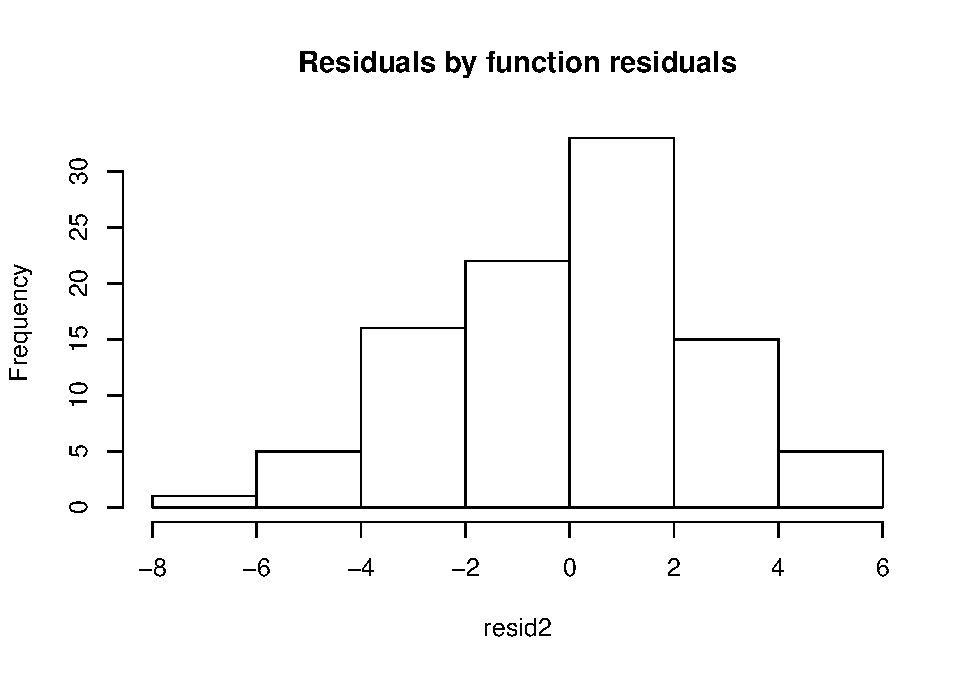
\includegraphics{ECOMODbook_files/figure-latex/unnamed-chunk-20-1.pdf}

It is often said that the \(R^2\) represents the amount of variation in the response that the regression explains. Why is that?

Because if you assume that all the variability in the response data, the \(y_i\) the diference between the data points and a common mean

\[\sum_{i=1}^n (y_i- \bar y)^2\]

in an image, the sum of the square of these quantities

\begin{Shaded}
\begin{Highlighting}[]
\CommentTok{#plot}
\KeywordTok{with}\NormalTok{(lagartos,}\KeywordTok{plot}\NormalTok{(peso}\OperatorTok{~}\NormalTok{comp))}
\KeywordTok{abline}\NormalTok{(lmlag,}\DataTypeTok{col=}\DecValTok{3}\NormalTok{,}\DataTypeTok{lty=}\DecValTok{2}\NormalTok{)}
\KeywordTok{abline}\NormalTok{(}\DataTypeTok{h=}\KeywordTok{mean}\NormalTok{(lagartos}\OperatorTok{$}\NormalTok{peso))}
\KeywordTok{with}\NormalTok{(lagartos,}\KeywordTok{segments}\NormalTok{(}\DataTypeTok{x0 =}\NormalTok{ comp,}\DataTypeTok{y0 =}\NormalTok{ peso, }\DataTypeTok{x1=}\NormalTok{ comp, }\DataTypeTok{y1=}\KeywordTok{mean}\NormalTok{(peso),}\DataTypeTok{lty=}\DecValTok{2}\NormalTok{,}\DataTypeTok{col=}\DecValTok{2}\NormalTok{))}
\end{Highlighting}
\end{Shaded}

\includegraphics{ECOMODbook_files/figure-latex/unnamed-chunk-21-1.pdf}

\begin{Shaded}
\begin{Highlighting}[]
\NormalTok{all.var<-}\KeywordTok{sum}\NormalTok{((lagartos}\OperatorTok{$}\NormalTok{peso}\OperatorTok{-}\KeywordTok{mean}\NormalTok{(lagartos}\OperatorTok{$}\NormalTok{peso))}\OperatorTok{^}\DecValTok{2}\NormalTok{)}
\NormalTok{all.var}
\end{Highlighting}
\end{Shaded}

\begin{verbatim}
## [1] 3441.795
\end{verbatim}

and the variability that is not explained is the one that remains in the errors (the corresponding plot was shown above)

\[\sum_{i=1}^n (y_i- \hat y_i)^2\]

\begin{Shaded}
\begin{Highlighting}[]
\NormalTok{error.var<-}\KeywordTok{sum}\NormalTok{((lagartos}\OperatorTok{$}\NormalTok{peso}\OperatorTok{-}\NormalTok{estimated)}\OperatorTok{^}\DecValTok{2}\NormalTok{)}
\NormalTok{error.var}
\end{Highlighting}
\end{Shaded}

\begin{verbatim}
## [1] 553.8968
\end{verbatim}

then the ratio of those two quantities is what is NOT explained by the regression model, and therefore, 1 minus that is what explained by the regression model.

\begin{Shaded}
\begin{Highlighting}[]
\DecValTok{1}\OperatorTok{-}\NormalTok{error.var}\OperatorTok{/}\NormalTok{all.var}
\end{Highlighting}
\end{Shaded}

\begin{verbatim}
## [1] 0.8390675
\end{verbatim}

And that\ldots{} as noted above\ldots{} is the \(R^2\)=0.8391. This comes from the fact that all of the variability in the data (the \(y\), the response, here the \texttt{peso}) can be decomposed into the variability explained by the model, and the unexplained variability, that of the errors. In a formula

\[SS_{TOTAL}=SS_{REGRESSÃO}+SS_{ERRO}\]

Note naturally we could also represent in an image what is explained by the regression model, which is

\[\sum_{i=1}^n (\hat y_i- \bar y)^2\]

\begin{Shaded}
\begin{Highlighting}[]
\CommentTok{#plot}
\KeywordTok{with}\NormalTok{(lagartos,}\KeywordTok{plot}\NormalTok{(peso}\OperatorTok{~}\NormalTok{comp))}
\KeywordTok{abline}\NormalTok{(lmlag,}\DataTypeTok{col=}\DecValTok{3}\NormalTok{,}\DataTypeTok{lty=}\DecValTok{2}\NormalTok{)}
\KeywordTok{abline}\NormalTok{(}\DataTypeTok{h=}\KeywordTok{mean}\NormalTok{(lagartos}\OperatorTok{$}\NormalTok{peso))}
\KeywordTok{with}\NormalTok{(lagartos,}\KeywordTok{segments}\NormalTok{(}\DataTypeTok{x0 =}\NormalTok{ comp,}\DataTypeTok{y0 =}\NormalTok{ estimated, }\DataTypeTok{x1=}\NormalTok{ comp, }\DataTypeTok{y1=}\KeywordTok{mean}\NormalTok{(peso),}\DataTypeTok{lty=}\DecValTok{2}\NormalTok{,}\DataTypeTok{col=}\DecValTok{2}\NormalTok{))}
\end{Highlighting}
\end{Shaded}

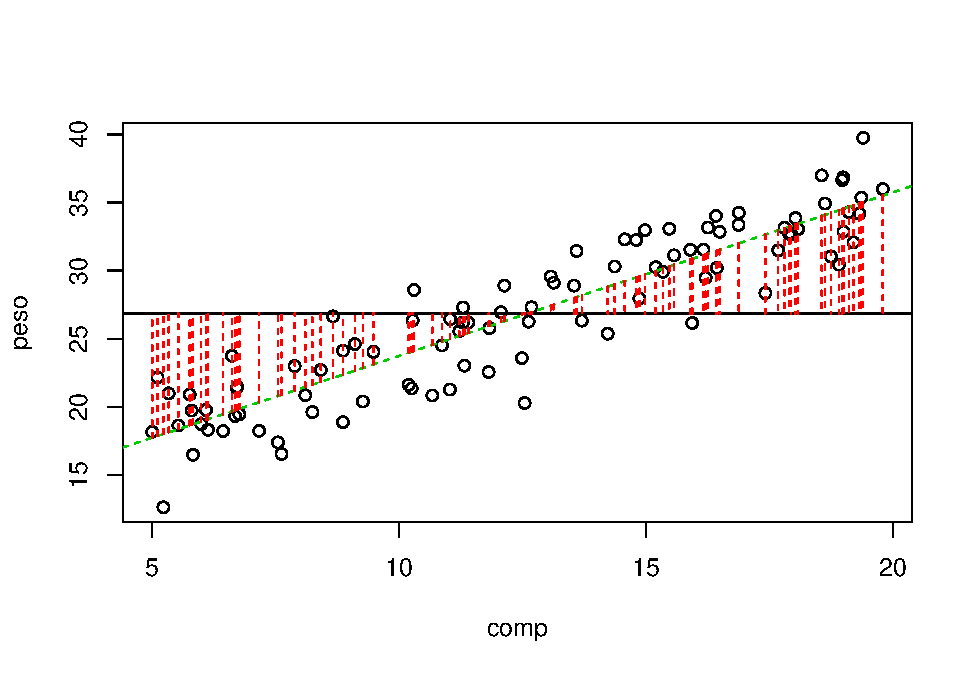
\includegraphics{ECOMODbook_files/figure-latex/unnamed-chunk-25-1.pdf}

and that naturally is obtained as

\begin{Shaded}
\begin{Highlighting}[]
\NormalTok{reg.var<-}\KeywordTok{sum}\NormalTok{((}\KeywordTok{mean}\NormalTok{(lagartos}\OperatorTok{$}\NormalTok{peso)}\OperatorTok{-}\NormalTok{estimated)}\OperatorTok{^}\DecValTok{2}\NormalTok{)}
\NormalTok{reg.var}
\end{Highlighting}
\end{Shaded}

\begin{verbatim}
## [1] 2887.898
\end{verbatim}

and hence the total variability is given by the sum \(SS_{REGRESSÃO}+SS_{ERRO}\)

\begin{Shaded}
\begin{Highlighting}[]
\NormalTok{reg.var}\OperatorTok{+}\NormalTok{error.var}
\end{Highlighting}
\end{Shaded}

\begin{verbatim}
## [1] 3441.795
\end{verbatim}

\begin{Shaded}
\begin{Highlighting}[]
\NormalTok{all.var}
\end{Highlighting}
\end{Shaded}

\begin{verbatim}
## [1] 3441.795
\end{verbatim}

So, always remember that

\[SS_{TOTAL}=SS_{REGRESSÃO}+SS_{ERRO}\]

This is also something that comes out often in books without a clear explanation of the reaon why that holds. While here I show it by example, it could be easily demonstrated algebraically if one wanted that

\[\sum_{i=1}^n (y_i- \bar y)^2=\sum_{i=1}^n (\hat y_i- \bar y)^2 + \sum_{i=1}^n (y_i- \hat y_i)^2\]

If you want that, this 28 minute video shows you the proof: \url{https://www.youtube.com/watch?v=aQ32qTjqqJM}
I think it could take just 5 minutes ;) but many thanks to Dmitry Leiderman for having it out there! He does it in the context of ANOVA, but ANOVA is just a special case of regression, were you have a continous response and a single categorical explanatory variable. Therefore, have fun !

\hypertarget{simulating-regression-data}{%
\section{Simulating regression data}\label{simulating-regression-data}}

Using the above, simulate data assuming that the TRUE relation between the weight and length of a lizzard was given by

\[ peso = 12 + 1.2 * comp \]

We consider that the usual length of a lizard can be between 5 and 20 cm, and the standard error is 4.

As in the data we will have 97 lizards

Then you were told to create the lengths:

\begin{Shaded}
\begin{Highlighting}[]
\KeywordTok{set.seed}\NormalTok{(}\DecValTok{121}\NormalTok{)}
\NormalTok{n=}\DecValTok{97}
\CommentTok{#lengths}
\NormalTok{xs=}\KeywordTok{runif}\NormalTok{(n,}\DecValTok{5}\NormalTok{,}\DecValTok{20}\NormalTok{)}
\KeywordTok{hist}\NormalTok{(xs,}\DataTypeTok{main=}\StringTok{"Lenths (cm)"}\NormalTok{)}
\end{Highlighting}
\end{Shaded}

\includegraphics{ECOMODbook_files/figure-latex/unnamed-chunk-28-1.pdf}

and then to create weights of lizards

\begin{Shaded}
\begin{Highlighting}[]
\NormalTok{a=}\DecValTok{12}
\NormalTok{b=}\FloatTok{1.2}
\NormalTok{ys=a}\OperatorTok{+}\NormalTok{b}\OperatorTok{*}\NormalTok{xs}
\end{Highlighting}
\end{Shaded}

If we plot the data, all points are in a single line. Why, because there is no randomness.

\begin{Shaded}
\begin{Highlighting}[]
\KeywordTok{plot}\NormalTok{(xs,ys)}
\end{Highlighting}
\end{Shaded}

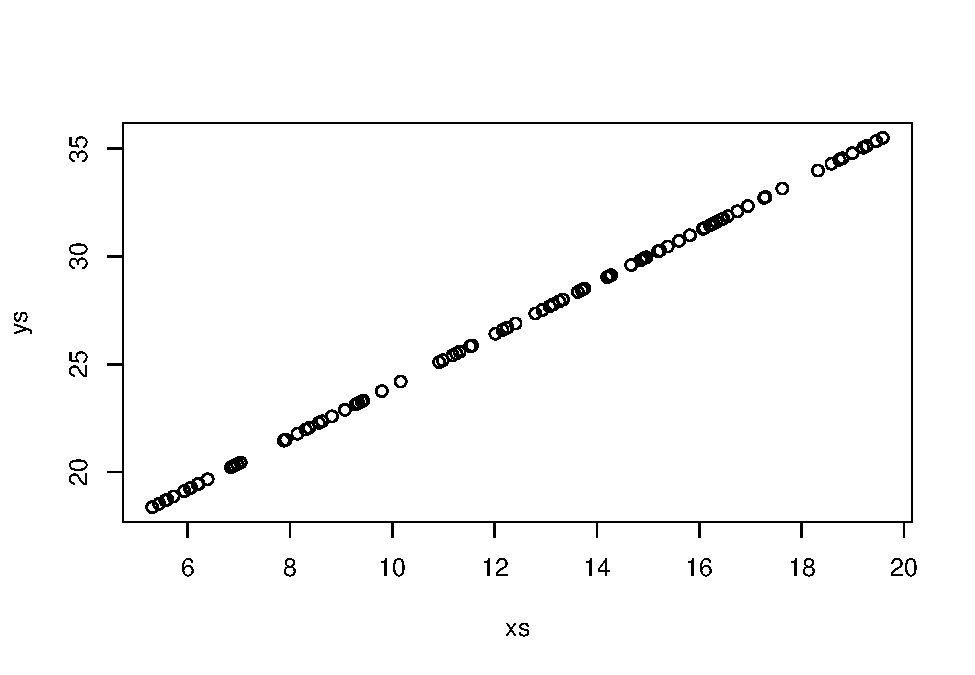
\includegraphics{ECOMODbook_files/figure-latex/unnamed-chunk-30-1.pdf}

This means that if you try to run a model, it gives you a warning that the model might be unreliable

\begin{Shaded}
\begin{Highlighting}[]
\KeywordTok{summary}\NormalTok{(}\KeywordTok{lm}\NormalTok{(ys}\OperatorTok{~}\NormalTok{xs))}
\end{Highlighting}
\end{Shaded}

\begin{verbatim}
## Warning in summary.lm(lm(ys ~ xs)): essentially perfect fit: summary may be
## unreliable
\end{verbatim}

\begin{verbatim}
## 
## Call:
## lm(formula = ys ~ xs)
## 
## Residuals:
##        Min         1Q     Median         3Q        Max 
## -5.595e-15 -2.460e-15 -1.878e-15 -1.422e-15  1.873e-13 
## 
## Coefficients:
##              Estimate Std. Error   t value Pr(>|t|)    
## (Intercept) 1.200e+01  6.050e-15 1.983e+15   <2e-16 ***
## xs          1.200e+00  4.611e-16 2.603e+15   <2e-16 ***
## ---
## Signif. codes:  0 '***' 0.001 '**' 0.01 '*' 0.05 '.' 0.1 ' ' 1
## 
## Residual standard error: 1.934e-14 on 95 degrees of freedom
## Multiple R-squared:      1,	Adjusted R-squared:      1 
## F-statistic: 6.773e+30 on 1 and 95 DF,  p-value: < 2.2e-16
\end{verbatim}

So\ldots{} , we add some variance, and plot the data:

\begin{Shaded}
\begin{Highlighting}[]
\NormalTok{ys=a}\OperatorTok{+}\NormalTok{b}\OperatorTok{*}\NormalTok{xs}\OperatorTok{+}\KeywordTok{rnorm}\NormalTok{(n,}\DecValTok{0}\NormalTok{,}\DecValTok{4}\NormalTok{)}
\KeywordTok{plot}\NormalTok{(xs,ys)}
\end{Highlighting}
\end{Shaded}

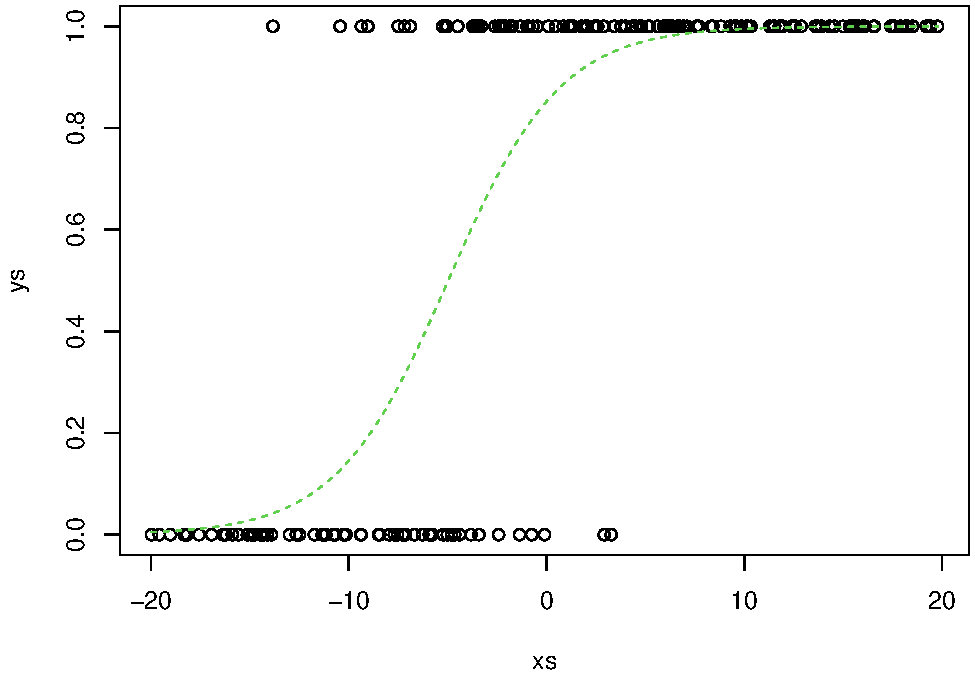
\includegraphics{ECOMODbook_files/figure-latex/unnamed-chunk-32-1.pdf}

Using the code above, experiment with changing the standard deviation of the error, and see what happens to the estimated \(R^2\), to the parameter estimates, to the estimated error, and to how close the estimated regression mode is to the true model (note this is the amazing advantage of a simulation, which we do not have in real data, we know what reality is, and a true model exists!). This will give you a good feeling for what a regression model is and what is does, and what it can't do. An example of what it can't give you is reliable estimates when the error is large compared to the systematic part of the model.

\begin{Shaded}
\begin{Highlighting}[]
\NormalTok{n <-}\StringTok{ }\DecValTok{97}
\CommentTok{#simular comprimentos}
\NormalTok{comp.sim <-}\StringTok{ }\KeywordTok{runif}\NormalTok{(n,}\DecValTok{5}\NormalTok{,}\DecValTok{20}\NormalTok{)}
\NormalTok{a<-}\DecValTok{12}
\NormalTok{b<-}\FloatTok{1.2}
\CommentTok{#simular pesos}
\NormalTok{peso.sim<-a}\OperatorTok{+}\NormalTok{b}\OperatorTok{*}\NormalTok{comp.sim}\OperatorTok{+}\KeywordTok{rnorm}\NormalTok{(n,}\DataTypeTok{mean=}\DecValTok{0}\NormalTok{,}\DataTypeTok{sd=}\DecValTok{2}\NormalTok{)}
\NormalTok{data.sim=}\KeywordTok{data.frame}\NormalTok{(}\DataTypeTok{csim=}\NormalTok{comp.sim,}\DataTypeTok{psim=}\NormalTok{peso.sim)}
\KeywordTok{plot}\NormalTok{(psim}\OperatorTok{~}\NormalTok{csim,}\DataTypeTok{data=}\NormalTok{data.sim)}
\NormalTok{mod.sim<-}\KeywordTok{lm}\NormalTok{(psim}\OperatorTok{~}\NormalTok{csim,}\DataTypeTok{data=}\NormalTok{data.sim)}
\KeywordTok{abline}\NormalTok{(mod.sim,}\DataTypeTok{col=}\StringTok{"red"}\NormalTok{)}
\KeywordTok{summary}\NormalTok{(mod.sim)}
\end{Highlighting}
\end{Shaded}

\begin{verbatim}
## 
## Call:
## lm(formula = psim ~ csim, data = data.sim)
## 
## Residuals:
##     Min      1Q  Median      3Q     Max 
## -5.3460 -1.1652  0.1329  1.5072  3.0036 
## 
## Coefficients:
##             Estimate Std. Error t value Pr(>|t|)    
## (Intercept) 11.70390    0.56783   20.61   <2e-16 ***
## csim         1.20912    0.04325   27.96   <2e-16 ***
## ---
## Signif. codes:  0 '***' 0.001 '**' 0.01 '*' 0.05 '.' 0.1 ' ' 1
## 
## Residual standard error: 1.822 on 95 degrees of freedom
## Multiple R-squared:  0.8916,	Adjusted R-squared:  0.8905 
## F-statistic: 781.6 on 1 and 95 DF,  p-value: < 2.2e-16
\end{verbatim}

\begin{Shaded}
\begin{Highlighting}[]
\KeywordTok{abline}\NormalTok{(a,b,}\DataTypeTok{col=}\StringTok{"green"}\NormalTok{)}
\KeywordTok{legend}\NormalTok{(}\StringTok{"topleft"}\NormalTok{,}\DataTypeTok{legend=}\KeywordTok{c}\NormalTok{(}\StringTok{"Estimated line"}\NormalTok{,}\StringTok{"True model"}\NormalTok{),}\DataTypeTok{col=}\KeywordTok{c}\NormalTok{(}\StringTok{"red"}\NormalTok{,}\StringTok{"green"}\NormalTok{),}\DataTypeTok{lty=}\DecValTok{1}\NormalTok{,}\DataTypeTok{inset=}\FloatTok{0.05}\NormalTok{)}
\end{Highlighting}
\end{Shaded}

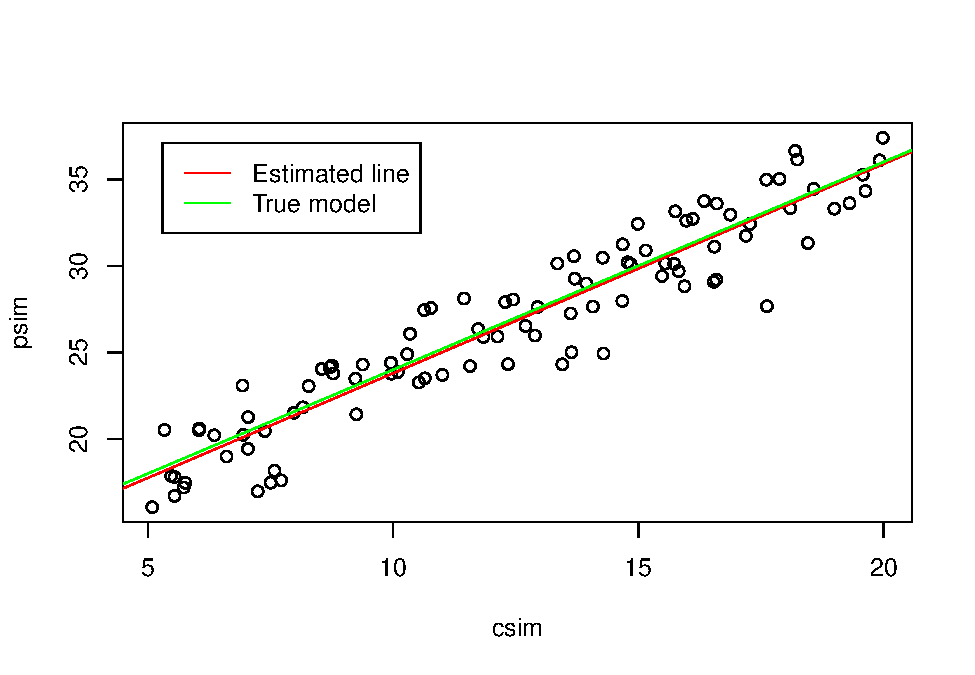
\includegraphics{ECOMODbook_files/figure-latex/unnamed-chunk-33-1.pdf}

\hypertarget{what-is-the-effect-of-increasing-the-error-a-simulation-experiment}{%
\subsection{What is the effect of increasing the error: a simulation experiment}\label{what-is-the-effect-of-increasing-the-error-a-simulation-experiment}}

Now, let's consider there's more and less variance. We also add to each plot the real line (that with the true parameter values) and the one with the estimated parameter values.

\begin{Shaded}
\begin{Highlighting}[]
\KeywordTok{par}\NormalTok{(}\DataTypeTok{mfrow=}\KeywordTok{c}\NormalTok{(}\DecValTok{2}\NormalTok{,}\DecValTok{3}\NormalTok{))}
\NormalTok{ys=a}\OperatorTok{+}\NormalTok{b}\OperatorTok{*}\NormalTok{xs}\OperatorTok{+}\KeywordTok{rnorm}\NormalTok{(n,}\DecValTok{0}\NormalTok{,}\DecValTok{1}\NormalTok{)}
\KeywordTok{plot}\NormalTok{(xs,ys)}
\NormalTok{mod1=}\KeywordTok{lm}\NormalTok{(ys}\OperatorTok{~}\NormalTok{xs)}
\KeywordTok{abline}\NormalTok{(mod1,}\DataTypeTok{col=}\StringTok{"red"}\NormalTok{)}
\KeywordTok{abline}\NormalTok{(a,b,}\DataTypeTok{col=}\StringTok{"green"}\NormalTok{)}
\NormalTok{ys=a}\OperatorTok{+}\NormalTok{b}\OperatorTok{*}\NormalTok{xs}\OperatorTok{+}\KeywordTok{rnorm}\NormalTok{(n,}\DecValTok{0}\NormalTok{,}\DecValTok{2}\NormalTok{)}
\KeywordTok{plot}\NormalTok{(xs,ys)}
\NormalTok{mod2=}\KeywordTok{lm}\NormalTok{(ys}\OperatorTok{~}\NormalTok{xs)}
\KeywordTok{abline}\NormalTok{(mod2,}\DataTypeTok{col=}\StringTok{"red"}\NormalTok{)}
\KeywordTok{abline}\NormalTok{(a,b,}\DataTypeTok{col=}\StringTok{"green"}\NormalTok{)}
\NormalTok{ys=a}\OperatorTok{+}\NormalTok{b}\OperatorTok{*}\NormalTok{xs}\OperatorTok{+}\KeywordTok{rnorm}\NormalTok{(n,}\DecValTok{0}\NormalTok{,}\DecValTok{4}\NormalTok{)}
\KeywordTok{plot}\NormalTok{(xs,ys)}
\NormalTok{mod4=}\KeywordTok{lm}\NormalTok{(ys}\OperatorTok{~}\NormalTok{xs)}
\KeywordTok{abline}\NormalTok{(mod4,}\DataTypeTok{col=}\StringTok{"red"}\NormalTok{)}
\KeywordTok{abline}\NormalTok{(a,b,}\DataTypeTok{col=}\StringTok{"green"}\NormalTok{)}
\NormalTok{ys=a}\OperatorTok{+}\NormalTok{b}\OperatorTok{*}\NormalTok{xs}\OperatorTok{+}\KeywordTok{rnorm}\NormalTok{(n,}\DecValTok{0}\NormalTok{,}\DecValTok{10}\NormalTok{)}
\KeywordTok{plot}\NormalTok{(xs,ys)}
\NormalTok{mod10=}\KeywordTok{lm}\NormalTok{(ys}\OperatorTok{~}\NormalTok{xs)}
\KeywordTok{abline}\NormalTok{(mod10,}\DataTypeTok{col=}\StringTok{"red"}\NormalTok{)}
\KeywordTok{abline}\NormalTok{(a,b,}\DataTypeTok{col=}\StringTok{"green"}\NormalTok{)}
\NormalTok{ys=a}\OperatorTok{+}\NormalTok{b}\OperatorTok{*}\NormalTok{xs}\OperatorTok{+}\KeywordTok{rnorm}\NormalTok{(n,}\DecValTok{0}\NormalTok{,}\DecValTok{20}\NormalTok{)}
\KeywordTok{plot}\NormalTok{(xs,ys)}
\NormalTok{mod20=}\KeywordTok{lm}\NormalTok{(ys}\OperatorTok{~}\NormalTok{xs)}
\KeywordTok{abline}\NormalTok{(mod20,}\DataTypeTok{col=}\StringTok{"red"}\NormalTok{)}
\KeywordTok{abline}\NormalTok{(a,b,}\DataTypeTok{col=}\StringTok{"green"}\NormalTok{)}
\NormalTok{ys=a}\OperatorTok{+}\NormalTok{b}\OperatorTok{*}\NormalTok{xs}\OperatorTok{+}\KeywordTok{rnorm}\NormalTok{(n,}\DecValTok{0}\NormalTok{,}\DecValTok{100}\NormalTok{)}
\KeywordTok{plot}\NormalTok{(xs,ys)}
\NormalTok{mod100=}\KeywordTok{lm}\NormalTok{(ys}\OperatorTok{~}\NormalTok{xs)}
\KeywordTok{abline}\NormalTok{(mod100,}\DataTypeTok{col=}\StringTok{"red"}\NormalTok{)}
\KeywordTok{abline}\NormalTok{(a,b,}\DataTypeTok{col=}\StringTok{"green"}\NormalTok{)}
\end{Highlighting}
\end{Shaded}

\includegraphics{ECOMODbook_files/figure-latex/unnamed-chunk-34-1.pdf}

Not surprisingly, as the variance increases, we get data that more and more looks like it is not coming from a real linear process.

You can also look at the model summaries, and there you can see that, in fact, the models become essentially useless as the variance increases! You can see that both from the correlation, but also by the predictions generated from the model (comparing to the truth), and also the significance of the coefficients associated with the regression parameters.

Make no mistake, the reality is always the same, in terms of the fixed part of the model, it's just the variance that increases.

Also, don't get confused, the different green lines might look different, but they are always exactly the same line! You can check that by forcing the y axis to span the same limits.

\begin{Shaded}
\begin{Highlighting}[]
\KeywordTok{par}\NormalTok{(}\DataTypeTok{mfrow=}\KeywordTok{c}\NormalTok{(}\DecValTok{2}\NormalTok{,}\DecValTok{3}\NormalTok{))}
\NormalTok{ys=a}\OperatorTok{+}\NormalTok{b}\OperatorTok{*}\NormalTok{xs}\OperatorTok{+}\KeywordTok{rnorm}\NormalTok{(n,}\DecValTok{0}\NormalTok{,}\DecValTok{1}\NormalTok{)}
\KeywordTok{plot}\NormalTok{(xs,ys,}\DataTypeTok{ylim=}\KeywordTok{c}\NormalTok{(}\OperatorTok{-}\DecValTok{400}\NormalTok{,}\DecValTok{400}\NormalTok{))}
\NormalTok{mod1=}\KeywordTok{lm}\NormalTok{(ys}\OperatorTok{~}\NormalTok{xs)}
\KeywordTok{abline}\NormalTok{(mod1,}\DataTypeTok{col=}\StringTok{"red"}\NormalTok{)}
\KeywordTok{abline}\NormalTok{(a,b,}\DataTypeTok{col=}\StringTok{"green"}\NormalTok{)}
\NormalTok{ys=a}\OperatorTok{+}\NormalTok{b}\OperatorTok{*}\NormalTok{xs}\OperatorTok{+}\KeywordTok{rnorm}\NormalTok{(n,}\DecValTok{0}\NormalTok{,}\DecValTok{2}\NormalTok{)}
\KeywordTok{plot}\NormalTok{(xs,ys,}\DataTypeTok{ylim=}\KeywordTok{c}\NormalTok{(}\OperatorTok{-}\DecValTok{400}\NormalTok{,}\DecValTok{400}\NormalTok{))}
\NormalTok{mod2=}\KeywordTok{lm}\NormalTok{(ys}\OperatorTok{~}\NormalTok{xs)}
\KeywordTok{abline}\NormalTok{(mod2,}\DataTypeTok{col=}\StringTok{"red"}\NormalTok{)}
\KeywordTok{abline}\NormalTok{(a,b,}\DataTypeTok{col=}\StringTok{"green"}\NormalTok{)}
\NormalTok{ys=a}\OperatorTok{+}\NormalTok{b}\OperatorTok{*}\NormalTok{xs}\OperatorTok{+}\KeywordTok{rnorm}\NormalTok{(n,}\DecValTok{0}\NormalTok{,}\DecValTok{4}\NormalTok{)}
\KeywordTok{plot}\NormalTok{(xs,ys,}\DataTypeTok{ylim=}\KeywordTok{c}\NormalTok{(}\OperatorTok{-}\DecValTok{400}\NormalTok{,}\DecValTok{400}\NormalTok{))}
\NormalTok{mod4=}\KeywordTok{lm}\NormalTok{(ys}\OperatorTok{~}\NormalTok{xs)}
\KeywordTok{abline}\NormalTok{(mod4,}\DataTypeTok{col=}\StringTok{"red"}\NormalTok{)}
\KeywordTok{abline}\NormalTok{(a,b,}\DataTypeTok{col=}\StringTok{"green"}\NormalTok{)}
\NormalTok{ys=a}\OperatorTok{+}\NormalTok{b}\OperatorTok{*}\NormalTok{xs}\OperatorTok{+}\KeywordTok{rnorm}\NormalTok{(n,}\DecValTok{0}\NormalTok{,}\DecValTok{10}\NormalTok{)}
\KeywordTok{plot}\NormalTok{(xs,ys,}\DataTypeTok{ylim=}\KeywordTok{c}\NormalTok{(}\OperatorTok{-}\DecValTok{400}\NormalTok{,}\DecValTok{400}\NormalTok{))}
\NormalTok{mod10=}\KeywordTok{lm}\NormalTok{(ys}\OperatorTok{~}\NormalTok{xs)}
\KeywordTok{abline}\NormalTok{(mod10,}\DataTypeTok{col=}\StringTok{"red"}\NormalTok{)}
\KeywordTok{abline}\NormalTok{(a,b,}\DataTypeTok{col=}\StringTok{"green"}\NormalTok{)}
\NormalTok{ys=a}\OperatorTok{+}\NormalTok{b}\OperatorTok{*}\NormalTok{xs}\OperatorTok{+}\KeywordTok{rnorm}\NormalTok{(n,}\DecValTok{0}\NormalTok{,}\DecValTok{20}\NormalTok{)}
\KeywordTok{plot}\NormalTok{(xs,ys,}\DataTypeTok{ylim=}\KeywordTok{c}\NormalTok{(}\OperatorTok{-}\DecValTok{400}\NormalTok{,}\DecValTok{400}\NormalTok{))}
\NormalTok{mod20=}\KeywordTok{lm}\NormalTok{(ys}\OperatorTok{~}\NormalTok{xs)}
\KeywordTok{abline}\NormalTok{(mod20,}\DataTypeTok{col=}\StringTok{"red"}\NormalTok{)}
\KeywordTok{abline}\NormalTok{(a,b,}\DataTypeTok{col=}\StringTok{"green"}\NormalTok{)}
\NormalTok{ys=a}\OperatorTok{+}\NormalTok{b}\OperatorTok{*}\NormalTok{xs}\OperatorTok{+}\KeywordTok{rnorm}\NormalTok{(n,}\DecValTok{0}\NormalTok{,}\DecValTok{100}\NormalTok{)}
\KeywordTok{plot}\NormalTok{(xs,ys,}\DataTypeTok{ylim=}\KeywordTok{c}\NormalTok{(}\OperatorTok{-}\DecValTok{400}\NormalTok{,}\DecValTok{400}\NormalTok{))}
\NormalTok{mod100=}\KeywordTok{lm}\NormalTok{(ys}\OperatorTok{~}\NormalTok{xs)}
\KeywordTok{abline}\NormalTok{(mod100,}\DataTypeTok{col=}\StringTok{"red"}\NormalTok{)}
\KeywordTok{abline}\NormalTok{(a,b,}\DataTypeTok{col=}\StringTok{"green"}\NormalTok{)}
\end{Highlighting}
\end{Shaded}

\includegraphics{ECOMODbook_files/figure-latex/unnamed-chunk-35-1.pdf}

but since then you loose all the ability to look at the actual data in some of the plots, that is not really that useful!

Below I look at the summary of each model. Look at correlations, at the estimated values for the parameters, their corresponding variances and the \(R^2\).

\begin{Shaded}
\begin{Highlighting}[]
\KeywordTok{summary}\NormalTok{(mod1)}
\end{Highlighting}
\end{Shaded}

\begin{verbatim}
## 
## Call:
## lm(formula = ys ~ xs)
## 
## Residuals:
##      Min       1Q   Median       3Q      Max 
## -2.87715 -0.62444  0.03329  0.69103  2.47244 
## 
## Coefficients:
##             Estimate Std. Error t value Pr(>|t|)    
## (Intercept) 12.24930    0.33691   36.36   <2e-16 ***
## xs           1.18596    0.02568   46.19   <2e-16 ***
## ---
## Signif. codes:  0 '***' 0.001 '**' 0.01 '*' 0.05 '.' 0.1 ' ' 1
## 
## Residual standard error: 1.077 on 95 degrees of freedom
## Multiple R-squared:  0.9574,	Adjusted R-squared:  0.9569 
## F-statistic:  2133 on 1 and 95 DF,  p-value: < 2.2e-16
\end{verbatim}

\begin{Shaded}
\begin{Highlighting}[]
\KeywordTok{summary}\NormalTok{(mod2)}
\end{Highlighting}
\end{Shaded}

\begin{verbatim}
## 
## Call:
## lm(formula = ys ~ xs)
## 
## Residuals:
##     Min      1Q  Median      3Q     Max 
## -4.7122 -1.5245 -0.0731  1.5830  4.5457 
## 
## Coefficients:
##             Estimate Std. Error t value Pr(>|t|)    
## (Intercept) 11.22718    0.66606   16.86   <2e-16 ***
## xs           1.26028    0.05076   24.83   <2e-16 ***
## ---
## Signif. codes:  0 '***' 0.001 '**' 0.01 '*' 0.05 '.' 0.1 ' ' 1
## 
## Residual standard error: 2.129 on 95 degrees of freedom
## Multiple R-squared:  0.8665,	Adjusted R-squared:  0.8651 
## F-statistic: 616.4 on 1 and 95 DF,  p-value: < 2.2e-16
\end{verbatim}

\begin{Shaded}
\begin{Highlighting}[]
\KeywordTok{summary}\NormalTok{(mod4)}
\end{Highlighting}
\end{Shaded}

\begin{verbatim}
## 
## Call:
## lm(formula = ys ~ xs)
## 
## Residuals:
##     Min      1Q  Median      3Q     Max 
## -9.8201 -2.6923  0.0809  2.8841 11.1413 
## 
## Coefficients:
##             Estimate Std. Error t value Pr(>|t|)    
## (Intercept) 12.93903    1.26042   10.27   <2e-16 ***
## xs           1.11757    0.09606   11.63   <2e-16 ***
## ---
## Signif. codes:  0 '***' 0.001 '**' 0.01 '*' 0.05 '.' 0.1 ' ' 1
## 
## Residual standard error: 4.028 on 95 degrees of freedom
## Multiple R-squared:  0.5876,	Adjusted R-squared:  0.5833 
## F-statistic: 135.4 on 1 and 95 DF,  p-value: < 2.2e-16
\end{verbatim}

\begin{Shaded}
\begin{Highlighting}[]
\KeywordTok{summary}\NormalTok{(mod10)}
\end{Highlighting}
\end{Shaded}

\begin{verbatim}
## 
## Call:
## lm(formula = ys ~ xs)
## 
## Residuals:
##     Min      1Q  Median      3Q     Max 
## -23.236  -6.053  -2.186   7.375  25.314 
## 
## Coefficients:
##             Estimate Std. Error t value Pr(>|t|)    
## (Intercept)  12.1949     3.0136   4.047 0.000106 ***
## xs            1.2102     0.2297   5.269 8.54e-07 ***
## ---
## Signif. codes:  0 '***' 0.001 '**' 0.01 '*' 0.05 '.' 0.1 ' ' 1
## 
## Residual standard error: 9.632 on 95 degrees of freedom
## Multiple R-squared:  0.2262,	Adjusted R-squared:  0.218 
## F-statistic: 27.76 on 1 and 95 DF,  p-value: 8.541e-07
\end{verbatim}

\begin{Shaded}
\begin{Highlighting}[]
\KeywordTok{summary}\NormalTok{(mod20)}
\end{Highlighting}
\end{Shaded}

\begin{verbatim}
## 
## Call:
## lm(formula = ys ~ xs)
## 
## Residuals:
##     Min      1Q  Median      3Q     Max 
## -48.932 -16.093   1.632  13.610  55.287 
## 
## Coefficients:
##             Estimate Std. Error t value Pr(>|t|)    
## (Intercept)   9.2412     6.4002   1.444 0.152058    
## xs            1.6652     0.4878   3.414 0.000943 ***
## ---
## Signif. codes:  0 '***' 0.001 '**' 0.01 '*' 0.05 '.' 0.1 ' ' 1
## 
## Residual standard error: 20.46 on 95 degrees of freedom
## Multiple R-squared:  0.1093,	Adjusted R-squared:  0.09991 
## F-statistic: 11.66 on 1 and 95 DF,  p-value: 0.0009426
\end{verbatim}

\begin{Shaded}
\begin{Highlighting}[]
\KeywordTok{summary}\NormalTok{(mod100)}
\end{Highlighting}
\end{Shaded}

\begin{verbatim}
## 
## Call:
## lm(formula = ys ~ xs)
## 
## Residuals:
##      Min       1Q   Median       3Q      Max 
## -214.028  -69.887    0.743   60.602  255.109 
## 
## Coefficients:
##             Estimate Std. Error t value Pr(>|t|)
## (Intercept)  41.6496    30.0996   1.384    0.170
## xs           -0.5455     2.2939  -0.238    0.813
## 
## Residual standard error: 96.2 on 95 degrees of freedom
## Multiple R-squared:  0.0005949,	Adjusted R-squared:  -0.009925 
## F-statistic: 0.05655 on 1 and 95 DF,  p-value: 0.8126
\end{verbatim}

As an example, we can plot the \(R^2\) as a function of the variance

\begin{Shaded}
\begin{Highlighting}[]
\KeywordTok{plot}\NormalTok{(}\KeywordTok{c}\NormalTok{(}\DecValTok{1}\NormalTok{,}\DecValTok{2}\NormalTok{,}\DecValTok{4}\NormalTok{,}\DecValTok{10}\NormalTok{,}\DecValTok{20}\NormalTok{,}\DecValTok{100}\NormalTok{),}\KeywordTok{c}\NormalTok{(}\KeywordTok{summary}\NormalTok{(mod1)}\OperatorTok{$}\NormalTok{r.squared,}\KeywordTok{summary}\NormalTok{(mod2)}\OperatorTok{$}\NormalTok{r.squared,}\KeywordTok{summary}\NormalTok{(mod4)}\OperatorTok{$}\NormalTok{r.squared,}\KeywordTok{summary}\NormalTok{(mod10)}\OperatorTok{$}\NormalTok{r.squared,}\KeywordTok{summary}\NormalTok{(mod20)}\OperatorTok{$}\NormalTok{r.squared,}\KeywordTok{summary}\NormalTok{(mod100)}\OperatorTok{$}\NormalTok{r.squared))}
\end{Highlighting}
\end{Shaded}

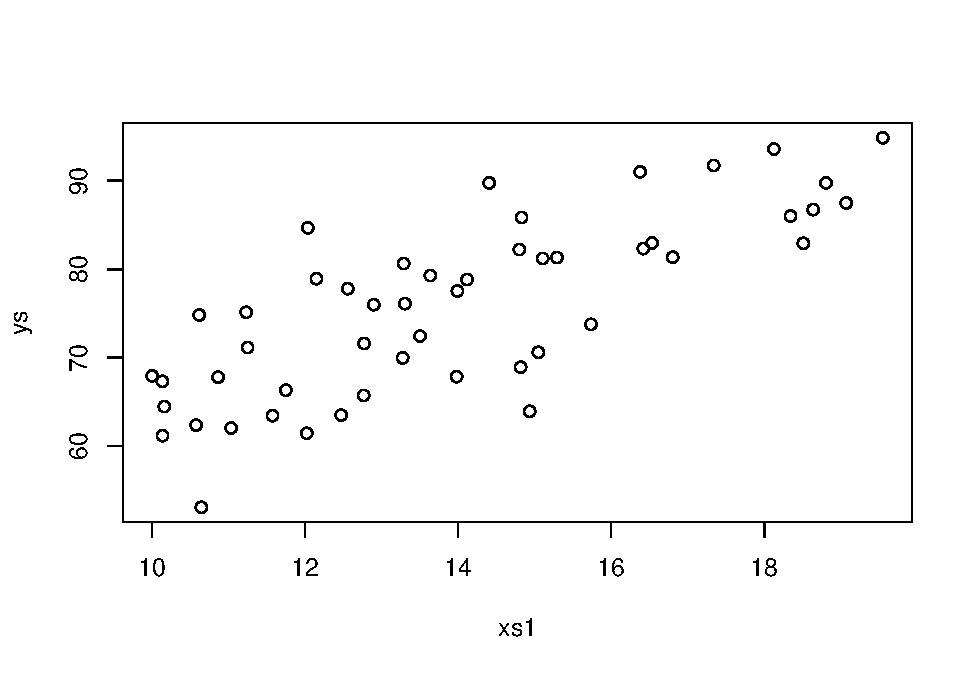
\includegraphics{ECOMODbook_files/figure-latex/unnamed-chunk-37-1.pdf}

That is quite interesting actually\ldots{} There seems to be a nonlinear relationship, but we only have a sample size of six (different standard deviatios, i.e., variances, as variance is standard deviation squared), so hard to tell\ldots{}

Let's show off in R\ldots{}

\begin{Shaded}
\begin{Highlighting}[]
\NormalTok{sds=}\KeywordTok{seq}\NormalTok{(}\FloatTok{0.5}\NormalTok{,}\DecValTok{100}\NormalTok{,}\DataTypeTok{by=}\FloatTok{0.5}\NormalTok{)}
\NormalTok{nsds=}\KeywordTok{length}\NormalTok{(sds)}
\CommentTok{#an object to hold the correlations}
\NormalTok{Rsqs=}\KeywordTok{numeric}\NormalTok{(nsds)}
\ControlFlowTok{for}\NormalTok{ (i }\ControlFlowTok{in} \DecValTok{1}\OperatorTok{:}\NormalTok{nsds)\{}
  \CommentTok{#create data}
\NormalTok{  ys=a}\OperatorTok{+}\NormalTok{b}\OperatorTok{*}\NormalTok{xs}\OperatorTok{+}\KeywordTok{rnorm}\NormalTok{(n,}\DecValTok{0}\NormalTok{,sds[i])}
  \CommentTok{#estimate model}
\NormalTok{  modi=}\KeywordTok{lm}\NormalTok{(ys}\OperatorTok{~}\NormalTok{xs)}
  \CommentTok{#get R-squared}
\NormalTok{  Rsqs[i]=}\KeywordTok{summary}\NormalTok{(modi)}\OperatorTok{$}\NormalTok{r.squared}
\NormalTok{\}}
\CommentTok{#and at the end... plot results}
\KeywordTok{plot}\NormalTok{(sds,Rsqs)}
\end{Highlighting}
\end{Shaded}

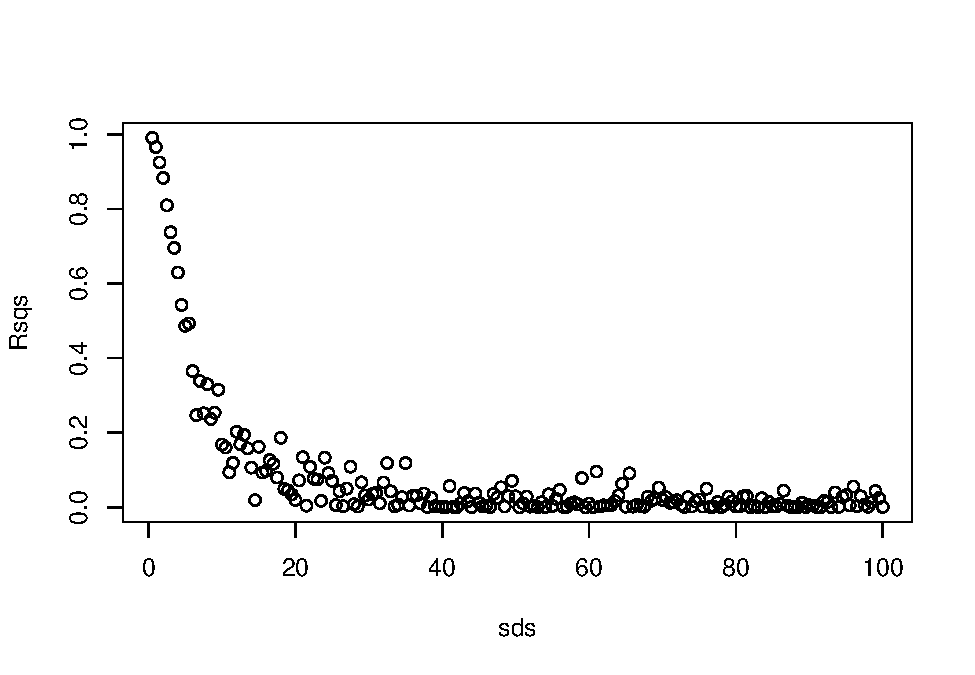
\includegraphics{ECOMODbook_files/figure-latex/unnamed-chunk-38-1.pdf}

How cool is that!! Actually, this means we can model the \(R^2\) as a function of the original variance! But we would not be able to model it using a linear model\ldots{}

You are not supposed to know about this yet, but I'll continue to show off. Let's use a GAM

\begin{Shaded}
\begin{Highlighting}[]
\KeywordTok{library}\NormalTok{(mgcv)}
\NormalTok{gam1=}\KeywordTok{gam}\NormalTok{(Rsqs}\OperatorTok{~}\KeywordTok{s}\NormalTok{(sds),}\DataTypeTok{link=}\NormalTok{log)}
\CommentTok{#make predictions to plot the estimated GAM model}
\NormalTok{predRsqs=}\KeywordTok{predict.gam}\NormalTok{(gam1,}\DataTypeTok{newdata =} \KeywordTok{list}\NormalTok{(}\DataTypeTok{sds=}\NormalTok{sds),}\DataTypeTok{type=}\StringTok{"response"}\NormalTok{)}
\KeywordTok{plot}\NormalTok{(sds,Rsqs)}
\KeywordTok{lines}\NormalTok{(sds,predRsqs,}\DataTypeTok{col=}\StringTok{"red"}\NormalTok{)}
\end{Highlighting}
\end{Shaded}

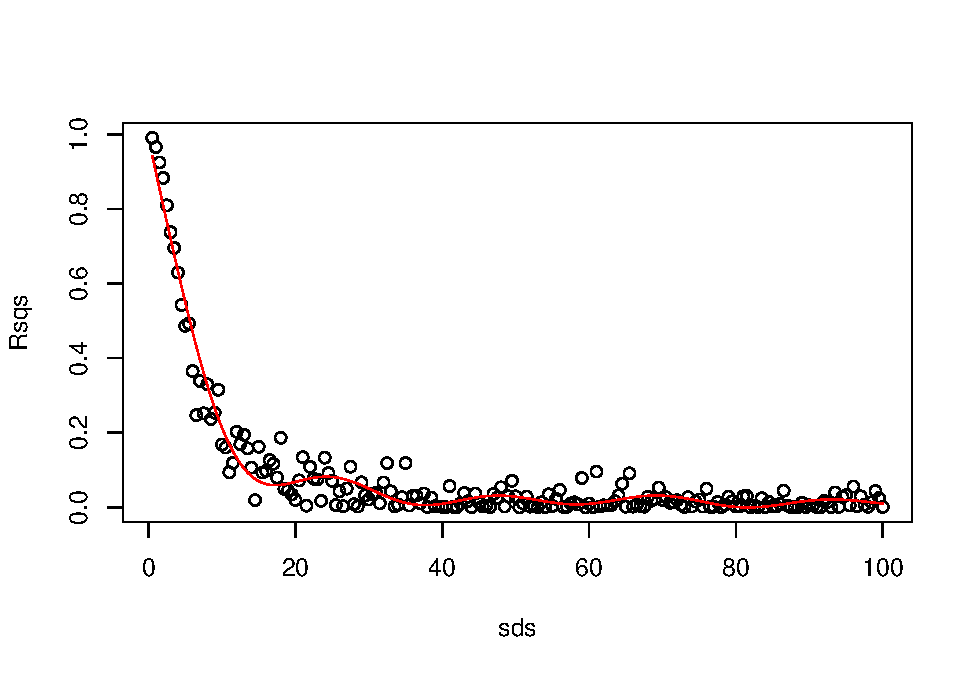
\includegraphics{ECOMODbook_files/figure-latex/unnamed-chunk-39-1.pdf}

Aha\ldots{} remember what we talked in class today? It seems like we have overfitted. Then, I constrain the GAM.

\begin{Shaded}
\begin{Highlighting}[]
\KeywordTok{library}\NormalTok{(mgcv)}
\NormalTok{gam1=}\KeywordTok{gam}\NormalTok{(Rsqs}\OperatorTok{~}\KeywordTok{s}\NormalTok{(sds,}\DataTypeTok{k=}\DecValTok{3}\NormalTok{),}\DataTypeTok{link=}\NormalTok{log)}
\CommentTok{#make predictions to plot the estimated GAM model}
\NormalTok{predRsqs=}\KeywordTok{predict.gam}\NormalTok{(gam1,}\DataTypeTok{newdata =} \KeywordTok{list}\NormalTok{(}\DataTypeTok{sds=}\NormalTok{sds),}\DataTypeTok{type=}\StringTok{"response"}\NormalTok{)}
\KeywordTok{plot}\NormalTok{(sds,Rsqs)}
\KeywordTok{lines}\NormalTok{(sds,predRsqs,}\DataTypeTok{col=}\StringTok{"red"}\NormalTok{)}
\end{Highlighting}
\end{Shaded}

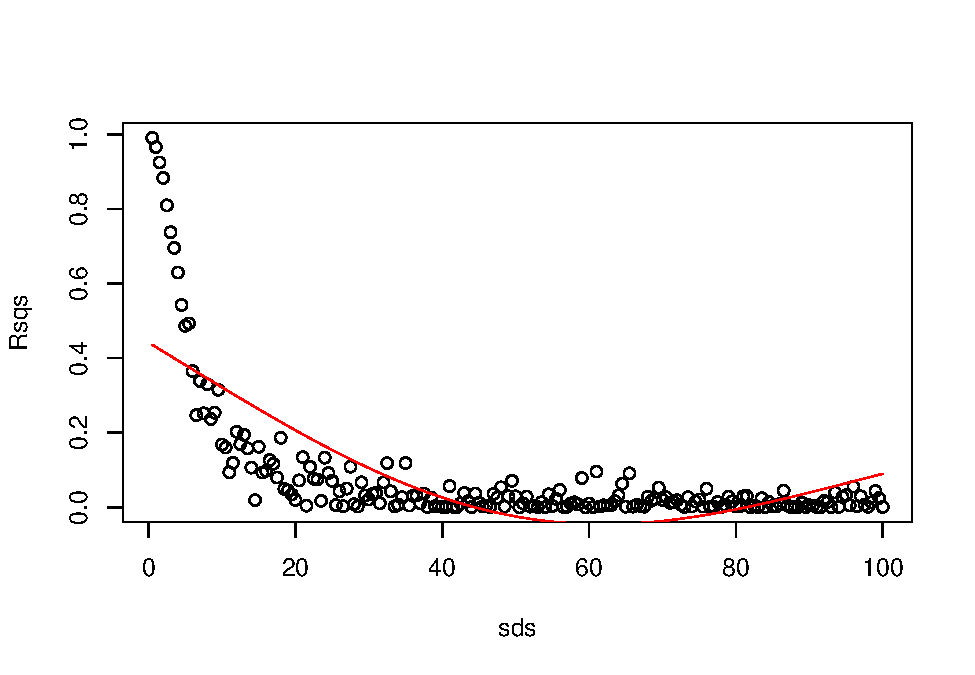
\includegraphics{ECOMODbook_files/figure-latex/unnamed-chunk-40-1.pdf}

That was too much\ldots{}

\begin{Shaded}
\begin{Highlighting}[]
\KeywordTok{library}\NormalTok{(mgcv)}
\NormalTok{gam1=}\KeywordTok{gam}\NormalTok{(Rsqs}\OperatorTok{~}\KeywordTok{s}\NormalTok{(sds,}\DataTypeTok{k=}\DecValTok{6}\NormalTok{),}\DataTypeTok{link=}\NormalTok{log)}
\CommentTok{#make predictions to plot the estimated GAM model}
\NormalTok{predRsqs=}\KeywordTok{predict.gam}\NormalTok{(gam1,}\DataTypeTok{newdata =} \KeywordTok{list}\NormalTok{(}\DataTypeTok{sds=}\NormalTok{sds),}\DataTypeTok{type=}\StringTok{"response"}\NormalTok{)}
\KeywordTok{plot}\NormalTok{(sds,Rsqs)}
\KeywordTok{lines}\NormalTok{(sds,predRsqs,}\DataTypeTok{col=}\StringTok{"red"}\NormalTok{)}
\end{Highlighting}
\end{Shaded}

\includegraphics{ECOMODbook_files/figure-latex/unnamed-chunk-41-1.pdf}

That is already overfitting\ldots{} conclusion, the GAM is not the right tool here :)

What is\ldots? Well, stay tuned and one day you'll learn!

\hypertarget{aula7}{%
\chapter{Class 7 14 10 2020}\label{aula7}}

In this class we continue exploring regression models, but we are going to increase their complexity. No longer just \texttt{a+bx}, but we add more explanatory variables. In particular, we will also add a factor covariate. And then we look under the hood to what that means.

\hypertarget{task-1}{%
\section{Task 1}\label{task-1}}

The first task the students were faced was to use some code to explore, by simulation, the impact of having variables in the model that are not relevant to explain the response. In particular, we wanted to identify when there would be no errors, or when there would be type I (a variable not relevant to explain the response is found relevant) and type II (a relevant variable to explain the response is not considered relevant) errors. For the sake of this example we consider a significance level of 5\%, but remember there is nothing sacred about it.

The guidelines provided were: ``Using the code below, and while changing the \texttt{seed} (\texttt{******} to begin with, so the code does not run as is!), explore how changing the parameters and the error leads to different amounts of type I and type II errors.''

\begin{Shaded}
\begin{Highlighting}[]
\CommentTok{# xs1 and xs2 wrong - type II error, xs3 and xs4 ok}
\NormalTok{seed<-}\ErrorTok{******}
\KeywordTok{set.seed}\NormalTok{(seed)}
\CommentTok{#define parameters}
\NormalTok{n<-}\DecValTok{50}\NormalTok{;b0<-}\DecValTok{5}\NormalTok{;b1<-}\DecValTok{3}\NormalTok{;b2<-}\OperatorTok{-}\DecValTok{2}\NormalTok{;error <-}\StringTok{ }\DecValTok{4}
\CommentTok{#simulate potential explanatory variables}
\NormalTok{xs1=}\KeywordTok{runif}\NormalTok{(n,}\DecValTok{10}\NormalTok{,}\DecValTok{20}\NormalTok{)}
\NormalTok{xs2=}\KeywordTok{runif}\NormalTok{(n,}\DecValTok{10}\NormalTok{,}\DecValTok{20}\NormalTok{)}
\NormalTok{xs3=}\KeywordTok{runif}\NormalTok{(n,}\DecValTok{10}\NormalTok{,}\DecValTok{20}\NormalTok{)}
\NormalTok{xs4=}\KeywordTok{runif}\NormalTok{(n,}\DecValTok{10}\NormalTok{,}\DecValTok{20}\NormalTok{)}
\CommentTok{#simulate response}
\NormalTok{ys=b0}\OperatorTok{+}\NormalTok{b1}\OperatorTok{*}\NormalTok{xs1}\OperatorTok{-}\NormalTok{b2}\OperatorTok{*}\NormalTok{xs2}\OperatorTok{+}\KeywordTok{rnorm}\NormalTok{(n,}\DataTypeTok{sd=}\NormalTok{error)}
\CommentTok{#plot data}
\KeywordTok{plot}\NormalTok{(xs1,ys)}
\CommentTok{#a model missing a variable, xs2}
\CommentTok{#summary(lm(ys~xs1))}
\CommentTok{#the true model}
\CommentTok{#summary(lm(ys~xs1+xs2))}
\CommentTok{#a model including irrelevant variables}
\KeywordTok{summary}\NormalTok{(}\KeywordTok{lm}\NormalTok{(ys}\OperatorTok{~}\NormalTok{xs1}\OperatorTok{+}\NormalTok{xs2}\OperatorTok{+}\NormalTok{xs3}\OperatorTok{+}\NormalTok{xs4))}
\end{Highlighting}
\end{Shaded}

The first thing to notice is that the model we simulate from only includes \texttt{xs1} and \texttt{xs2}. So, \texttt{xs3} and \texttt{xs4} do not have any impact on the response \texttt{y}

So we try different values for the seed and check what happens, Try \texttt{seed\textless{}-1}

\begin{Shaded}
\begin{Highlighting}[]
\NormalTok{seed<-}\DecValTok{1}
\KeywordTok{set.seed}\NormalTok{(seed)}
\CommentTok{#define parameters}
\NormalTok{n<-}\DecValTok{50}\NormalTok{;b0<-}\DecValTok{5}\NormalTok{;b1<-}\DecValTok{3}\NormalTok{;b2<-}\OperatorTok{-}\DecValTok{2}\NormalTok{;error <-}\StringTok{ }\DecValTok{4}
\CommentTok{#simulate potential explanatory variables}
\NormalTok{xs1=}\KeywordTok{runif}\NormalTok{(n,}\DecValTok{10}\NormalTok{,}\DecValTok{20}\NormalTok{)}
\NormalTok{xs2=}\KeywordTok{runif}\NormalTok{(n,}\DecValTok{10}\NormalTok{,}\DecValTok{20}\NormalTok{)}
\NormalTok{xs3=}\KeywordTok{runif}\NormalTok{(n,}\DecValTok{10}\NormalTok{,}\DecValTok{20}\NormalTok{)}
\NormalTok{xs4=}\KeywordTok{runif}\NormalTok{(n,}\DecValTok{10}\NormalTok{,}\DecValTok{20}\NormalTok{)}
\CommentTok{#simulate response}
\NormalTok{ys=b0}\OperatorTok{+}\NormalTok{b1}\OperatorTok{*}\NormalTok{xs1}\OperatorTok{-}\NormalTok{b2}\OperatorTok{*}\NormalTok{xs2}\OperatorTok{+}\KeywordTok{rnorm}\NormalTok{(n,}\DataTypeTok{sd=}\NormalTok{error)}
\CommentTok{#plot data}
\KeywordTok{plot}\NormalTok{(xs1,ys)}
\CommentTok{#look at model summary}
\KeywordTok{summary}\NormalTok{(}\KeywordTok{lm}\NormalTok{(ys}\OperatorTok{~}\NormalTok{xs1}\OperatorTok{+}\NormalTok{xs2}\OperatorTok{+}\NormalTok{xs3}\OperatorTok{+}\NormalTok{xs4))}
\end{Highlighting}
\end{Shaded}

All good, no errors. That is, \texttt{xs1} and \texttt{xs2} are considered statistically significant at th 5\% level and \texttt{xs3} and \texttt{xs4} are not found relevant to explain the response. Now, we keep changing \texttt{seed}

\begin{Shaded}
\begin{Highlighting}[]
\NormalTok{seed<-}\DecValTok{4}
\KeywordTok{set.seed}\NormalTok{(seed)}
\CommentTok{#define parameters}
\NormalTok{n<-}\DecValTok{50}\NormalTok{;b0<-}\DecValTok{5}\NormalTok{;b1<-}\DecValTok{3}\NormalTok{;b2<-}\OperatorTok{-}\DecValTok{2}\NormalTok{;error <-}\StringTok{ }\DecValTok{4}
\CommentTok{#simulate potential explanatory variables}
\NormalTok{xs1=}\KeywordTok{runif}\NormalTok{(n,}\DecValTok{10}\NormalTok{,}\DecValTok{20}\NormalTok{)}
\NormalTok{xs2=}\KeywordTok{runif}\NormalTok{(n,}\DecValTok{10}\NormalTok{,}\DecValTok{20}\NormalTok{)}
\NormalTok{xs3=}\KeywordTok{runif}\NormalTok{(n,}\DecValTok{10}\NormalTok{,}\DecValTok{20}\NormalTok{)}
\NormalTok{xs4=}\KeywordTok{runif}\NormalTok{(n,}\DecValTok{10}\NormalTok{,}\DecValTok{20}\NormalTok{)}
\CommentTok{#simulate response}
\NormalTok{ys=b0}\OperatorTok{+}\NormalTok{b1}\OperatorTok{*}\NormalTok{xs1}\OperatorTok{-}\NormalTok{b2}\OperatorTok{*}\NormalTok{xs2}\OperatorTok{+}\KeywordTok{rnorm}\NormalTok{(n,}\DataTypeTok{sd=}\NormalTok{error)}
\CommentTok{#plot data}
\KeywordTok{plot}\NormalTok{(xs1,ys)}
\CommentTok{#look at model summary}
\KeywordTok{summary}\NormalTok{(}\KeywordTok{lm}\NormalTok{(ys}\OperatorTok{~}\NormalTok{xs1}\OperatorTok{+}\NormalTok{xs2}\OperatorTok{+}\NormalTok{xs3}\OperatorTok{+}\NormalTok{xs4))}
\end{Highlighting}
\end{Shaded}

We find our first type I error, \texttt{xs4} is found statistically significant, but we know it has no effect on the response. The same happens with \texttt{seed} being e.g.~9, 10. When we try \texttt{seed\ \textless{}-\ 11} we get another type I error, this time on \texttt{xs4}

\begin{Shaded}
\begin{Highlighting}[]
\NormalTok{seed<-}\DecValTok{11}
\KeywordTok{set.seed}\NormalTok{(seed)}
\CommentTok{#define parameters}
\NormalTok{n<-}\DecValTok{50}\NormalTok{;b0<-}\DecValTok{5}\NormalTok{;b1<-}\DecValTok{3}\NormalTok{;b2<-}\OperatorTok{-}\DecValTok{2}\NormalTok{;error <-}\StringTok{ }\DecValTok{4}
\CommentTok{#simulate potential explanatory variables}
\NormalTok{xs1=}\KeywordTok{runif}\NormalTok{(n,}\DecValTok{10}\NormalTok{,}\DecValTok{20}\NormalTok{)}
\NormalTok{xs2=}\KeywordTok{runif}\NormalTok{(n,}\DecValTok{10}\NormalTok{,}\DecValTok{20}\NormalTok{)}
\NormalTok{xs3=}\KeywordTok{runif}\NormalTok{(n,}\DecValTok{10}\NormalTok{,}\DecValTok{20}\NormalTok{)}
\NormalTok{xs4=}\KeywordTok{runif}\NormalTok{(n,}\DecValTok{10}\NormalTok{,}\DecValTok{20}\NormalTok{)}
\CommentTok{#simulate response}
\NormalTok{ys=b0}\OperatorTok{+}\NormalTok{b1}\OperatorTok{*}\NormalTok{xs1}\OperatorTok{-}\NormalTok{b2}\OperatorTok{*}\NormalTok{xs2}\OperatorTok{+}\KeywordTok{rnorm}\NormalTok{(n,}\DataTypeTok{sd=}\NormalTok{error)}
\CommentTok{#plot data}
\KeywordTok{plot}\NormalTok{(xs1,ys)}
\end{Highlighting}
\end{Shaded}

\includegraphics{ECOMODbook_files/figure-latex/unnamed-chunk-45-1.pdf}

\begin{Shaded}
\begin{Highlighting}[]
\CommentTok{#look at model summary}
\KeywordTok{summary}\NormalTok{(}\KeywordTok{lm}\NormalTok{(ys}\OperatorTok{~}\NormalTok{xs1}\OperatorTok{+}\NormalTok{xs2}\OperatorTok{+}\NormalTok{xs3}\OperatorTok{+}\NormalTok{xs4))}
\end{Highlighting}
\end{Shaded}

\begin{verbatim}
## 
## Call:
## lm(formula = ys ~ xs1 + xs2 + xs3 + xs4)
## 
## Residuals:
##      Min       1Q   Median       3Q      Max 
## -10.3076  -2.7316   0.3072   2.2102   7.9088 
## 
## Coefficients:
##             Estimate Std. Error t value Pr(>|t|)    
## (Intercept) 16.44303    7.42710   2.214   0.0319 *  
## xs1          2.87327    0.21665  13.262  < 2e-16 ***
## xs2          1.93313    0.25274   7.649 1.12e-09 ***
## xs3         -0.47689    0.22325  -2.136   0.0381 *  
## xs4         -0.08922    0.20937  -0.426   0.6720    
## ---
## Signif. codes:  0 '***' 0.001 '**' 0.01 '*' 0.05 '.' 0.1 ' ' 1
## 
## Residual standard error: 4.074 on 45 degrees of freedom
## Multiple R-squared:  0.8484,	Adjusted R-squared:  0.8349 
## F-statistic: 62.94 on 4 and 45 DF,  p-value: < 2.2e-16
\end{verbatim}

However, even after several runs, we never make a type II error. That must mean this setting has a large power, i.e.~the ability to detect a true effect when one exists. Well, there are many ways to decrease power, like having a smaller sample size, increase the error or lower the true effect. Let's try to increase the error, instead of the 4 used above, let's pump it up10 fold to 40

\begin{Shaded}
\begin{Highlighting}[]
\NormalTok{seed<-}\DecValTok{100}
\KeywordTok{set.seed}\NormalTok{(seed)}
\CommentTok{#define parameters}
\NormalTok{n<-}\DecValTok{50}\NormalTok{;b0<-}\DecValTok{5}\NormalTok{;b1<-}\DecValTok{3}\NormalTok{;b2<-}\OperatorTok{-}\DecValTok{2}\NormalTok{;error <-}\StringTok{ }\DecValTok{40}
\CommentTok{#simulate potential explanatory variables}
\NormalTok{xs1=}\KeywordTok{runif}\NormalTok{(n,}\DecValTok{10}\NormalTok{,}\DecValTok{20}\NormalTok{)}
\NormalTok{xs2=}\KeywordTok{runif}\NormalTok{(n,}\DecValTok{10}\NormalTok{,}\DecValTok{20}\NormalTok{)}
\NormalTok{xs3=}\KeywordTok{runif}\NormalTok{(n,}\DecValTok{10}\NormalTok{,}\DecValTok{20}\NormalTok{)}
\NormalTok{xs4=}\KeywordTok{runif}\NormalTok{(n,}\DecValTok{10}\NormalTok{,}\DecValTok{20}\NormalTok{)}
\CommentTok{#simulate response}
\NormalTok{ys=b0}\OperatorTok{+}\NormalTok{b1}\OperatorTok{*}\NormalTok{xs1}\OperatorTok{-}\NormalTok{b2}\OperatorTok{*}\NormalTok{xs2}\OperatorTok{+}\KeywordTok{rnorm}\NormalTok{(n,}\DataTypeTok{sd=}\NormalTok{error)}
\CommentTok{#plot data}
\KeywordTok{plot}\NormalTok{(xs1,ys)}
\end{Highlighting}
\end{Shaded}

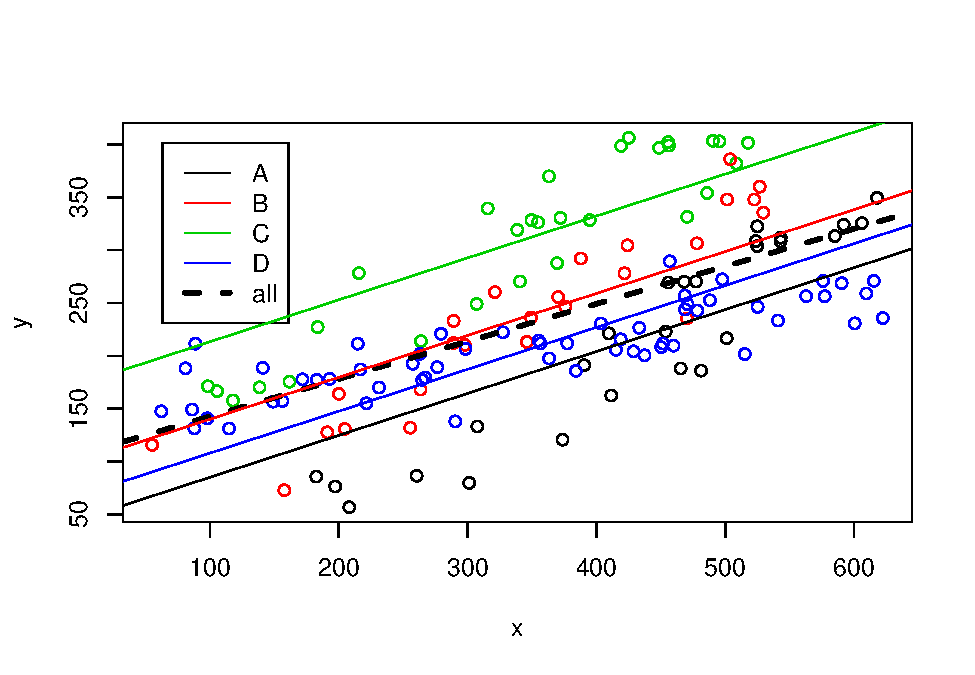
\includegraphics{ECOMODbook_files/figure-latex/unnamed-chunk-46-1.pdf}

\begin{Shaded}
\begin{Highlighting}[]
\CommentTok{#look at model summary}
\KeywordTok{summary}\NormalTok{(}\KeywordTok{lm}\NormalTok{(ys}\OperatorTok{~}\NormalTok{xs1}\OperatorTok{+}\NormalTok{xs2}\OperatorTok{+}\NormalTok{xs3}\OperatorTok{+}\NormalTok{xs4))}
\end{Highlighting}
\end{Shaded}

\begin{verbatim}
## 
## Call:
## lm(formula = ys ~ xs1 + xs2 + xs3 + xs4)
## 
## Residuals:
##    Min     1Q Median     3Q    Max 
## -73.25 -17.86  -6.76  21.25  68.42 
## 
## Coefficients:
##             Estimate Std. Error t value Pr(>|t|)
## (Intercept)  22.8661    41.3133   0.553    0.583
## xs1           1.6034     1.8564   0.864    0.392
## xs2           0.9163     1.8092   0.506    0.615
## xs3           1.9650     1.6038   1.225    0.227
## xs4          -0.8544     1.7449  -0.490    0.627
## 
## Residual standard error: 32.4 on 45 degrees of freedom
## Multiple R-squared:  0.06896,	Adjusted R-squared:  -0.0138 
## F-statistic: 0.8333 on 4 and 45 DF,  p-value: 0.5112
\end{verbatim}

That was an overkill, now there is so much noise must seeds we use do not allow us to find an effect, let's cut that in half to 20

\begin{Shaded}
\begin{Highlighting}[]
\NormalTok{seed<-}\DecValTok{100}
\KeywordTok{set.seed}\NormalTok{(seed)}
\CommentTok{#define parameters}
\NormalTok{n<-}\DecValTok{50}\NormalTok{;b0<-}\DecValTok{5}\NormalTok{;b1<-}\DecValTok{3}\NormalTok{;b2<-}\OperatorTok{-}\DecValTok{2}\NormalTok{;error <-}\StringTok{ }\DecValTok{20}
\CommentTok{#simulate potential explanatory variables}
\NormalTok{xs1=}\KeywordTok{runif}\NormalTok{(n,}\DecValTok{10}\NormalTok{,}\DecValTok{20}\NormalTok{)}
\NormalTok{xs2=}\KeywordTok{runif}\NormalTok{(n,}\DecValTok{10}\NormalTok{,}\DecValTok{20}\NormalTok{)}
\NormalTok{xs3=}\KeywordTok{runif}\NormalTok{(n,}\DecValTok{10}\NormalTok{,}\DecValTok{20}\NormalTok{)}
\NormalTok{xs4=}\KeywordTok{runif}\NormalTok{(n,}\DecValTok{10}\NormalTok{,}\DecValTok{20}\NormalTok{)}
\CommentTok{#simulate response}
\NormalTok{ys=b0}\OperatorTok{+}\NormalTok{b1}\OperatorTok{*}\NormalTok{xs1}\OperatorTok{-}\NormalTok{b2}\OperatorTok{*}\NormalTok{xs2}\OperatorTok{+}\KeywordTok{rnorm}\NormalTok{(n,}\DataTypeTok{sd=}\NormalTok{error)}
\CommentTok{#plot data}
\KeywordTok{plot}\NormalTok{(xs1,ys)}
\end{Highlighting}
\end{Shaded}

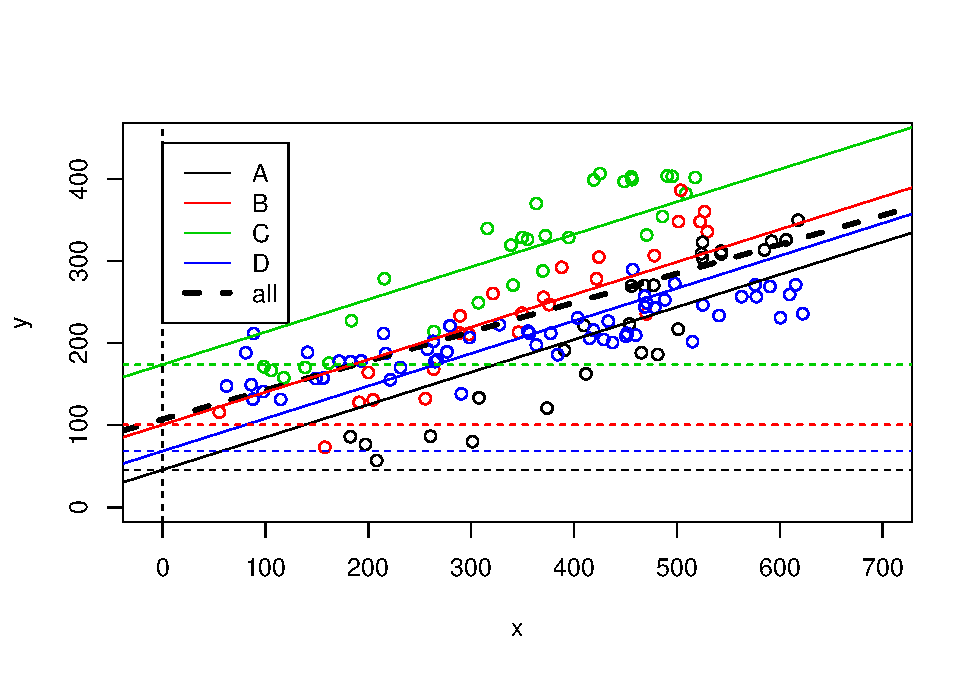
\includegraphics{ECOMODbook_files/figure-latex/unnamed-chunk-47-1.pdf}

\begin{Shaded}
\begin{Highlighting}[]
\CommentTok{#look at model summary}
\KeywordTok{summary}\NormalTok{(}\KeywordTok{lm}\NormalTok{(ys}\OperatorTok{~}\NormalTok{xs1}\OperatorTok{+}\NormalTok{xs2}\OperatorTok{+}\NormalTok{xs3}\OperatorTok{+}\NormalTok{xs4))}
\end{Highlighting}
\end{Shaded}

\begin{verbatim}
## 
## Call:
## lm(formula = ys ~ xs1 + xs2 + xs3 + xs4)
## 
## Residuals:
##     Min      1Q  Median      3Q     Max 
## -36.624  -8.927  -3.380  10.623  34.211 
## 
## Coefficients:
##             Estimate Std. Error t value Pr(>|t|)  
## (Intercept)  13.9330    20.6566   0.675    0.503  
## xs1           2.3017     0.9282   2.480    0.017 *
## xs2           1.4582     0.9046   1.612    0.114  
## xs3           0.9825     0.8019   1.225    0.227  
## xs4          -0.4272     0.8724  -0.490    0.627  
## ---
## Signif. codes:  0 '***' 0.001 '**' 0.01 '*' 0.05 '.' 0.1 ' ' 1
## 
## Residual standard error: 16.2 on 45 degrees of freedom
## Multiple R-squared:  0.2262,	Adjusted R-squared:  0.1574 
## F-statistic: 3.288 on 4 and 45 DF,  p-value: 0.01901
\end{verbatim}

back to all correct. Now, let's change seed again

\begin{Shaded}
\begin{Highlighting}[]
\NormalTok{seed<-}\DecValTok{103}
\KeywordTok{set.seed}\NormalTok{(seed)}
\CommentTok{#define parameters}
\NormalTok{n<-}\DecValTok{50}\NormalTok{;b0<-}\DecValTok{5}\NormalTok{;b1<-}\DecValTok{3}\NormalTok{;b2<-}\OperatorTok{-}\DecValTok{2}\NormalTok{;error <-}\StringTok{ }\DecValTok{20}
\CommentTok{#simulate potential explanatory variables}
\NormalTok{xs1=}\KeywordTok{runif}\NormalTok{(n,}\DecValTok{10}\NormalTok{,}\DecValTok{20}\NormalTok{)}
\NormalTok{xs2=}\KeywordTok{runif}\NormalTok{(n,}\DecValTok{10}\NormalTok{,}\DecValTok{20}\NormalTok{)}
\NormalTok{xs3=}\KeywordTok{runif}\NormalTok{(n,}\DecValTok{10}\NormalTok{,}\DecValTok{20}\NormalTok{)}
\NormalTok{xs4=}\KeywordTok{runif}\NormalTok{(n,}\DecValTok{10}\NormalTok{,}\DecValTok{20}\NormalTok{)}
\CommentTok{#simulate response}
\NormalTok{ys=b0}\OperatorTok{+}\NormalTok{b1}\OperatorTok{*}\NormalTok{xs1}\OperatorTok{-}\NormalTok{b2}\OperatorTok{*}\NormalTok{xs2}\OperatorTok{+}\KeywordTok{rnorm}\NormalTok{(n,}\DataTypeTok{sd=}\NormalTok{error)}
\CommentTok{#plot data}
\KeywordTok{plot}\NormalTok{(xs1,ys)}
\end{Highlighting}
\end{Shaded}

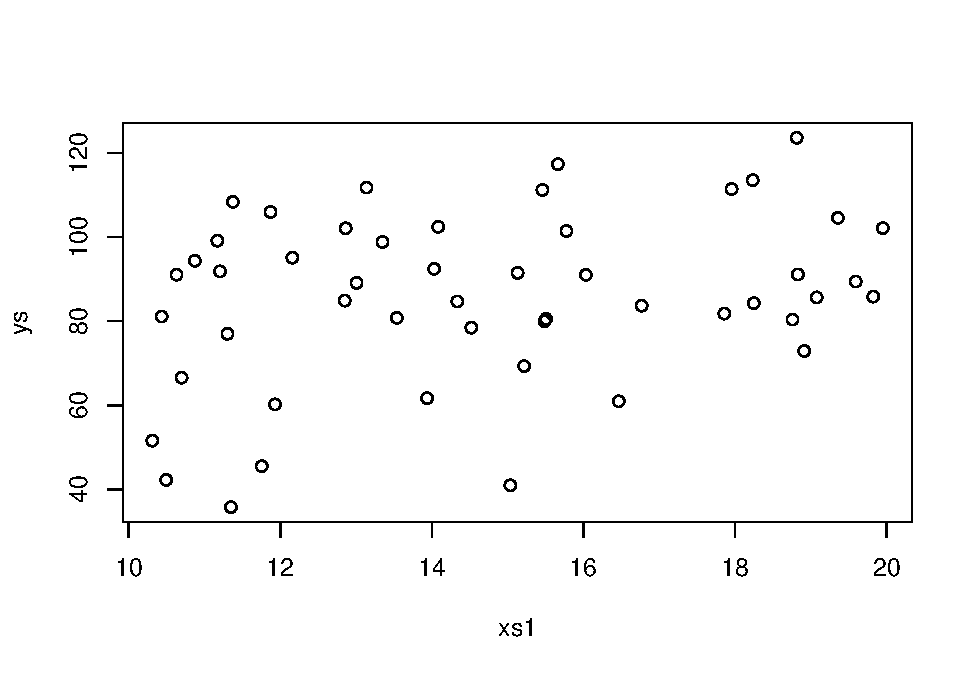
\includegraphics{ECOMODbook_files/figure-latex/unnamed-chunk-48-1.pdf}

\begin{Shaded}
\begin{Highlighting}[]
\CommentTok{#look at model summary}
\KeywordTok{summary}\NormalTok{(}\KeywordTok{lm}\NormalTok{(ys}\OperatorTok{~}\NormalTok{xs1}\OperatorTok{+}\NormalTok{xs2}\OperatorTok{+}\NormalTok{xs3}\OperatorTok{+}\NormalTok{xs4))}
\end{Highlighting}
\end{Shaded}

\begin{verbatim}
## 
## Call:
## lm(formula = ys ~ xs1 + xs2 + xs3 + xs4)
## 
## Residuals:
##     Min      1Q  Median      3Q     Max 
## -36.079 -10.686  -0.148  16.413  33.845 
## 
## Coefficients:
##             Estimate Std. Error t value Pr(>|t|)  
## (Intercept)  9.70575   33.83339   0.287   0.7755  
## xs1          2.32559    0.93980   2.475   0.0172 *
## xs2          1.97688    1.20464   1.641   0.1078  
## xs3          0.69013    1.02110   0.676   0.5026  
## xs4          0.08031    0.97427   0.082   0.9347  
## ---
## Signif. codes:  0 '***' 0.001 '**' 0.01 '*' 0.05 '.' 0.1 ' ' 1
## 
## Residual standard error: 19.6 on 45 degrees of freedom
## Multiple R-squared:  0.1524,	Adjusted R-squared:  0.07706 
## F-statistic: 2.023 on 4 and 45 DF,  p-value: 0.1073
\end{verbatim}

Bang on, a type II error, as \texttt{xs2} is no longer considered statistically significant. I am sure you can now play with the relevant model parameters, \texttt{b1}, \texttt{b2}, to incleare and decreese the actual effect, and with sample size \texttt{n} or as above with the \texttt{error} and explore the consequences of changing the balance in effect size, error and sample size on the ability of incurring in errors when doing regression. But remmeber the key, the reason we are able to see if an error is made or not is because we simulated reality. In this case, as it is never the case in an ecological dataset, we know the true model, which was

\[y=\beta_0+\beta_1 xs_1+\beta_2 xs2\]

That is the luxury of simulation, allowing you to test scenarios where ``reality'' is known, hence evaluating methods performance.

\begin{Shaded}
\begin{Highlighting}[]
\NormalTok{folder<-}\StringTok{"extfiles/"}
\CommentTok{#folder<-"../Aula7 14 10 2020/"}
\NormalTok{d4l <-}\StringTok{ }\KeywordTok{read.csv}\NormalTok{(}\DataTypeTok{file=}\KeywordTok{paste0}\NormalTok{(folder,}\StringTok{"data4lines.csv"}\NormalTok{))}
\NormalTok{n <-}\StringTok{ }\KeywordTok{nrow}\NormalTok{(d4l)}
\end{Highlighting}
\end{Shaded}

\hypertarget{task-2}{%
\section{Task 2}\label{task-2}}

The second task the students were faced was to create some regression data and the explore fitting models to it.

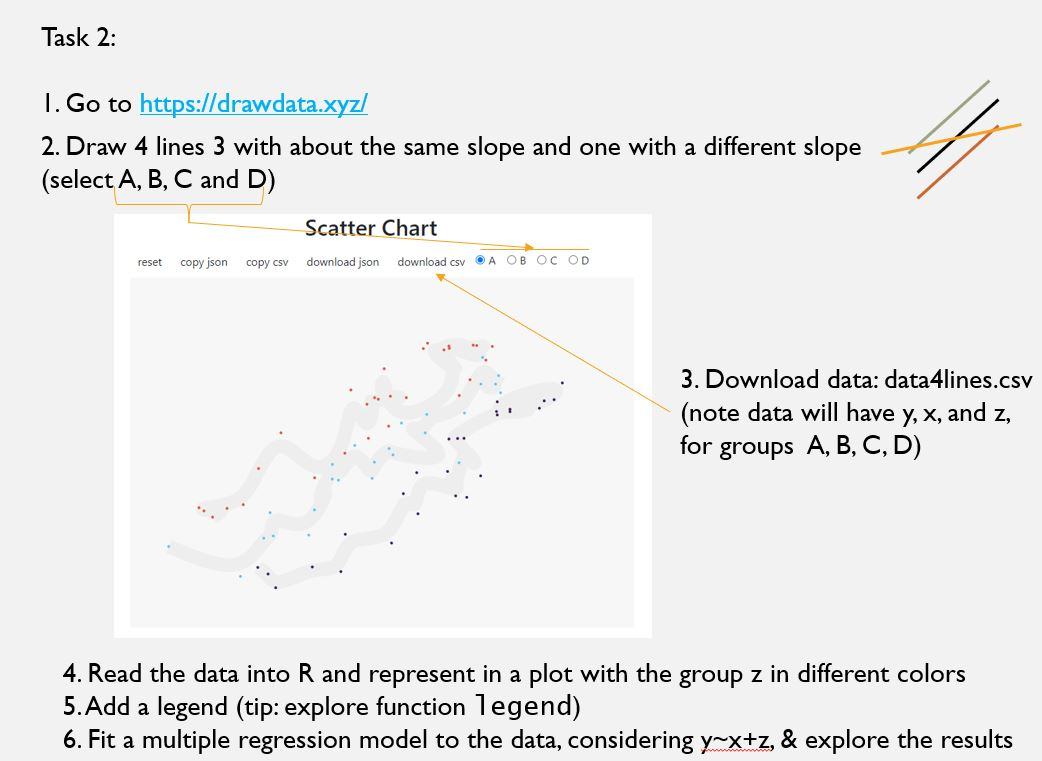
\includegraphics{extfiles/Aula7Task7.JPG}

The data was simulated via this website: \url{https://drawdata.xyz/} and was named \texttt{data4lines.csv}. Each student had its own dataset, here I work with my example.

We begin by reading the data in and plot it

\begin{Shaded}
\begin{Highlighting}[]
\CommentTok{#read the data}
\CommentTok{#folder<-"../Aula7 14 10 2020/"}
\NormalTok{folder<-}\StringTok{"extfiles/"}
\NormalTok{data4lines <-}\StringTok{ }\KeywordTok{read.csv}\NormalTok{(}\DataTypeTok{file=}\KeywordTok{paste0}\NormalTok{(folder,}\StringTok{"data4lines.csv"}\NormalTok{))}
\CommentTok{#plot all the data}
\KeywordTok{plot}\NormalTok{(y}\OperatorTok{~}\NormalTok{x,}\DataTypeTok{data=}\NormalTok{data4lines)}
\end{Highlighting}
\end{Shaded}

\includegraphics{ECOMODbook_files/figure-latex/unnamed-chunk-50-1.pdf}

Now, to turn this a bit more interesting, we come up with a narrative.

These correspond to observations from weights and lenghts of a sample of animals, fish from the species \emph{Fishus inventadicus}. We could fit a regression line to this data and see if we can predict weight from length

\begin{Shaded}
\begin{Highlighting}[]
\CommentTok{#plot all the data}
\KeywordTok{plot}\NormalTok{(y}\OperatorTok{~}\NormalTok{x,}\DataTypeTok{data=}\NormalTok{data4lines)}
\CommentTok{#fit model to pooled data}
\NormalTok{lmlinesG<-}\KeywordTok{lm}\NormalTok{(y}\OperatorTok{~}\NormalTok{x,}\DataTypeTok{data=}\NormalTok{data4lines)}
\KeywordTok{abline}\NormalTok{(lmlinesG,}\DataTypeTok{lwd=}\DecValTok{3}\NormalTok{,}\DataTypeTok{lty=}\DecValTok{2}\NormalTok{)}
\end{Highlighting}
\end{Shaded}

\includegraphics{ECOMODbook_files/figure-latex/unnamed-chunk-51-1.pdf}

\begin{Shaded}
\begin{Highlighting}[]
\KeywordTok{summary}\NormalTok{(lmlinesG)}
\end{Highlighting}
\end{Shaded}

\begin{verbatim}
## 
## Call:
## lm(formula = y ~ x, data = data4lines)
## 
## Residuals:
##      Min       1Q   Median       3Q      Max 
## -134.304  -44.188   -1.995   29.432  148.202 
## 
## Coefficients:
##              Estimate Std. Error t value Pr(>|t|)    
## (Intercept) 107.17590   14.03069   7.639 3.51e-12 ***
## x             0.35513    0.03553   9.995  < 2e-16 ***
## ---
## Signif. codes:  0 '***' 0.001 '**' 0.01 '*' 0.05 '.' 0.1 ' ' 1
## 
## Residual standard error: 61.78 on 136 degrees of freedom
## Multiple R-squared:  0.4235,	Adjusted R-squared:  0.4193 
## F-statistic: 99.91 on 1 and 136 DF,  p-value: < 2.2e-16
\end{verbatim}

and it looks like we can indeed predict the weight of the species from its length. The length is higly statistically significant. Not surprisingly, the longer the fish the heavier it is.

Now, the plot thickens. These animals actually came from 4 different museums, and are assumed to be the same species. However, a scientis decides to look at wether there are differences in the data from the 4 museums. So he colours the data by museum

\begin{Shaded}
\begin{Highlighting}[]
\CommentTok{#plot all the data}
\KeywordTok{plot}\NormalTok{(y}\OperatorTok{~}\NormalTok{x,}\DataTypeTok{col=}\KeywordTok{as.numeric}\NormalTok{(}\KeywordTok{as.factor}\NormalTok{(z)),}\DataTypeTok{data=}\NormalTok{data4lines,}\DataTypeTok{pch=}\DecValTok{1}\NormalTok{)}
\KeywordTok{legend}\NormalTok{(}\StringTok{"topleft"}\NormalTok{,}\DataTypeTok{inset=}\FloatTok{0.05}\NormalTok{,}\DataTypeTok{legend=}\NormalTok{letters[}\DecValTok{1}\OperatorTok{:}\DecValTok{4}\NormalTok{],}\DataTypeTok{col=}\DecValTok{1}\OperatorTok{:}\DecValTok{4}\NormalTok{,}\DataTypeTok{pch=}\DecValTok{1}\NormalTok{)}
\end{Highlighting}
\end{Shaded}

\includegraphics{ECOMODbook_files/figure-latex/unnamed-chunk-52-1.pdf}

We see a patter in the data, the data from the different museums tend to cluster. He decides to investigate. Note folks providing names to museum in this country are a bit borring, and the museums are called ``a'', ``b'', ``c'' and ``d''.

Our smart researcher says: ``well, it seems like the relationship might be different in each museum''. Then, maybe I should fit a model that includes museum as a covariate \texttt{weight\textasciitilde{}length+museum}.

\[y=\beta_0+\beta_1 \times length +\beta_2 \times museum\]

And so he does and plots it

\begin{Shaded}
\begin{Highlighting}[]
\CommentTok{#fit model per group}
\NormalTok{lmlines<-}\KeywordTok{lm}\NormalTok{(y}\OperatorTok{~}\NormalTok{x}\OperatorTok{+}\NormalTok{z,}\DataTypeTok{data=}\NormalTok{data4lines)}
\KeywordTok{summary}\NormalTok{(lmlines)}
\end{Highlighting}
\end{Shaded}

\begin{verbatim}
## 
## Call:
## lm(formula = y ~ x + z, data = data4lines)
## 
## Residuals:
##    Min     1Q Median     3Q    Max 
## -90.01 -35.01   2.54  35.51 108.10 
## 
## Coefficients:
##              Estimate Std. Error t value Pr(>|t|)    
## (Intercept)  45.51813   13.83069   3.291  0.00128 ** 
## x             0.39657    0.02516  15.763  < 2e-16 ***
## zb           54.92376   12.11597   4.533 1.28e-05 ***
## zc          128.20339   11.72572  10.934  < 2e-16 ***
## zd           22.82412   10.26509   2.223  0.02787 *  
## ---
## Signif. codes:  0 '***' 0.001 '**' 0.01 '*' 0.05 '.' 0.1 ' ' 1
## 
## Residual standard error: 42.5 on 133 degrees of freedom
## Multiple R-squared:  0.7332,	Adjusted R-squared:  0.7252 
## F-statistic: 91.38 on 4 and 133 DF,  p-value: < 2.2e-16
\end{verbatim}

The output shows that the length is relevant, but the museum is relevant too. The relationship might be different per museum! In the output we see the \texttt{x}, the length, but not the \texttt{z}, it has been transformed into \texttt{zb}, \texttt{zc} and \texttt{zd}. Why is that? That is a mistery that we shall unfold now!

While the model we are fitting might be represented by \texttt{weight\textasciitilde{}length+museum}, th edesign matrix being fitted replaces the \texttt{museum} (a factor with 4 levels) with 3 dummy variables (a factor with k levels required k-1 dummy variables). So the real model being fitted is really

\[y=\beta_0+\beta_1 \times length + \beta_{2b} \times zb + \beta_{2c} \times zc + \beta_{2d} \times zd\]

Wait, but where is the level \texttt{a}? It is in the intercept, and if I had an euro for each time that confused a student, I would not be here but in a beach in the Bahamas having a piña colada :)

But let's unfold the mistery, shall we? By default, R takes 1 level of (each/a) factor and uses it as the intercept. Here it used \texttt{a} (the choice is in this case by alphabetical ored, but one can change that, which might be useful if e.g.~you want to have as the intercept a control level, say; look e.g.~into function \texttt{factor} help to see how you can change the baseline \texttt{level} of a factor).

Hence, the intercept for museum \texttt{a} is 45.5181335. What about the intercep of the othe rmuseums? They are always reported with \texttt{a} as the reference. Look at the equation above, what happens when say zc is 1 and zd and zb are 0, it becomes

\[y=\beta_0+\beta_1 \times length + \beta_{2c} \times zc \]
\[y=(\beta_0+\beta_{2c})+\beta_1 \times length = intercep + slope \times length\]

and so, from the above output, that equates to \texttt{y=lmlines\$coefficients{[}1{]}+lmlines\$coefficients{[}4{]},lmlines\$coefficients{[}2{]}} or 173.7215247+0.3965715 \(\times\) \texttt{length}.

So now we can add all these estimated regression lines to the plot

\begin{Shaded}
\begin{Highlighting}[]
\CommentTok{#plot all}
\KeywordTok{plot}\NormalTok{(y}\OperatorTok{~}\NormalTok{x,}\DataTypeTok{col=}\NormalTok{z,}\DataTypeTok{data=}\NormalTok{data4lines)}
\KeywordTok{legend}\NormalTok{(}\StringTok{"topleft"}\NormalTok{,}\DataTypeTok{inset=}\FloatTok{0.05}\NormalTok{,}\DataTypeTok{legend=}\KeywordTok{c}\NormalTok{(LETTERS[}\DecValTok{1}\OperatorTok{:}\DecValTok{4}\NormalTok{],}\StringTok{"all"}\NormalTok{),}\DataTypeTok{col=}\KeywordTok{c}\NormalTok{(}\DecValTok{1}\OperatorTok{:}\DecValTok{4}\NormalTok{,}\DecValTok{1}\NormalTok{),}\DataTypeTok{lty=}\KeywordTok{c}\NormalTok{(}\KeywordTok{rep}\NormalTok{(}\DecValTok{1}\NormalTok{,}\DecValTok{4}\NormalTok{),}\DecValTok{2}\NormalTok{),}\DataTypeTok{lwd=}\KeywordTok{c}\NormalTok{(}\KeywordTok{rep}\NormalTok{(}\DecValTok{1}\NormalTok{,}\DecValTok{4}\NormalTok{),}\DecValTok{3}\NormalTok{))}
\CommentTok{#these are the wrong lines... why?}
\KeywordTok{abline}\NormalTok{(lmlinesG,}\DataTypeTok{lwd=}\DecValTok{3}\NormalTok{,}\DataTypeTok{lty=}\DecValTok{2}\NormalTok{)}
\KeywordTok{abline}\NormalTok{(lmlines}\OperatorTok{$}\NormalTok{coefficients[}\DecValTok{1}\NormalTok{],lmlines}\OperatorTok{$}\NormalTok{coefficients[}\DecValTok{2}\NormalTok{],}\DataTypeTok{col=}\DecValTok{1}\NormalTok{)}
\KeywordTok{abline}\NormalTok{(lmlines}\OperatorTok{$}\NormalTok{coefficients[}\DecValTok{1}\NormalTok{]}\OperatorTok{+}\NormalTok{lmlines}\OperatorTok{$}\NormalTok{coefficients[}\DecValTok{3}\NormalTok{],lmlines}\OperatorTok{$}\NormalTok{coefficients[}\DecValTok{2}\NormalTok{],}\DataTypeTok{col=}\DecValTok{2}\NormalTok{)}
\KeywordTok{abline}\NormalTok{(lmlines}\OperatorTok{$}\NormalTok{coefficients[}\DecValTok{1}\NormalTok{]}\OperatorTok{+}\NormalTok{lmlines}\OperatorTok{$}\NormalTok{coefficients[}\DecValTok{4}\NormalTok{],lmlines}\OperatorTok{$}\NormalTok{coefficients[}\DecValTok{2}\NormalTok{],}\DataTypeTok{col=}\DecValTok{3}\NormalTok{)}
\KeywordTok{abline}\NormalTok{(lmlines}\OperatorTok{$}\NormalTok{coefficients[}\DecValTok{1}\NormalTok{]}\OperatorTok{+}\NormalTok{lmlines}\OperatorTok{$}\NormalTok{coefficients[}\DecValTok{5}\NormalTok{],lmlines}\OperatorTok{$}\NormalTok{coefficients[}\DecValTok{2}\NormalTok{],}\DataTypeTok{col=}\DecValTok{4}\NormalTok{)}
\end{Highlighting}
\end{Shaded}

\includegraphics{ECOMODbook_files/figure-latex/unnamed-chunk-54-1.pdf}

note that, not surprisingly, all these lines have the same slope. Or in other words, the model we considered assumes that the slope of the model is the same across museums (which, remember, we know if not true!). We can easily check that the intercepts (i.e.~where the lines cross when length=x=0) of all lines are indeed easy to get from the model's output

\begin{Shaded}
\begin{Highlighting}[]
\CommentTok{#plot all}
\KeywordTok{plot}\NormalTok{(y}\OperatorTok{~}\NormalTok{x,}\DataTypeTok{xlim=}\KeywordTok{c}\NormalTok{(}\OperatorTok{-}\DecValTok{10}\NormalTok{,}\DecValTok{700}\NormalTok{),}\DataTypeTok{ylim=}\KeywordTok{c}\NormalTok{(}\DecValTok{0}\NormalTok{,}\DecValTok{450}\NormalTok{),}\DataTypeTok{col=}\NormalTok{z,}\DataTypeTok{data=}\NormalTok{data4lines)}
\KeywordTok{legend}\NormalTok{(}\StringTok{"topleft"}\NormalTok{,}\DataTypeTok{inset=}\FloatTok{0.05}\NormalTok{,}\DataTypeTok{legend=}\KeywordTok{c}\NormalTok{(LETTERS[}\DecValTok{1}\OperatorTok{:}\DecValTok{4}\NormalTok{],}\StringTok{"all"}\NormalTok{),}\DataTypeTok{col=}\KeywordTok{c}\NormalTok{(}\DecValTok{1}\OperatorTok{:}\DecValTok{4}\NormalTok{,}\DecValTok{1}\NormalTok{),}\DataTypeTok{lty=}\KeywordTok{c}\NormalTok{(}\KeywordTok{rep}\NormalTok{(}\DecValTok{1}\NormalTok{,}\DecValTok{4}\NormalTok{),}\DecValTok{2}\NormalTok{),}\DataTypeTok{lwd=}\KeywordTok{c}\NormalTok{(}\KeywordTok{rep}\NormalTok{(}\DecValTok{1}\NormalTok{,}\DecValTok{4}\NormalTok{),}\DecValTok{3}\NormalTok{))}
\CommentTok{#these are the wrong lines... why?}
\KeywordTok{abline}\NormalTok{(lmlinesG,}\DataTypeTok{lwd=}\DecValTok{3}\NormalTok{,}\DataTypeTok{lty=}\DecValTok{2}\NormalTok{)}
\KeywordTok{abline}\NormalTok{(lmlines}\OperatorTok{$}\NormalTok{coefficients[}\DecValTok{1}\NormalTok{],lmlines}\OperatorTok{$}\NormalTok{coefficients[}\DecValTok{2}\NormalTok{],}\DataTypeTok{col=}\DecValTok{1}\NormalTok{)}
\KeywordTok{abline}\NormalTok{(lmlines}\OperatorTok{$}\NormalTok{coefficients[}\DecValTok{1}\NormalTok{]}\OperatorTok{+}\NormalTok{lmlines}\OperatorTok{$}\NormalTok{coefficients[}\DecValTok{3}\NormalTok{],lmlines}\OperatorTok{$}\NormalTok{coefficients[}\DecValTok{2}\NormalTok{],}\DataTypeTok{col=}\DecValTok{2}\NormalTok{)}
\KeywordTok{abline}\NormalTok{(lmlines}\OperatorTok{$}\NormalTok{coefficients[}\DecValTok{1}\NormalTok{]}\OperatorTok{+}\NormalTok{lmlines}\OperatorTok{$}\NormalTok{coefficients[}\DecValTok{4}\NormalTok{],lmlines}\OperatorTok{$}\NormalTok{coefficients[}\DecValTok{2}\NormalTok{],}\DataTypeTok{col=}\DecValTok{3}\NormalTok{)}
\KeywordTok{abline}\NormalTok{(lmlines}\OperatorTok{$}\NormalTok{coefficients[}\DecValTok{1}\NormalTok{]}\OperatorTok{+}\NormalTok{lmlines}\OperatorTok{$}\NormalTok{coefficients[}\DecValTok{5}\NormalTok{],lmlines}\OperatorTok{$}\NormalTok{coefficients[}\DecValTok{2}\NormalTok{],}\DataTypeTok{col=}\DecValTok{4}\NormalTok{)}


\KeywordTok{abline}\NormalTok{(}\DataTypeTok{v=}\DecValTok{0}\NormalTok{,}\DataTypeTok{lty=}\DecValTok{2}\NormalTok{)}
\KeywordTok{abline}\NormalTok{(}\DataTypeTok{h=}\FloatTok{45.51813}\NormalTok{,}\DataTypeTok{lty=}\DecValTok{2}\NormalTok{,}\DataTypeTok{col=}\DecValTok{1}\NormalTok{)}
\KeywordTok{abline}\NormalTok{(}\DataTypeTok{h=}\FloatTok{45.51813+54.92376}\NormalTok{,}\DataTypeTok{lty=}\DecValTok{2}\NormalTok{,}\DataTypeTok{col=}\DecValTok{2}\NormalTok{)}
\KeywordTok{abline}\NormalTok{(}\DataTypeTok{h=}\FloatTok{45.51813+128.20339}\NormalTok{,}\DataTypeTok{lty=}\DecValTok{2}\NormalTok{,}\DataTypeTok{col=}\DecValTok{3}\NormalTok{)}
\KeywordTok{abline}\NormalTok{(}\DataTypeTok{h=}\FloatTok{45.51813+22.82412}\NormalTok{,}\DataTypeTok{lty=}\DecValTok{2}\NormalTok{,}\DataTypeTok{col=}\DecValTok{4}\NormalTok{)}
\end{Highlighting}
\end{Shaded}

\includegraphics{ECOMODbook_files/figure-latex/unnamed-chunk-55-1.pdf}

Now, the smart biologist then says that he could also fit a separate line to each museum's data. And so he does, and that looks like this:

\begin{Shaded}
\begin{Highlighting}[]
\CommentTok{#plot all the data}
\KeywordTok{plot}\NormalTok{(y}\OperatorTok{~}\NormalTok{x,}\DataTypeTok{col=}\KeywordTok{as.numeric}\NormalTok{(}\KeywordTok{as.factor}\NormalTok{(z)),}\DataTypeTok{data=}\NormalTok{data4lines,}\DataTypeTok{pch=}\DecValTok{1}\NormalTok{)}
\CommentTok{#completely independet regression lines}
\KeywordTok{abline}\NormalTok{(}\KeywordTok{lm}\NormalTok{(y}\OperatorTok{~}\NormalTok{x,}\DataTypeTok{data=}\NormalTok{data4lines[data4lines}\OperatorTok{$}\NormalTok{z}\OperatorTok{==}\StringTok{"a"}\NormalTok{,]),}\DataTypeTok{col=}\DecValTok{1}\NormalTok{,}\DataTypeTok{lty=}\DecValTok{4}\NormalTok{)}
\KeywordTok{abline}\NormalTok{(}\KeywordTok{lm}\NormalTok{(y}\OperatorTok{~}\NormalTok{x,}\DataTypeTok{data=}\NormalTok{data4lines[data4lines}\OperatorTok{$}\NormalTok{z}\OperatorTok{==}\StringTok{"b"}\NormalTok{,]),}\DataTypeTok{col=}\DecValTok{2}\NormalTok{,}\DataTypeTok{lty=}\DecValTok{4}\NormalTok{)}
\KeywordTok{abline}\NormalTok{(}\KeywordTok{lm}\NormalTok{(y}\OperatorTok{~}\NormalTok{x,}\DataTypeTok{data=}\NormalTok{data4lines[data4lines}\OperatorTok{$}\NormalTok{z}\OperatorTok{==}\StringTok{"c"}\NormalTok{,]),}\DataTypeTok{col=}\DecValTok{3}\NormalTok{,}\DataTypeTok{lty=}\DecValTok{4}\NormalTok{)}
\KeywordTok{abline}\NormalTok{(}\KeywordTok{lm}\NormalTok{(y}\OperatorTok{~}\NormalTok{x,}\DataTypeTok{data=}\NormalTok{data4lines[data4lines}\OperatorTok{$}\NormalTok{z}\OperatorTok{==}\StringTok{"d"}\NormalTok{,]),}\DataTypeTok{col=}\DecValTok{4}\NormalTok{,}\DataTypeTok{lty=}\DecValTok{4}\NormalTok{)}
\KeywordTok{legend}\NormalTok{(}\StringTok{"topleft"}\NormalTok{,}\DataTypeTok{inset=}\FloatTok{0.05}\NormalTok{,}\DataTypeTok{legend=}\NormalTok{letters[}\DecValTok{1}\OperatorTok{:}\DecValTok{4}\NormalTok{],}\DataTypeTok{col=}\DecValTok{1}\OperatorTok{:}\DecValTok{4}\NormalTok{,}\DataTypeTok{pch=}\DecValTok{1}\NormalTok{)}
\end{Highlighting}
\end{Shaded}

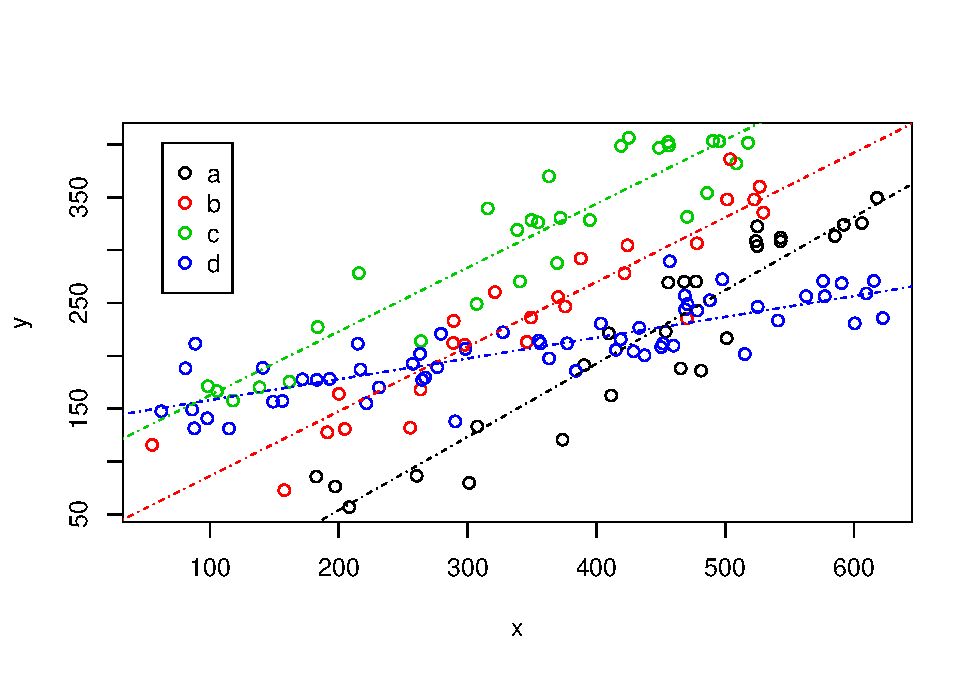
\includegraphics{ECOMODbook_files/figure-latex/unnamed-chunk-56-1.pdf}

Naturally, now the lines do not have the same slope, and we can compare all these in a single plot. This plot is really messy, as it includes the pooled regression (the thick black line), the regressions fitted to independent data sets, one for each museum (the solid lines), and the regressions resulting from the model with museum as a factor covariate (dotted-dashed lines).

\begin{Shaded}
\begin{Highlighting}[]
\CommentTok{#plot all the data}
\KeywordTok{plot}\NormalTok{(y}\OperatorTok{~}\NormalTok{x,}\DataTypeTok{col=}\KeywordTok{as.numeric}\NormalTok{(}\KeywordTok{as.factor}\NormalTok{(z)),}\DataTypeTok{data=}\NormalTok{data4lines,}\DataTypeTok{pch=}\DecValTok{1}\NormalTok{)}
\CommentTok{#completely independet regression lines}
\KeywordTok{abline}\NormalTok{(}\KeywordTok{lm}\NormalTok{(y}\OperatorTok{~}\NormalTok{x,}\DataTypeTok{data=}\NormalTok{data4lines[data4lines}\OperatorTok{$}\NormalTok{z}\OperatorTok{==}\StringTok{"a"}\NormalTok{,]),}\DataTypeTok{col=}\DecValTok{1}\NormalTok{,}\DataTypeTok{lty=}\DecValTok{4}\NormalTok{)}
\KeywordTok{abline}\NormalTok{(}\KeywordTok{lm}\NormalTok{(y}\OperatorTok{~}\NormalTok{x,}\DataTypeTok{data=}\NormalTok{data4lines[data4lines}\OperatorTok{$}\NormalTok{z}\OperatorTok{==}\StringTok{"b"}\NormalTok{,]),}\DataTypeTok{col=}\DecValTok{2}\NormalTok{,}\DataTypeTok{lty=}\DecValTok{4}\NormalTok{)}
\KeywordTok{abline}\NormalTok{(}\KeywordTok{lm}\NormalTok{(y}\OperatorTok{~}\NormalTok{x,}\DataTypeTok{data=}\NormalTok{data4lines[data4lines}\OperatorTok{$}\NormalTok{z}\OperatorTok{==}\StringTok{"c"}\NormalTok{,]),}\DataTypeTok{col=}\DecValTok{3}\NormalTok{,}\DataTypeTok{lty=}\DecValTok{4}\NormalTok{)}
\KeywordTok{abline}\NormalTok{(}\KeywordTok{lm}\NormalTok{(y}\OperatorTok{~}\NormalTok{x,}\DataTypeTok{data=}\NormalTok{data4lines[data4lines}\OperatorTok{$}\NormalTok{z}\OperatorTok{==}\StringTok{"d"}\NormalTok{,]),}\DataTypeTok{col=}\DecValTok{4}\NormalTok{,}\DataTypeTok{lty=}\DecValTok{4}\NormalTok{)}
\CommentTok{#these are the wrong lines... why?}
\KeywordTok{abline}\NormalTok{(lmlinesG,}\DataTypeTok{lwd=}\DecValTok{3}\NormalTok{,}\DataTypeTok{lty=}\DecValTok{2}\NormalTok{)}
\KeywordTok{abline}\NormalTok{(lmlines}\OperatorTok{$}\NormalTok{coefficients[}\DecValTok{1}\NormalTok{],lmlines}\OperatorTok{$}\NormalTok{coefficients[}\DecValTok{2}\NormalTok{],}\DataTypeTok{col=}\DecValTok{1}\NormalTok{)}
\KeywordTok{abline}\NormalTok{(lmlines}\OperatorTok{$}\NormalTok{coefficients[}\DecValTok{1}\NormalTok{]}\OperatorTok{+}\NormalTok{lmlines}\OperatorTok{$}\NormalTok{coefficients[}\DecValTok{3}\NormalTok{],lmlines}\OperatorTok{$}\NormalTok{coefficients[}\DecValTok{2}\NormalTok{],}\DataTypeTok{col=}\DecValTok{2}\NormalTok{)}
\KeywordTok{abline}\NormalTok{(lmlines}\OperatorTok{$}\NormalTok{coefficients[}\DecValTok{1}\NormalTok{]}\OperatorTok{+}\NormalTok{lmlines}\OperatorTok{$}\NormalTok{coefficients[}\DecValTok{4}\NormalTok{],lmlines}\OperatorTok{$}\NormalTok{coefficients[}\DecValTok{2}\NormalTok{],}\DataTypeTok{col=}\DecValTok{3}\NormalTok{)}
\KeywordTok{abline}\NormalTok{(lmlines}\OperatorTok{$}\NormalTok{coefficients[}\DecValTok{1}\NormalTok{]}\OperatorTok{+}\NormalTok{lmlines}\OperatorTok{$}\NormalTok{coefficients[}\DecValTok{5}\NormalTok{],lmlines}\OperatorTok{$}\NormalTok{coefficients[}\DecValTok{2}\NormalTok{],}\DataTypeTok{col=}\DecValTok{4}\NormalTok{)}
\end{Highlighting}
\end{Shaded}

\includegraphics{ECOMODbook_files/figure-latex/unnamed-chunk-57-1.pdf}

But what is the best model to describe the data? That is a mistery that will remain to unfold. For that we will need and additional complication in a regression model: interactions.

But note 1 thing to begin with. The pooled model uses just 2 parameters, one slope and one intercept. The independent lines use 8 parameters, 4 slopes and 4 intercepts, one line for each museum. And the single model with \texttt{lenght} and \texttt{museum} uses 5 parameters, the intercept, the slope for \texttt{length}, and 3 parameters associated with the \(k-1=3\) levels of \texttt{museum} (remember, one level of each factor is absorbed by the regression intercept).

So the choice of what is best might be not straightforward. While we created the data by hand, we do not know the true model! Choosing the best model requires choosing between models with different complexity, i.e.~different number of parameters. We will need a parsimonious model, one that describes the data well, but with a number of parameters that is not too high for the available data. That will also require selection criteria.

Stay tuned for the next episodes on our regression saga!

\hypertarget{aula8}{%
\chapter{Class 8 20 10 2020 - t-test and ANOVA are just linear models}\label{aula8}}

The objective of this chapter is to explore different regression models and to see how they relate to statistical procedures one might not associate with a regression, when in fact, they are just special cases of a regression.

\hypertarget{the-t-test}{%
\section{The t-test}\label{the-t-test}}

While we did not do the t-test in class, this is useful because it allows you to see how a simple t-test is just a linear model too, and acts as a building block for the next examples. The t-test allows us to test the null hypothesis that two samples have the same mean.

Create some data

\begin{Shaded}
\begin{Highlighting}[]
\CommentTok{#Making up a t-test}
\CommentTok{#making sure everyone gets the same results}
\KeywordTok{set.seed}\NormalTok{(}\DecValTok{980}\NormalTok{)}
\end{Highlighting}
\end{Shaded}

Then we define the sample size and the number of treatments

\begin{Shaded}
\begin{Highlighting}[]
\CommentTok{#define sample size}
\NormalTok{n=}\DecValTok{100}
\CommentTok{#define treatments}
\NormalTok{tr=}\KeywordTok{c}\NormalTok{(}\StringTok{"a"}\NormalTok{,}\StringTok{"b"}\NormalTok{)}
\CommentTok{#how many treatments - 2 for a t test}
\NormalTok{ntr=}\KeywordTok{length}\NormalTok{(tr)}
\CommentTok{#balanced design}
\NormalTok{n.by.tr=n}\OperatorTok{/}\NormalTok{ntr}
\end{Highlighting}
\end{Shaded}

Now, we can simulate some data. First, the treatments

\begin{Shaded}
\begin{Highlighting}[]
\NormalTok{type=}\KeywordTok{as.factor}\NormalTok{(}\KeywordTok{rep}\NormalTok{(tr,}\DataTypeTok{each=}\NormalTok{n.by.tr))}
\NormalTok{cores=}\KeywordTok{rep}\NormalTok{(}\DecValTok{1}\OperatorTok{:}\NormalTok{ntr,}\DataTypeTok{each=}\NormalTok{n.by.tr)}
\end{Highlighting}
\end{Shaded}

Then we define the means by treatment - note that they are different, so the null hypothesis in the t-test, that the mean of a is equal to the mean of b, is known to be false in this case.

\begin{Shaded}
\begin{Highlighting}[]
\CommentTok{#define 4 means}
\NormalTok{ms=}\KeywordTok{c}\NormalTok{(}\DecValTok{3}\NormalTok{,}\DecValTok{4}\NormalTok{)}
\end{Highlighting}
\end{Shaded}

Then, the key part, the response variable, with a different mean by treatment. Note the use of the \texttt{ifelse} function, which evaluates its first argument and then assigns the value of its second argument if the first is true or the value of the second if its first argument is false. An example

\begin{Shaded}
\begin{Highlighting}[]
\KeywordTok{ifelse}\NormalTok{(}\DecValTok{3}\OperatorTok{>}\DecValTok{4}\NormalTok{,}\DecValTok{55}\NormalTok{,}\DecValTok{77}\NormalTok{)}
\end{Highlighting}
\end{Shaded}

\begin{verbatim}
## [1] 77
\end{verbatim}

\begin{Shaded}
\begin{Highlighting}[]
\KeywordTok{ifelse}\NormalTok{(}\DecValTok{3}\OperatorTok{<}\DecValTok{4}\NormalTok{,}\DecValTok{55}\NormalTok{,}\DecValTok{77}\NormalTok{)}
\end{Highlighting}
\end{Shaded}

\begin{verbatim}
## [1] 55
\end{verbatim}

So now, generate the response data

\begin{Shaded}
\begin{Highlighting}[]
\NormalTok{ys=}\KeywordTok{ifelse}\NormalTok{(type}\OperatorTok{==}\StringTok{"a"}\NormalTok{,ms[}\DecValTok{1}\NormalTok{],ms[}\DecValTok{2}\NormalTok{])}\OperatorTok{+}\KeywordTok{rnorm}\NormalTok{(n,}\DecValTok{0}\NormalTok{,}\FloatTok{1.5}\NormalTok{)}
\end{Highlighting}
\end{Shaded}

Look at the data

\begin{Shaded}
\begin{Highlighting}[]
\KeywordTok{plot}\NormalTok{(ys}\OperatorTok{~}\NormalTok{type)}
\end{Highlighting}
\end{Shaded}

\includegraphics{ECOMODbook_files/figure-latex/unnamed-chunk-64-1.pdf}

Now, we can run the usual t-test

\begin{Shaded}
\begin{Highlighting}[]
\KeywordTok{t.test}\NormalTok{(ys}\OperatorTok{~}\NormalTok{type)}
\end{Highlighting}
\end{Shaded}

\begin{verbatim}
## 
## 	Welch Two Sample t-test
## 
## data:  ys by type
## t = -2.8043, df = 97.475, p-value = 0.006087
## alternative hypothesis: true difference in means is not equal to 0
## 95 percent confidence interval:
##  -1.4263293 -0.2441277
## sample estimates:
## mean in group a mean in group b 
##        3.106656        3.941884
\end{verbatim}

and now we can do it the linear regression way

\begin{Shaded}
\begin{Highlighting}[]
\NormalTok{lm0=}\KeywordTok{lm}\NormalTok{(ys}\OperatorTok{~}\NormalTok{type)}
\KeywordTok{summary}\NormalTok{(lm0)}
\end{Highlighting}
\end{Shaded}

\begin{verbatim}
## 
## Call:
## lm(formula = ys ~ type)
## 
## Residuals:
##     Min      1Q  Median      3Q     Max 
## -3.1489 -0.9131 -0.1315  1.0295  3.2450 
## 
## Coefficients:
##             Estimate Std. Error t value Pr(>|t|)    
## (Intercept)   3.1067     0.2106  14.751  < 2e-16 ***
## typeb         0.8352     0.2978   2.804  0.00608 ** 
## ---
## Signif. codes:  0 '***' 0.001 '**' 0.01 '*' 0.05 '.' 0.1 ' ' 1
## 
## Residual standard error: 1.489 on 98 degrees of freedom
## Multiple R-squared:  0.07428,	Adjusted R-squared:  0.06484 
## F-statistic: 7.864 on 1 and 98 DF,  p-value: 0.006081
\end{verbatim}

and as you can see, we get the same result for the test statistic. It is the same thing! And we can naturally get the estimated means per group. The mean for a is just the intercept of the model. To get the mean of the group b we add the mean of group b to the intercept, as

\begin{Shaded}
\begin{Highlighting}[]
\CommentTok{#mean of ys under treatment a}
\KeywordTok{summary}\NormalTok{(lm0)}\OperatorTok{$}\NormalTok{coefficients[}\DecValTok{1}\NormalTok{]}
\end{Highlighting}
\end{Shaded}

\begin{verbatim}
## [1] 3.106656
\end{verbatim}

\begin{Shaded}
\begin{Highlighting}[]
\CommentTok{#mean of ys under treatment b}
\KeywordTok{summary}\NormalTok{(lm0)}\OperatorTok{$}\NormalTok{coefficients[}\DecValTok{1}\NormalTok{]}\OperatorTok{+}\NormalTok{lm0}\OperatorTok{$}\NormalTok{coefficients[}\DecValTok{2}\NormalTok{]}
\end{Highlighting}
\end{Shaded}

\begin{verbatim}
##    typeb 
## 3.941884
\end{verbatim}

This is required because in a linear model, all the other parameters associated with levels of a factor will be compared to a reference value, that of the intercept, which happens to be the mean under treatment a. Below you will see more examples of this.

Note we were able to detect the null was false, but this was because we had a decent sample size compared to the variance of the measurements and the magnitude of the true effect (the difference of the means). If we keep the sample size constant but we increase the noise or decrease the magnitude of the difference, we might not get the same result, and make a type II error!

\begin{Shaded}
\begin{Highlighting}[]
\CommentTok{#define 2 means}
\NormalTok{ms=}\KeywordTok{c}\NormalTok{(}\DecValTok{3}\NormalTok{,}\DecValTok{4}\NormalTok{)}
\CommentTok{#increase the variance of the process}
\NormalTok{ys=}\KeywordTok{ifelse}\NormalTok{(type}\OperatorTok{==}\StringTok{"a"}\NormalTok{,ms[}\DecValTok{1}\NormalTok{],ms[}\DecValTok{2}\NormalTok{])}\OperatorTok{+}\KeywordTok{rnorm}\NormalTok{(n,}\DecValTok{0}\NormalTok{,}\DecValTok{5}\NormalTok{)}
\end{Highlighting}
\end{Shaded}

Look at the data, we can see much more variation

\begin{Shaded}
\begin{Highlighting}[]
\KeywordTok{plot}\NormalTok{(ys}\OperatorTok{~}\NormalTok{type)}
\end{Highlighting}
\end{Shaded}

\includegraphics{ECOMODbook_files/figure-latex/unnamed-chunk-69-1.pdf}

Now, we can run the usual t-test

\begin{Shaded}
\begin{Highlighting}[]
\KeywordTok{t.test}\NormalTok{(ys}\OperatorTok{~}\NormalTok{type)}
\end{Highlighting}
\end{Shaded}

\begin{verbatim}
## 
## 	Welch Two Sample t-test
## 
## data:  ys by type
## t = -1.3609, df = 97.949, p-value = 0.1767
## alternative hypothesis: true difference in means is not equal to 0
## 95 percent confidence interval:
##  -3.2822693  0.6118174
## sample estimates:
## mean in group a mean in group b 
##        2.024963        3.360189
\end{verbatim}

and now we can do it the linear regression way

\begin{Shaded}
\begin{Highlighting}[]
\NormalTok{lm0=}\KeywordTok{lm}\NormalTok{(ys}\OperatorTok{~}\NormalTok{type)}
\KeywordTok{summary}\NormalTok{(lm0)}
\end{Highlighting}
\end{Shaded}

\begin{verbatim}
## 
## Call:
## lm(formula = ys ~ type)
## 
## Residuals:
##      Min       1Q   Median       3Q      Max 
## -12.1746  -3.2719   0.2527   3.0578  12.0085 
## 
## Coefficients:
##             Estimate Std. Error t value Pr(>|t|)   
## (Intercept)   2.0250     0.6938   2.919  0.00436 **
## typeb         1.3352     0.9811   1.361  0.17667   
## ---
## Signif. codes:  0 '***' 0.001 '**' 0.01 '*' 0.05 '.' 0.1 ' ' 1
## 
## Residual standard error: 4.906 on 98 degrees of freedom
## Multiple R-squared:  0.01855,	Adjusted R-squared:  0.008533 
## F-statistic: 1.852 on 1 and 98 DF,  p-value: 0.1767
\end{verbatim}

and as you can see, we get the same result for the test statistic, but now with a non significant test.

The same would have happened if we decreased the true difference, while keeping the original magnitude of the error

\begin{Shaded}
\begin{Highlighting}[]
\CommentTok{#define 2 means}
\NormalTok{ms=}\KeywordTok{c}\NormalTok{(}\DecValTok{3}\NormalTok{,}\FloatTok{3.1}\NormalTok{)}
\CommentTok{#increase the variance of the process}
\NormalTok{ys=}\KeywordTok{ifelse}\NormalTok{(type}\OperatorTok{==}\StringTok{"a"}\NormalTok{,ms[}\DecValTok{1}\NormalTok{],ms[}\DecValTok{2}\NormalTok{])}\OperatorTok{+}\KeywordTok{rnorm}\NormalTok{(n,}\DecValTok{0}\NormalTok{,}\FloatTok{1.5}\NormalTok{)}
\end{Highlighting}
\end{Shaded}

Look at the data, we can see again lower variation, but the difference across treatments is very small (so, hard to detect!)

\begin{Shaded}
\begin{Highlighting}[]
\KeywordTok{plot}\NormalTok{(ys}\OperatorTok{~}\NormalTok{type)}
\end{Highlighting}
\end{Shaded}

\includegraphics{ECOMODbook_files/figure-latex/unnamed-chunk-73-1.pdf}

Now, we can run the usual t-test

\begin{Shaded}
\begin{Highlighting}[]
\KeywordTok{t.test}\NormalTok{(ys}\OperatorTok{~}\NormalTok{type)}
\end{Highlighting}
\end{Shaded}

\begin{verbatim}
## 
## 	Welch Two Sample t-test
## 
## data:  ys by type
## t = -0.7994, df = 97.455, p-value = 0.426
## alternative hypothesis: true difference in means is not equal to 0
## 95 percent confidence interval:
##  -0.8149517  0.3469402
## sample estimates:
## mean in group a mean in group b 
##        3.158868        3.392874
\end{verbatim}

and now we can do it the linear regression way

\begin{Shaded}
\begin{Highlighting}[]
\NormalTok{lm0=}\KeywordTok{lm}\NormalTok{(ys}\OperatorTok{~}\NormalTok{type)}
\KeywordTok{summary}\NormalTok{(lm0)}
\end{Highlighting}
\end{Shaded}

\begin{verbatim}
## 
## Call:
## lm(formula = ys ~ type)
## 
## Residuals:
##     Min      1Q  Median      3Q     Max 
## -4.7661 -0.9318  0.0812  0.9087  3.5981 
## 
## Coefficients:
##             Estimate Std. Error t value Pr(>|t|)    
## (Intercept)   3.1589     0.2070  15.261   <2e-16 ***
## typeb         0.2340     0.2927   0.799    0.426    
## ---
## Signif. codes:  0 '***' 0.001 '**' 0.01 '*' 0.05 '.' 0.1 ' ' 1
## 
## Residual standard error: 1.464 on 98 degrees of freedom
## Multiple R-squared:  0.006479,	Adjusted R-squared:  -0.003659 
## F-statistic: 0.639 on 1 and 98 DF,  p-value: 0.426
\end{verbatim}

\hypertarget{anova}{%
\section{ANOVA}\label{anova}}

We move on with perhaps the most famous example of a statistical test/procedure, the ANOVA. An ANOVA is nothing but a linear model, where we have a continuous response variable, which we want to explain as a function of a factor (with several levels, or treatments).

We simulate a data set, beginning by making sure everyone gets the same results by using \texttt{set.seed}

\begin{Shaded}
\begin{Highlighting}[]
\CommentTok{#Making up an ANOVA}
\CommentTok{#An ANOVA}
\CommentTok{#making sure everyone gets the same results}
\KeywordTok{set.seed}\NormalTok{(}\DecValTok{12345}\NormalTok{)}
\end{Highlighting}
\end{Shaded}

Then we define the sample size and the number of treatments

\begin{Shaded}
\begin{Highlighting}[]
\CommentTok{#define sample size}
\NormalTok{n=}\DecValTok{2000}
\CommentTok{#define treatments}
\NormalTok{tr=}\KeywordTok{c}\NormalTok{(}\StringTok{"a"}\NormalTok{,}\StringTok{"b"}\NormalTok{,}\StringTok{"c"}\NormalTok{,}\StringTok{"d"}\NormalTok{)}
\CommentTok{#how many treatments}
\NormalTok{ntr=}\KeywordTok{length}\NormalTok{(tr)}
\CommentTok{#balanced design}
\NormalTok{n.by.tr=n}\OperatorTok{/}\NormalTok{ntr}
\end{Highlighting}
\end{Shaded}

now, we can simulate some data. First, the treatments, but we also generate a independent variable that is not really used for now (\texttt{xs}).

\begin{Shaded}
\begin{Highlighting}[]
\CommentTok{#generate data}
\NormalTok{xs=}\KeywordTok{runif}\NormalTok{(n,}\DecValTok{10}\NormalTok{,}\DecValTok{20}\NormalTok{)}
\NormalTok{type=}\KeywordTok{as.factor}\NormalTok{(}\KeywordTok{rep}\NormalTok{(tr,}\DataTypeTok{each=}\NormalTok{n.by.tr))}
\CommentTok{#if I wanted to recode the levels such that c was the baseline}
\CommentTok{#type=factor(type,levels = c("c","a","b","d"))}
\CommentTok{#get colors for plotting}
\NormalTok{cores=}\KeywordTok{rep}\NormalTok{(}\DecValTok{1}\OperatorTok{:}\NormalTok{ntr,}\DataTypeTok{each=}\NormalTok{n.by.tr)}
\end{Highlighting}
\end{Shaded}

Then we define the means by treatment - note that they are different, so the null hypothesis in an ANOVA, that all the means are the same, is false.

\begin{Shaded}
\begin{Highlighting}[]
\CommentTok{#define 4 means}
\NormalTok{ms=}\KeywordTok{c}\NormalTok{(}\DecValTok{3}\NormalTok{,}\DecValTok{5}\NormalTok{,}\DecValTok{6}\NormalTok{,}\DecValTok{2}\NormalTok{)}
\end{Highlighting}
\end{Shaded}

Then, the key part, the response variable, with a different mean by treatment. Note the use of the \texttt{ifelse} function, which evaluates its first argument and then assigns the value of its second argument if the first is true or the value of the second if its first argument is false. An example

\begin{Shaded}
\begin{Highlighting}[]
\KeywordTok{ifelse}\NormalTok{(}\DecValTok{3}\OperatorTok{>}\DecValTok{4}\NormalTok{,}\DecValTok{55}\NormalTok{,}\DecValTok{77}\NormalTok{)}
\end{Highlighting}
\end{Shaded}

\begin{verbatim}
## [1] 77
\end{verbatim}

\begin{Shaded}
\begin{Highlighting}[]
\KeywordTok{ifelse}\NormalTok{(}\DecValTok{3}\OperatorTok{<}\DecValTok{4}\NormalTok{,}\DecValTok{55}\NormalTok{,}\DecValTok{77}\NormalTok{)}
\end{Highlighting}
\end{Shaded}

\begin{verbatim}
## [1] 55
\end{verbatim}

Note these can be used nested, leading to possible multiple outcomes, and I use that below to define 4 different means depending on the treatment of the observation

\begin{Shaded}
\begin{Highlighting}[]
\KeywordTok{ifelse}\NormalTok{(}\DecValTok{3}\OperatorTok{<}\DecValTok{4}\NormalTok{,}\DecValTok{55}\NormalTok{,}\KeywordTok{ifelse}\NormalTok{(}\DecValTok{3}\OperatorTok{>}\DecValTok{2}\NormalTok{,}\DecValTok{55}\NormalTok{,}\DecValTok{68}\NormalTok{))}
\end{Highlighting}
\end{Shaded}

\begin{verbatim}
## [1] 55
\end{verbatim}

\begin{Shaded}
\begin{Highlighting}[]
\KeywordTok{ifelse}\NormalTok{(}\DecValTok{3}\OperatorTok{>}\DecValTok{4}\NormalTok{,}\DecValTok{55}\NormalTok{,}\KeywordTok{ifelse}\NormalTok{(}\DecValTok{3}\OperatorTok{>}\DecValTok{2}\NormalTok{,}\DecValTok{666}\NormalTok{,}\DecValTok{68}\NormalTok{))}
\end{Highlighting}
\end{Shaded}

\begin{verbatim}
## [1] 666
\end{verbatim}

\begin{Shaded}
\begin{Highlighting}[]
\KeywordTok{ifelse}\NormalTok{(}\DecValTok{3}\OperatorTok{>}\DecValTok{4}\NormalTok{,}\DecValTok{55}\NormalTok{,}\KeywordTok{ifelse}\NormalTok{(}\DecValTok{3}\OperatorTok{<}\DecValTok{2}\NormalTok{,}\DecValTok{666}\NormalTok{,}\DecValTok{68}\NormalTok{))}
\end{Highlighting}
\end{Shaded}

\begin{verbatim}
## [1] 68
\end{verbatim}

So now, generate the data

\begin{Shaded}
\begin{Highlighting}[]
\CommentTok{#ys, not a function of the xs!!!}
\NormalTok{ys=}\KeywordTok{ifelse}\NormalTok{(type}\OperatorTok{==}\StringTok{"a"}\NormalTok{,ms[}\DecValTok{1}\NormalTok{],}\KeywordTok{ifelse}\NormalTok{(type}\OperatorTok{==}\StringTok{"b"}\NormalTok{,ms[}\DecValTok{2}\NormalTok{],}\KeywordTok{ifelse}\NormalTok{(type}\OperatorTok{==}\StringTok{"c"}\NormalTok{,ms[}\DecValTok{3}\NormalTok{],ms[}\DecValTok{4}\NormalTok{])))}\OperatorTok{+}\KeywordTok{rnorm}\NormalTok{(n,}\DecValTok{0}\NormalTok{,}\DecValTok{3}\NormalTok{)}
\end{Highlighting}
\end{Shaded}

We can actually look at the simulated data

\begin{Shaded}
\begin{Highlighting}[]
\KeywordTok{par}\NormalTok{(}\DataTypeTok{mfrow=}\KeywordTok{c}\NormalTok{(}\DecValTok{1}\NormalTok{,}\DecValTok{1}\NormalTok{),}\DataTypeTok{mar=}\KeywordTok{c}\NormalTok{(}\DecValTok{4}\NormalTok{,}\DecValTok{4}\NormalTok{,}\FloatTok{0.5}\NormalTok{,}\FloatTok{0.5}\NormalTok{))}
\KeywordTok{plot}\NormalTok{(ys}\OperatorTok{~}\NormalTok{type,}\DataTypeTok{col=}\DecValTok{1}\OperatorTok{:}\DecValTok{4}\NormalTok{)}
\end{Highlighting}
\end{Shaded}

\includegraphics{ECOMODbook_files/figure-latex/unnamed-chunk-83-1.pdf}

\begin{Shaded}
\begin{Highlighting}[]
\CommentTok{#abline(h=ms,col=1:4)}
\end{Highlighting}
\end{Shaded}

finally, we can implement the linear model and look at its summary

\begin{Shaded}
\begin{Highlighting}[]
\NormalTok{lm.anova=}\KeywordTok{lm}\NormalTok{(ys}\OperatorTok{~}\NormalTok{type)}
\KeywordTok{summary}\NormalTok{(lm.anova)}
\end{Highlighting}
\end{Shaded}

\begin{verbatim}
## 
## Call:
## lm(formula = ys ~ type)
## 
## Residuals:
##     Min      1Q  Median      3Q     Max 
## -9.8735 -2.0115  0.0301  2.0208  9.9976 
## 
## Coefficients:
##             Estimate Std. Error t value Pr(>|t|)    
## (Intercept)   2.8694     0.1319  21.753  < 2e-16 ***
## typeb         2.0788     0.1865  11.143  < 2e-16 ***
## typec         2.9806     0.1865  15.978  < 2e-16 ***
## typed        -0.8726     0.1865  -4.678 3.09e-06 ***
## ---
## Signif. codes:  0 '***' 0.001 '**' 0.01 '*' 0.05 '.' 0.1 ' ' 1
## 
## Residual standard error: 2.95 on 1996 degrees of freedom
## Multiple R-squared:  0.2163,	Adjusted R-squared:  0.2151 
## F-statistic: 183.6 on 3 and 1996 DF,  p-value: < 2.2e-16
\end{verbatim}

note that, again, we can manipulate any sub-components of the created objects

\begin{Shaded}
\begin{Highlighting}[]
\CommentTok{#see the parameters}
\NormalTok{lm.anova}\OperatorTok{$}\NormalTok{coefficients}
\end{Highlighting}
\end{Shaded}

\begin{verbatim}
## (Intercept)       typeb       typec       typed 
##   2.8694412   2.0787628   2.9806367  -0.8726428
\end{verbatim}

\begin{Shaded}
\begin{Highlighting}[]
\CommentTok{#see the third parameter}
\NormalTok{lm.anova}\OperatorTok{$}\NormalTok{coefficients[}\DecValTok{3}\NormalTok{]}
\end{Highlighting}
\end{Shaded}

\begin{verbatim}
##    typec 
## 2.980637
\end{verbatim}

Not surprisingly, because the means were different and we had a large sample size, everything is highly significant. Note that the ANOVA test is actually presented in the regression output, and that is the corresponding F-test

\begin{Shaded}
\begin{Highlighting}[]
\KeywordTok{summary}\NormalTok{(lm.anova)}\OperatorTok{$}\NormalTok{fstatistic}
\end{Highlighting}
\end{Shaded}

\begin{verbatim}
##     value     numdf     dendf 
##  183.6156    3.0000 1996.0000
\end{verbatim}

and we can use the F distribution to calculate the corresponding P-value (note that is already in the output above)

\begin{Shaded}
\begin{Highlighting}[]
\NormalTok{ftest=}\KeywordTok{summary}\NormalTok{(lm.anova)}\OperatorTok{$}\NormalTok{fstatistic[}\DecValTok{1}\NormalTok{]}
\NormalTok{df1=}\KeywordTok{summary}\NormalTok{(lm.anova)}\OperatorTok{$}\NormalTok{fstatistic[}\DecValTok{2}\NormalTok{]}
\NormalTok{df2=}\KeywordTok{summary}\NormalTok{(lm.anova)}\OperatorTok{$}\NormalTok{fstatistic[}\DecValTok{3}\NormalTok{]}
\KeywordTok{pt}\NormalTok{(ftest,df1,df2)}
\end{Highlighting}
\end{Shaded}

\begin{verbatim}
##         value 
## 1.402786e-131
\end{verbatim}

OK, this is actually the exact value, while above the value was reported as just a small value (\textless{} 2.2 \(\times\) 10\(^{-16}\)), but it is the same value, believe me!

Finally, to show (by example) this is just what the ANOVA does, we have the NAOVA itself

\begin{Shaded}
\begin{Highlighting}[]
\KeywordTok{summary}\NormalTok{(}\KeywordTok{aov}\NormalTok{(lm.anova))}
\end{Highlighting}
\end{Shaded}

\begin{verbatim}
##               Df Sum Sq Mean Sq F value Pr(>F)    
## type           3   4792  1597.5   183.6 <2e-16 ***
## Residuals   1996  17365     8.7                   
## ---
## Signif. codes:  0 '***' 0.001 '**' 0.01 '*' 0.05 '.' 0.1 ' ' 1
\end{verbatim}

where everything is the same (test statistic, degrees of freedom and p-values).

Conclusion: an ANOVA is just a special case of a linear model, one where we have a continuous response variable and a factor explanatory covariate. In fact, a two way ANOVA is just the extension where we have a continuous response variable and 2 factor explanatory covariates, and, you guessed it, a three way ANOVA means we have a continuous response variable and a 3 factor explanatory covariates.

Just to finish up this example, we could now plot the true means per treatment, the estimated means per treatment

\begin{Shaded}
\begin{Highlighting}[]
\KeywordTok{par}\NormalTok{(}\DataTypeTok{mfrow=}\KeywordTok{c}\NormalTok{(}\DecValTok{1}\NormalTok{,}\DecValTok{1}\NormalTok{),}\DataTypeTok{mar=}\KeywordTok{c}\NormalTok{(}\DecValTok{4}\NormalTok{,}\DecValTok{4}\NormalTok{,}\FloatTok{0.5}\NormalTok{,}\FloatTok{0.5}\NormalTok{))}
\KeywordTok{plot}\NormalTok{(}\KeywordTok{as.numeric}\NormalTok{(type),ys,}\DataTypeTok{col=}\KeywordTok{as.numeric}\NormalTok{(type),}\DataTypeTok{xlab=}\StringTok{"Treatment"}\NormalTok{,}\DataTypeTok{xaxt=}\StringTok{"n"}\NormalTok{)}
\KeywordTok{axis}\NormalTok{(}\DecValTok{1}\NormalTok{,}\DataTypeTok{at=}\DecValTok{1}\OperatorTok{:}\DecValTok{4}\NormalTok{,letters[}\DecValTok{1}\OperatorTok{:}\DecValTok{4}\NormalTok{])}
\CommentTok{#plot the estimated line for type a}
\KeywordTok{abline}\NormalTok{(}\DataTypeTok{h=}\NormalTok{lm.anova}\OperatorTok{$}\NormalTok{coefficients[}\DecValTok{1}\NormalTok{],}\DataTypeTok{lwd=}\DecValTok{3}\NormalTok{,}\DataTypeTok{col=}\DecValTok{1}\NormalTok{)}
\CommentTok{#plot the mean line for type a}
\KeywordTok{abline}\NormalTok{(}\DataTypeTok{h=}\KeywordTok{mean}\NormalTok{(ys[type}\OperatorTok{==}\StringTok{"a"}\NormalTok{]),}\DataTypeTok{lwd=}\DecValTok{1}\NormalTok{,}\DataTypeTok{col=}\DecValTok{1}\NormalTok{,}\DataTypeTok{lty=}\DecValTok{2}\NormalTok{)}
\CommentTok{#plot the real mean for type a}
\KeywordTok{abline}\NormalTok{(}\DataTypeTok{h=}\NormalTok{ms[}\DecValTok{1}\NormalTok{],}\DataTypeTok{lwd=}\DecValTok{2}\NormalTok{,}\DataTypeTok{col=}\DecValTok{1}\NormalTok{,}\DataTypeTok{lty=}\DecValTok{3}\NormalTok{)}
\CommentTok{#and now for the other types}
\KeywordTok{abline}\NormalTok{(}\DataTypeTok{h=}\NormalTok{lm.anova}\OperatorTok{$}\NormalTok{coefficients[}\DecValTok{1}\NormalTok{]}\OperatorTok{+}\NormalTok{lm.anova}\OperatorTok{$}\NormalTok{coefficients[}\DecValTok{2}\NormalTok{],}\DataTypeTok{lwd=}\DecValTok{3}\NormalTok{,}\DataTypeTok{col=}\DecValTok{2}\NormalTok{)}
\KeywordTok{abline}\NormalTok{(}\DataTypeTok{h=}\KeywordTok{mean}\NormalTok{(ys[type}\OperatorTok{==}\StringTok{"b"}\NormalTok{]),}\DataTypeTok{lwd=}\DecValTok{1}\NormalTok{,}\DataTypeTok{col=}\DecValTok{2}\NormalTok{,}\DataTypeTok{lty=}\DecValTok{2}\NormalTok{)}
\CommentTok{#plot the real mean for type b}
\KeywordTok{abline}\NormalTok{(}\DataTypeTok{h=}\NormalTok{ms[}\DecValTok{2}\NormalTok{],}\DataTypeTok{lwd=}\DecValTok{2}\NormalTok{,}\DataTypeTok{col=}\DecValTok{2}\NormalTok{,}\DataTypeTok{lty=}\DecValTok{3}\NormalTok{)}
\KeywordTok{abline}\NormalTok{(}\DataTypeTok{h=}\NormalTok{lm.anova}\OperatorTok{$}\NormalTok{coefficients[}\DecValTok{1}\NormalTok{]}\OperatorTok{+}\NormalTok{lm.anova}\OperatorTok{$}\NormalTok{coefficients[}\DecValTok{3}\NormalTok{],}\DataTypeTok{lwd=}\DecValTok{3}\NormalTok{,}\DataTypeTok{col=}\DecValTok{3}\NormalTok{)}
\KeywordTok{abline}\NormalTok{(}\DataTypeTok{h=}\KeywordTok{mean}\NormalTok{(ys[type}\OperatorTok{==}\StringTok{"c"}\NormalTok{]),}\DataTypeTok{lwd=}\DecValTok{1}\NormalTok{,}\DataTypeTok{col=}\DecValTok{3}\NormalTok{,}\DataTypeTok{lty=}\DecValTok{2}\NormalTok{)}
\CommentTok{#plot the real mean for type c}
\KeywordTok{abline}\NormalTok{(}\DataTypeTok{h=}\NormalTok{ms[}\DecValTok{3}\NormalTok{],}\DataTypeTok{lwd=}\DecValTok{2}\NormalTok{,}\DataTypeTok{col=}\DecValTok{3}\NormalTok{,}\DataTypeTok{lty=}\DecValTok{3}\NormalTok{)}
\KeywordTok{abline}\NormalTok{(}\DataTypeTok{h=}\NormalTok{lm.anova}\OperatorTok{$}\NormalTok{coefficients[}\DecValTok{1}\NormalTok{]}\OperatorTok{+}\NormalTok{lm.anova}\OperatorTok{$}\NormalTok{coefficients[}\DecValTok{4}\NormalTok{],}\DataTypeTok{lwd=}\DecValTok{3}\NormalTok{,}\DataTypeTok{col=}\DecValTok{4}\NormalTok{)}
\KeywordTok{abline}\NormalTok{(}\DataTypeTok{h=}\KeywordTok{mean}\NormalTok{(ys[type}\OperatorTok{==}\StringTok{"d"}\NormalTok{]),}\DataTypeTok{lwd=}\DecValTok{1}\NormalTok{,}\DataTypeTok{col=}\DecValTok{4}\NormalTok{,}\DataTypeTok{lty=}\DecValTok{2}\NormalTok{)}
\CommentTok{#plot the real mean for type a}
\KeywordTok{abline}\NormalTok{(}\DataTypeTok{h=}\NormalTok{ms[}\DecValTok{4}\NormalTok{],}\DataTypeTok{lwd=}\DecValTok{2}\NormalTok{,}\DataTypeTok{col=}\DecValTok{4}\NormalTok{,}\DataTypeTok{lty=}\DecValTok{3}\NormalTok{)}
\KeywordTok{legend}\NormalTok{(}\StringTok{"topright"}\NormalTok{,}\KeywordTok{c}\NormalTok{(}\StringTok{"Estimated"}\NormalTok{,}\StringTok{"Mean of data"}\NormalTok{,}\StringTok{"True"}\NormalTok{),}\DataTypeTok{lwd=}\KeywordTok{c}\NormalTok{(}\DecValTok{4}\NormalTok{,}\DecValTok{1}\NormalTok{,}\DecValTok{2}\NormalTok{),}\DataTypeTok{lty=}\KeywordTok{c}\NormalTok{(}\DecValTok{1}\NormalTok{,}\DecValTok{3}\NormalTok{,}\DecValTok{2}\NormalTok{),}\DataTypeTok{inset=}\FloatTok{0.03}\NormalTok{)}
\end{Highlighting}
\end{Shaded}

\includegraphics{ECOMODbook_files/figure-latex/unnamed-chunk-89-1.pdf}

It's not easy to see because these overlap (large sample size, high precision) but the estimated means are really close to the real means. It's a bit easier to see if we separate in 4 plots and zoom in on the mean of each treatment, but still the blue lines are all on top of each other, since the mean value was estimated real close to truth (truth=2, estimated = 1.9967984).

\begin{Shaded}
\begin{Highlighting}[]
\CommentTok{#see this in 4 plots, less blur}
\KeywordTok{par}\NormalTok{(}\DataTypeTok{mfrow=}\KeywordTok{c}\NormalTok{(}\DecValTok{2}\NormalTok{,}\DecValTok{2}\NormalTok{),}\DataTypeTok{mar=}\KeywordTok{c}\NormalTok{(}\DecValTok{4}\NormalTok{,}\DecValTok{4}\NormalTok{,}\FloatTok{0.5}\NormalTok{,}\FloatTok{0.5}\NormalTok{))}
\KeywordTok{plot}\NormalTok{(}\KeywordTok{as.numeric}\NormalTok{(type),ys,}\DataTypeTok{col=}\KeywordTok{as.numeric}\NormalTok{(type),}\DataTypeTok{xlab=}\StringTok{"Treatment"}\NormalTok{,}\DataTypeTok{xaxt=}\StringTok{"n"}\NormalTok{,}\DataTypeTok{ylim=}\KeywordTok{mean}\NormalTok{(ys[type}\OperatorTok{==}\StringTok{"a"}\NormalTok{])}\OperatorTok{+}\KeywordTok{c}\NormalTok{(}\OperatorTok{-}\FloatTok{0.5}\NormalTok{,}\FloatTok{0.5}\NormalTok{))}
\KeywordTok{axis}\NormalTok{(}\DecValTok{1}\NormalTok{,}\DataTypeTok{at=}\DecValTok{1}\OperatorTok{:}\DecValTok{4}\NormalTok{,letters[}\DecValTok{1}\OperatorTok{:}\DecValTok{4}\NormalTok{])}
\CommentTok{#plot the estimated line for type a}
\KeywordTok{abline}\NormalTok{(}\DataTypeTok{h=}\NormalTok{lm.anova}\OperatorTok{$}\NormalTok{coefficients[}\DecValTok{1}\NormalTok{],}\DataTypeTok{lwd=}\DecValTok{3}\NormalTok{,}\DataTypeTok{col=}\DecValTok{1}\NormalTok{)}
\CommentTok{#plot the mean line for type a}
\KeywordTok{abline}\NormalTok{(}\DataTypeTok{h=}\KeywordTok{mean}\NormalTok{(ys[type}\OperatorTok{==}\StringTok{"a"}\NormalTok{]),}\DataTypeTok{lwd=}\DecValTok{1}\NormalTok{,}\DataTypeTok{col=}\DecValTok{1}\NormalTok{,}\DataTypeTok{lty=}\DecValTok{2}\NormalTok{)}
\CommentTok{#plot the real mean for type a}
\KeywordTok{abline}\NormalTok{(}\DataTypeTok{h=}\NormalTok{ms[}\DecValTok{1}\NormalTok{],}\DataTypeTok{lwd=}\DecValTok{2}\NormalTok{,}\DataTypeTok{col=}\DecValTok{1}\NormalTok{,}\DataTypeTok{lty=}\DecValTok{3}\NormalTok{)}
\CommentTok{#and now for the other types}
\KeywordTok{plot}\NormalTok{(}\KeywordTok{as.numeric}\NormalTok{(type),ys,}\DataTypeTok{col=}\KeywordTok{as.numeric}\NormalTok{(type),}\DataTypeTok{xlab=}\StringTok{"Treatment"}\NormalTok{,}\DataTypeTok{xaxt=}\StringTok{"n"}\NormalTok{,}\DataTypeTok{ylim=}\KeywordTok{mean}\NormalTok{(ys[type}\OperatorTok{==}\StringTok{"b"}\NormalTok{])}\OperatorTok{+}\KeywordTok{c}\NormalTok{(}\OperatorTok{-}\FloatTok{0.5}\NormalTok{,}\FloatTok{0.5}\NormalTok{))}
\KeywordTok{axis}\NormalTok{(}\DecValTok{1}\NormalTok{,}\DataTypeTok{at=}\DecValTok{1}\OperatorTok{:}\DecValTok{4}\NormalTok{,letters[}\DecValTok{1}\OperatorTok{:}\DecValTok{4}\NormalTok{])}
\KeywordTok{abline}\NormalTok{(}\DataTypeTok{h=}\NormalTok{lm.anova}\OperatorTok{$}\NormalTok{coefficients[}\DecValTok{1}\NormalTok{]}\OperatorTok{+}\NormalTok{lm.anova}\OperatorTok{$}\NormalTok{coefficients[}\DecValTok{2}\NormalTok{],}\DataTypeTok{lwd=}\DecValTok{3}\NormalTok{,}\DataTypeTok{col=}\DecValTok{2}\NormalTok{)}
\KeywordTok{abline}\NormalTok{(}\DataTypeTok{h=}\KeywordTok{mean}\NormalTok{(ys[type}\OperatorTok{==}\StringTok{"b"}\NormalTok{]),}\DataTypeTok{lwd=}\DecValTok{1}\NormalTok{,}\DataTypeTok{col=}\DecValTok{2}\NormalTok{,}\DataTypeTok{lty=}\DecValTok{2}\NormalTok{)}
\CommentTok{#plot the real mean for type b}
\KeywordTok{abline}\NormalTok{(}\DataTypeTok{h=}\NormalTok{ms[}\DecValTok{2}\NormalTok{],}\DataTypeTok{lwd=}\DecValTok{2}\NormalTok{,}\DataTypeTok{col=}\DecValTok{2}\NormalTok{,}\DataTypeTok{lty=}\DecValTok{3}\NormalTok{)}
\KeywordTok{plot}\NormalTok{(}\KeywordTok{as.numeric}\NormalTok{(type),ys,}\DataTypeTok{col=}\KeywordTok{as.numeric}\NormalTok{(type),}\DataTypeTok{xlab=}\StringTok{"Treatment"}\NormalTok{,}\DataTypeTok{xaxt=}\StringTok{"n"}\NormalTok{,}\DataTypeTok{ylim=}\KeywordTok{mean}\NormalTok{(ys[type}\OperatorTok{==}\StringTok{"c"}\NormalTok{])}\OperatorTok{+}\KeywordTok{c}\NormalTok{(}\OperatorTok{-}\FloatTok{0.5}\NormalTok{,}\FloatTok{0.5}\NormalTok{))}
\KeywordTok{axis}\NormalTok{(}\DecValTok{1}\NormalTok{,}\DataTypeTok{at=}\DecValTok{1}\OperatorTok{:}\DecValTok{4}\NormalTok{,letters[}\DecValTok{1}\OperatorTok{:}\DecValTok{4}\NormalTok{])}
\KeywordTok{abline}\NormalTok{(}\DataTypeTok{h=}\NormalTok{lm.anova}\OperatorTok{$}\NormalTok{coefficients[}\DecValTok{1}\NormalTok{]}\OperatorTok{+}\NormalTok{lm.anova}\OperatorTok{$}\NormalTok{coefficients[}\DecValTok{3}\NormalTok{],}\DataTypeTok{lwd=}\DecValTok{3}\NormalTok{,}\DataTypeTok{col=}\DecValTok{3}\NormalTok{)}
\KeywordTok{abline}\NormalTok{(}\DataTypeTok{h=}\KeywordTok{mean}\NormalTok{(ys[type}\OperatorTok{==}\StringTok{"c"}\NormalTok{]),}\DataTypeTok{lwd=}\DecValTok{1}\NormalTok{,}\DataTypeTok{col=}\DecValTok{3}\NormalTok{,}\DataTypeTok{lty=}\DecValTok{2}\NormalTok{)}
\CommentTok{#plot the real mean for type c}
\KeywordTok{abline}\NormalTok{(}\DataTypeTok{h=}\NormalTok{ms[}\DecValTok{3}\NormalTok{],}\DataTypeTok{lwd=}\DecValTok{2}\NormalTok{,}\DataTypeTok{col=}\DecValTok{3}\NormalTok{,}\DataTypeTok{lty=}\DecValTok{3}\NormalTok{)}
\KeywordTok{plot}\NormalTok{(}\KeywordTok{as.numeric}\NormalTok{(type),ys,}\DataTypeTok{col=}\KeywordTok{as.numeric}\NormalTok{(type),}\DataTypeTok{xlab=}\StringTok{"Treatment"}\NormalTok{,}\DataTypeTok{xaxt=}\StringTok{"n"}\NormalTok{,}\DataTypeTok{ylim=}\KeywordTok{mean}\NormalTok{(ys[type}\OperatorTok{==}\StringTok{"d"}\NormalTok{])}\OperatorTok{+}\KeywordTok{c}\NormalTok{(}\OperatorTok{-}\FloatTok{0.5}\NormalTok{,}\FloatTok{0.5}\NormalTok{))}
\KeywordTok{axis}\NormalTok{(}\DecValTok{1}\NormalTok{,}\DataTypeTok{at=}\DecValTok{1}\OperatorTok{:}\DecValTok{4}\NormalTok{,letters[}\DecValTok{1}\OperatorTok{:}\DecValTok{4}\NormalTok{])}
\KeywordTok{abline}\NormalTok{(}\DataTypeTok{h=}\NormalTok{lm.anova}\OperatorTok{$}\NormalTok{coefficients[}\DecValTok{1}\NormalTok{]}\OperatorTok{+}\NormalTok{lm.anova}\OperatorTok{$}\NormalTok{coefficients[}\DecValTok{4}\NormalTok{],}\DataTypeTok{lwd=}\DecValTok{3}\NormalTok{,}\DataTypeTok{col=}\DecValTok{4}\NormalTok{)}
\KeywordTok{abline}\NormalTok{(}\DataTypeTok{h=}\KeywordTok{mean}\NormalTok{(ys[type}\OperatorTok{==}\StringTok{"d"}\NormalTok{]),}\DataTypeTok{lwd=}\DecValTok{1}\NormalTok{,}\DataTypeTok{col=}\DecValTok{4}\NormalTok{,}\DataTypeTok{lty=}\DecValTok{2}\NormalTok{)}
\CommentTok{#plot the real mean for type a}
\KeywordTok{abline}\NormalTok{(}\DataTypeTok{h=}\NormalTok{ms[}\DecValTok{4}\NormalTok{],}\DataTypeTok{lwd=}\DecValTok{2}\NormalTok{,}\DataTypeTok{col=}\DecValTok{4}\NormalTok{,}\DataTypeTok{lty=}\DecValTok{3}\NormalTok{)}
\end{Highlighting}
\end{Shaded}

\includegraphics{ECOMODbook_files/figure-latex/unnamed-chunk-90-1.pdf}

\begin{Shaded}
\begin{Highlighting}[]
\CommentTok{#legend("bottomright",c("Estimated","Mean of data","True"),lwd=c(4,1,2),lty=c(1,3,2),inset=0.05)}
\end{Highlighting}
\end{Shaded}

Now we can check how we can obtain the estimated means from the actual parameters of the regression model (yes, that is what the regression does, it calculates the expected mean of the response, conditional on the treatment).

This is the estimated mean per treatment, using function \texttt{tapply} (very useful function to get any statistics over a variable, inside groups defined by a second variable, here the treatment)

\begin{Shaded}
\begin{Highlighting}[]
\KeywordTok{tapply}\NormalTok{(}\DataTypeTok{X=}\NormalTok{ys,}\DataTypeTok{INDEX=}\NormalTok{type,}\DataTypeTok{FUN=}\NormalTok{mean)}
\end{Highlighting}
\end{Shaded}

\begin{verbatim}
##        a        b        c        d 
## 2.869441 4.948204 5.850078 1.996798
\end{verbatim}

and checking these are obtained from the regression coefficients.
An important note. When you fit models with factors (like here), the intercept term will correspond to the mean of the reference level of the factor(s). Hence, to get the other means, you always have to sum the parameter of the corresponding level to the intercept. So we do it below

\begin{Shaded}
\begin{Highlighting}[]
\CommentTok{#check ANOVA is just computing the mean in each group}
\NormalTok{lm.anova}\OperatorTok{$}\NormalTok{coefficients[}\DecValTok{1}\NormalTok{]}
\end{Highlighting}
\end{Shaded}

\begin{verbatim}
## (Intercept) 
##    2.869441
\end{verbatim}

\begin{Shaded}
\begin{Highlighting}[]
\NormalTok{lm.anova}\OperatorTok{$}\NormalTok{coefficients[}\DecValTok{1}\NormalTok{]}\OperatorTok{+}\NormalTok{lm.anova}\OperatorTok{$}\NormalTok{coefficients[}\DecValTok{2}\NormalTok{]}
\end{Highlighting}
\end{Shaded}

\begin{verbatim}
## (Intercept) 
##    4.948204
\end{verbatim}

\begin{Shaded}
\begin{Highlighting}[]
\NormalTok{lm.anova}\OperatorTok{$}\NormalTok{coefficients[}\DecValTok{1}\NormalTok{]}\OperatorTok{+}\NormalTok{lm.anova}\OperatorTok{$}\NormalTok{coefficients[}\DecValTok{3}\NormalTok{]}
\end{Highlighting}
\end{Shaded}

\begin{verbatim}
## (Intercept) 
##    5.850078
\end{verbatim}

\begin{Shaded}
\begin{Highlighting}[]
\NormalTok{lm.anova}\OperatorTok{$}\NormalTok{coefficients[}\DecValTok{1}\NormalTok{]}\OperatorTok{+}\NormalTok{lm.anova}\OperatorTok{$}\NormalTok{coefficients[}\DecValTok{4}\NormalTok{]}
\end{Highlighting}
\end{Shaded}

\begin{verbatim}
## (Intercept) 
##    1.996798
\end{verbatim}

and we can see these are exactly the same values.

\hypertarget{aula9}{%
\chapter{Class 9: 21 10 2020 - ANCOVA is (also) just a linear model}\label{aula9}}

We move on to Analysis of Covariance, a.k.a. ANCOVA, which is essentially like an ANOVA to which we add a continuous explanatory covariate. The ANCOVA was traditionally used to compare means of an outcome variable between two or more groups taking into account (or to correct for) variability of other variables, called covariates. In other words, ANCOVA allows to compare the adjusted means of two or more independent groups. It's just\ldots{} another linear model with a fancy name! Words adapted from this (looooooooooong!) link \url{https://www.datanovia.com/en/lessons/ancova-in-r/}!

This is an extremely common situation in biology/ecology data. Consider, as an example, you are trying to explain how the weight of a fish depends on its length, but you want to see if that relationship changes per year or site.

Also, remember the dataset we considered in class 7. The data was simulated via this website: \url{https://drawdata.xyz/} and was named \texttt{data4lines.csv}. Those had (about) the same slope in 3 groups, and a different slope in a forth group. That could be analysed as an ANCOVA, and we will look at it that way at the end.

Lets simulate some relevant data and fit the models

\hypertarget{common-slope-different-intercepts-per-treatment}{%
\section{Common slope, different intercepts per treatment}\label{common-slope-different-intercepts-per-treatment}}

We begin with a situation where there are different intercepts per group, but a common slope across all groups. Contrast this with what we saw under the previous class, under chapter \ref{aula8}.

To make it interesting, assume that we are simulating weights for 4 different species, and that weights depend on length (as they almost always do!).

This would be interesting and could be some real data if say one wanted to compare the weights of the fishes of 4 different species, we had captured 50 animals from each species. But we know that the fish lengths across species might be different to begin with, and yet our key interest would be say the weight by species, and in that sense the length was essentially a confounding factor.

\begin{Shaded}
\begin{Highlighting}[]
\CommentTok{#all slopes the same, diferent intercepts - no interactions}
\KeywordTok{set.seed}\NormalTok{(}\DecValTok{1234}\NormalTok{)}
\NormalTok{n<-}\DecValTok{200}
\NormalTok{nbygroup<-}\DecValTok{50}
\NormalTok{xs <-}\StringTok{ }\KeywordTok{runif}\NormalTok{(n,}\DecValTok{10}\NormalTok{,}\DecValTok{20}\NormalTok{)}
\NormalTok{tr <-}\StringTok{ }\KeywordTok{c}\NormalTok{(}\StringTok{"a"}\NormalTok{,}\StringTok{"b"}\NormalTok{,}\StringTok{"c"}\NormalTok{,}\StringTok{"d"}\NormalTok{)}
\NormalTok{type <-}\StringTok{ }\KeywordTok{rep}\NormalTok{(tr,}\DataTypeTok{each=}\NormalTok{nbygroup)}
\NormalTok{cores <-}\StringTok{ }\KeywordTok{rep}\NormalTok{(}\DecValTok{1}\OperatorTok{:}\DecValTok{4}\NormalTok{,}\DataTypeTok{each=}\NormalTok{nbygroup)}
\NormalTok{a<-}\DecValTok{3}
\NormalTok{b<-}\DecValTok{4}
\NormalTok{error<-}\DecValTok{4}
\NormalTok{ys <-}\StringTok{ }\NormalTok{a}\OperatorTok{+}\NormalTok{b}\OperatorTok{*}\NormalTok{xs}\OperatorTok{+}
\KeywordTok{ifelse}\NormalTok{(type}\OperatorTok{==}\StringTok{"a"}\NormalTok{,}\DecValTok{5}\NormalTok{,}\KeywordTok{ifelse}\NormalTok{(type}\OperatorTok{==}\StringTok{"b"}\NormalTok{,}\DecValTok{8}\NormalTok{,}\KeywordTok{ifelse}\NormalTok{(type}\OperatorTok{==}\StringTok{"c"}\NormalTok{,}\DecValTok{10}\NormalTok{,}\DecValTok{12}\NormalTok{)))}\OperatorTok{+}\KeywordTok{rnorm}\NormalTok{(n,}\DecValTok{0}\NormalTok{,}\DecValTok{4}\NormalTok{)}
\end{Highlighting}
\end{Shaded}

We plot the data, all together, per group, and at the end adding the generating line to the plot. It's not easy to make sense of it!

\begin{Shaded}
\begin{Highlighting}[]
\KeywordTok{par}\NormalTok{(}\DataTypeTok{mfrow=}\KeywordTok{c}\NormalTok{(}\DecValTok{2}\NormalTok{,}\DecValTok{3}\NormalTok{),}\DataTypeTok{mar=}\KeywordTok{c}\NormalTok{(}\DecValTok{4}\NormalTok{,}\DecValTok{4}\NormalTok{,}\FloatTok{0.5}\NormalTok{,}\FloatTok{0.5}\NormalTok{))}
\CommentTok{#all the data - uma salganhada!}
\KeywordTok{plot}\NormalTok{(xs,ys,}\DataTypeTok{col=}\NormalTok{cores,}\DataTypeTok{cex=}\FloatTok{0.8}\NormalTok{)}
\CommentTok{#plot the data}
\CommentTok{#par(mfrow=c(2,2),mar=c(4,4,0.5,0.5))}
\KeywordTok{plot}\NormalTok{(xs[type}\OperatorTok{==}\StringTok{"a"}\NormalTok{],ys[type}\OperatorTok{==}\StringTok{"a"}\NormalTok{],}\DataTypeTok{col=}\NormalTok{cores[type}\OperatorTok{==}\StringTok{"a"}\NormalTok{])}
\KeywordTok{abline}\NormalTok{(}\DecValTok{3}\OperatorTok{+}\DecValTok{5}\NormalTok{,}\DecValTok{4}\NormalTok{,}\DataTypeTok{lwd=}\DecValTok{3}\NormalTok{,}\DataTypeTok{col=}\DecValTok{1}\NormalTok{)}
\KeywordTok{plot}\NormalTok{(xs[type}\OperatorTok{==}\StringTok{"b"}\NormalTok{],ys[type}\OperatorTok{==}\StringTok{"b"}\NormalTok{],}\DataTypeTok{col=}\NormalTok{cores[type}\OperatorTok{==}\StringTok{"b"}\NormalTok{])}
\KeywordTok{abline}\NormalTok{(}\DecValTok{3}\OperatorTok{+}\DecValTok{8}\NormalTok{,}\DecValTok{4}\NormalTok{,}\DataTypeTok{lwd=}\DecValTok{3}\NormalTok{,}\DataTypeTok{col=}\DecValTok{2}\NormalTok{)}
\KeywordTok{plot}\NormalTok{(xs[type}\OperatorTok{==}\StringTok{"c"}\NormalTok{],ys[type}\OperatorTok{==}\StringTok{"c"}\NormalTok{],}\DataTypeTok{col=}\NormalTok{cores[type}\OperatorTok{==}\StringTok{"c"}\NormalTok{])}
\KeywordTok{abline}\NormalTok{(}\DecValTok{3}\OperatorTok{+}\DecValTok{10}\NormalTok{,}\DecValTok{4}\NormalTok{,}\DataTypeTok{lwd=}\DecValTok{3}\NormalTok{,}\DataTypeTok{col=}\DecValTok{3}\NormalTok{)}
\KeywordTok{plot}\NormalTok{(xs[type}\OperatorTok{==}\StringTok{"d"}\NormalTok{],ys[type}\OperatorTok{==}\StringTok{"d"}\NormalTok{],}\DataTypeTok{col=}\NormalTok{cores[type}\OperatorTok{==}\StringTok{"d"}\NormalTok{])}
\KeywordTok{abline}\NormalTok{(}\DecValTok{3}\OperatorTok{+}\DecValTok{12}\NormalTok{,}\DecValTok{4}\NormalTok{,}\DataTypeTok{lwd=}\DecValTok{3}\NormalTok{,}\DataTypeTok{col=}\DecValTok{4}\NormalTok{)}
\CommentTok{#the data with each line added to it}
\CommentTok{#par(mfrow=c(1,1),mar=c(4,4,0.5,0.5))}
\KeywordTok{plot}\NormalTok{(xs,ys,}\DataTypeTok{col=}\NormalTok{cores,}\DataTypeTok{cex=}\FloatTok{0.2}\NormalTok{)}
\KeywordTok{abline}\NormalTok{(}\DecValTok{3}\OperatorTok{+}\DecValTok{5}\NormalTok{,}\DecValTok{4}\NormalTok{,}\DataTypeTok{lwd=}\DecValTok{3}\NormalTok{,}\DataTypeTok{col=}\DecValTok{1}\NormalTok{)}
\KeywordTok{abline}\NormalTok{(}\DecValTok{3}\OperatorTok{+}\DecValTok{8}\NormalTok{,}\DecValTok{4}\NormalTok{,}\DataTypeTok{lwd=}\DecValTok{3}\NormalTok{,}\DataTypeTok{col=}\DecValTok{2}\NormalTok{)}
\KeywordTok{abline}\NormalTok{(}\DecValTok{3}\OperatorTok{+}\DecValTok{10}\NormalTok{,}\DecValTok{4}\NormalTok{,}\DataTypeTok{lwd=}\DecValTok{3}\NormalTok{,}\DataTypeTok{col=}\DecValTok{3}\NormalTok{)}
\KeywordTok{abline}\NormalTok{(}\DecValTok{3}\OperatorTok{+}\DecValTok{12}\NormalTok{,}\DecValTok{4}\NormalTok{,}\DataTypeTok{lwd=}\DecValTok{3}\NormalTok{,}\DataTypeTok{col=}\DecValTok{4}\NormalTok{)}
\end{Highlighting}
\end{Shaded}

\includegraphics{ECOMODbook_files/figure-latex/unnamed-chunk-94-1.pdf}

While not the best to look at the data, note that to visually confirm the value of the intercepts we can zoom out on the plot.

\begin{Shaded}
\begin{Highlighting}[]
\KeywordTok{plot}\NormalTok{(xs,ys,}\DataTypeTok{col=}\NormalTok{cores,}\DataTypeTok{xlim=}\KeywordTok{c}\NormalTok{(}\DecValTok{0}\NormalTok{,}\DecValTok{20}\NormalTok{),}\DataTypeTok{ylim=}\KeywordTok{c}\NormalTok{(}\DecValTok{0}\NormalTok{,}\DecValTok{150}\NormalTok{))}
\KeywordTok{abline}\NormalTok{(}\DecValTok{3}\OperatorTok{+}\DecValTok{5}\NormalTok{,}\DecValTok{4}\NormalTok{,}\DataTypeTok{lwd=}\DecValTok{3}\NormalTok{,}\DataTypeTok{col=}\DecValTok{1}\NormalTok{)}
\KeywordTok{abline}\NormalTok{(}\DecValTok{3}\OperatorTok{+}\DecValTok{8}\NormalTok{,}\DecValTok{4}\NormalTok{,}\DataTypeTok{lwd=}\DecValTok{3}\NormalTok{,}\DataTypeTok{col=}\DecValTok{2}\NormalTok{)}
\KeywordTok{abline}\NormalTok{(}\DecValTok{3}\OperatorTok{+}\DecValTok{10}\NormalTok{,}\DecValTok{4}\NormalTok{,}\DataTypeTok{lwd=}\DecValTok{3}\NormalTok{,}\DataTypeTok{col=}\DecValTok{3}\NormalTok{)}
\KeywordTok{abline}\NormalTok{(}\DecValTok{3}\OperatorTok{+}\DecValTok{12}\NormalTok{,}\DecValTok{4}\NormalTok{,}\DataTypeTok{lwd=}\DecValTok{3}\NormalTok{,}\DataTypeTok{col=}\DecValTok{4}\NormalTok{)}
\KeywordTok{abline}\NormalTok{(}\DataTypeTok{h=}\KeywordTok{c}\NormalTok{(}\DecValTok{3}\OperatorTok{+}\DecValTok{5}\NormalTok{,}\DecValTok{3}\OperatorTok{+}\DecValTok{8}\NormalTok{,}\DecValTok{3}\OperatorTok{+}\DecValTok{10}\NormalTok{,}\DecValTok{3}\OperatorTok{+}\DecValTok{12}\NormalTok{),}\DataTypeTok{v=}\DecValTok{0}\NormalTok{,}\DataTypeTok{col=}\KeywordTok{c}\NormalTok{(}\DecValTok{1}\NormalTok{,}\DecValTok{2}\NormalTok{,}\DecValTok{3}\NormalTok{,}\DecValTok{4}\NormalTok{,}\DecValTok{1}\NormalTok{),}\DataTypeTok{lty=}\DecValTok{2}\NormalTok{)}
\end{Highlighting}
\end{Shaded}

\includegraphics{ECOMODbook_files/figure-latex/unnamed-chunk-95-1.pdf}

Now we run the corresponding linear model

\begin{Shaded}
\begin{Highlighting}[]
\CommentTok{#fit the model}
\NormalTok{lm.ancova1 <-}\StringTok{ }\KeywordTok{summary}\NormalTok{(}\KeywordTok{lm}\NormalTok{(ys}\OperatorTok{~}\NormalTok{xs}\OperatorTok{+}\NormalTok{type))}
\NormalTok{lm.ancova1}
\end{Highlighting}
\end{Shaded}

\begin{verbatim}
## 
## Call:
## lm(formula = ys ~ xs + type)
## 
## Residuals:
##      Min       1Q   Median       3Q      Max 
## -13.4694  -2.3640   0.2813   2.1063  11.6596 
## 
## Coefficients:
##             Estimate Std. Error t value Pr(>|t|)    
## (Intercept)  9.24244    1.57462   5.870 1.85e-08 ***
## xs           3.92089    0.09997  39.220  < 2e-16 ***
## typeb        3.11952    0.80410   3.880 0.000143 ***
## typec        5.80393    0.80324   7.226 1.10e-11 ***
## typed        7.36736    0.80434   9.159  < 2e-16 ***
## ---
## Signif. codes:  0 '***' 0.001 '**' 0.01 '*' 0.05 '.' 0.1 ' ' 1
## 
## Residual standard error: 4.008 on 195 degrees of freedom
## Multiple R-squared:  0.9011,	Adjusted R-squared:  0.8991 
## F-statistic: 444.3 on 4 and 195 DF,  p-value: < 2.2e-16
\end{verbatim}

We can check the model intercept coefficients

\begin{Shaded}
\begin{Highlighting}[]
\CommentTok{#estimated values of each intercept}
\NormalTok{lm.ancova1}\OperatorTok{$}\NormalTok{coefficients[}\DecValTok{1}\NormalTok{]}
\end{Highlighting}
\end{Shaded}

\begin{verbatim}
## [1] 9.242444
\end{verbatim}

\begin{Shaded}
\begin{Highlighting}[]
\NormalTok{lm.ancova1}\OperatorTok{$}\NormalTok{coefficients[}\DecValTok{1}\NormalTok{]}\OperatorTok{+}\NormalTok{lm.ancova1}\OperatorTok{$}\NormalTok{coefficients[}\DecValTok{3}\NormalTok{]}
\end{Highlighting}
\end{Shaded}

\begin{verbatim}
## [1] 12.36196
\end{verbatim}

\begin{Shaded}
\begin{Highlighting}[]
\NormalTok{lm.ancova1}\OperatorTok{$}\NormalTok{coefficients[}\DecValTok{1}\NormalTok{]}\OperatorTok{+}\NormalTok{lm.ancova1}\OperatorTok{$}\NormalTok{coefficients[}\DecValTok{4}\NormalTok{]}
\end{Highlighting}
\end{Shaded}

\begin{verbatim}
## [1] 15.04638
\end{verbatim}

\begin{Shaded}
\begin{Highlighting}[]
\NormalTok{lm.ancova1}\OperatorTok{$}\NormalTok{coefficients[}\DecValTok{1}\NormalTok{]}\OperatorTok{+}\NormalTok{lm.ancova1}\OperatorTok{$}\NormalTok{coefficients[}\DecValTok{5}\NormalTok{]}
\end{Highlighting}
\end{Shaded}

\begin{verbatim}
## [1] 16.60981
\end{verbatim}

and the common slope

\begin{Shaded}
\begin{Highlighting}[]
\NormalTok{lm.ancova1}\OperatorTok{$}\NormalTok{coefficients[}\DecValTok{2}\NormalTok{]}
\end{Highlighting}
\end{Shaded}

\begin{verbatim}
## [1] 3.920888
\end{verbatim}

Check how these values are similar (they are estimates) to those we simulated above, slope was 4, and the intercepts were respectively 3+5,3+8,3+10 and 3+12.

We can plot the estimated regression lines

\begin{Shaded}
\begin{Highlighting}[]
\KeywordTok{par}\NormalTok{(}\DataTypeTok{mfrow=}\KeywordTok{c}\NormalTok{(}\DecValTok{1}\NormalTok{,}\DecValTok{1}\NormalTok{),}\DataTypeTok{mar=}\KeywordTok{c}\NormalTok{(}\DecValTok{4}\NormalTok{,}\DecValTok{4}\NormalTok{,}\FloatTok{2.5}\NormalTok{,}\FloatTok{0.5}\NormalTok{))}
\KeywordTok{plot}\NormalTok{(xs,ys,}\DataTypeTok{col=}\NormalTok{cores,}\DataTypeTok{main=}\StringTok{"Estimated regression lines"}\NormalTok{)}
\KeywordTok{abline}\NormalTok{(lm.ancova1}\OperatorTok{$}\NormalTok{coefficients[}\DecValTok{1}\NormalTok{],lm.ancova1}\OperatorTok{$}\NormalTok{coefficients[}\DecValTok{2}\NormalTok{],}\DataTypeTok{col=}\DecValTok{1}\NormalTok{,}\DataTypeTok{lwd=}\DecValTok{2}\NormalTok{)}
\KeywordTok{abline}\NormalTok{(lm.ancova1}\OperatorTok{$}\NormalTok{coefficients[}\DecValTok{1}\NormalTok{]}\OperatorTok{+}\NormalTok{lm.ancova1}\OperatorTok{$}\NormalTok{coefficients[}\DecValTok{3}\NormalTok{],lm.ancova1}\OperatorTok{$}\NormalTok{coefficients[}\DecValTok{2}\NormalTok{],}\DataTypeTok{col=}\DecValTok{2}\NormalTok{,}\DataTypeTok{lwd=}\DecValTok{2}\NormalTok{)}
\KeywordTok{abline}\NormalTok{(lm.ancova1}\OperatorTok{$}\NormalTok{coefficients[}\DecValTok{1}\NormalTok{]}\OperatorTok{+}\NormalTok{lm.ancova1}\OperatorTok{$}\NormalTok{coefficients[}\DecValTok{4}\NormalTok{],lm.ancova1}\OperatorTok{$}\NormalTok{coefficients[}\DecValTok{2}\NormalTok{],}\DataTypeTok{col=}\DecValTok{3}\NormalTok{,}\DataTypeTok{lwd=}\DecValTok{2}\NormalTok{)}

\KeywordTok{abline}\NormalTok{(lm.ancova1}\OperatorTok{$}\NormalTok{coefficients[}\DecValTok{1}\NormalTok{]}\OperatorTok{+}\NormalTok{lm.ancova1}\OperatorTok{$}\NormalTok{coefficients[}\DecValTok{5}\NormalTok{],lm.ancova1}\OperatorTok{$}\NormalTok{coefficients[}\DecValTok{2}\NormalTok{],}\DataTypeTok{col=}\DecValTok{4}\NormalTok{,}\DataTypeTok{lwd=}\DecValTok{2}\NormalTok{)}
\KeywordTok{legend}\NormalTok{(}\StringTok{"topleft"}\NormalTok{,}\DataTypeTok{legend =}\NormalTok{ tr,}\DataTypeTok{lwd=}\DecValTok{2}\NormalTok{,}\DataTypeTok{col=}\DecValTok{1}\OperatorTok{:}\DecValTok{4}\NormalTok{,}\DataTypeTok{inset=}\FloatTok{0.05}\NormalTok{)}
\end{Highlighting}
\end{Shaded}

\includegraphics{ECOMODbook_files/figure-latex/unnamed-chunk-99-1.pdf}

But because we are in a simulation setting, we can contrast the estimated values agaist the reality (the real model).

\begin{Shaded}
\begin{Highlighting}[]
\CommentTok{#In a simulated scenario, we can see we are close to the real values}
\KeywordTok{plot}\NormalTok{(xs,ys,}\DataTypeTok{col=}\NormalTok{cores)}

\CommentTok{#plot the lines}
\KeywordTok{abline}\NormalTok{(a}\OperatorTok{+}\DecValTok{5}\NormalTok{,b,}\DataTypeTok{lwd=}\DecValTok{2}\NormalTok{,}\DataTypeTok{col=}\DecValTok{1}\NormalTok{)}
\KeywordTok{abline}\NormalTok{(a}\OperatorTok{+}\DecValTok{8}\NormalTok{,b,}\DataTypeTok{lwd=}\DecValTok{2}\NormalTok{,}\DataTypeTok{col=}\DecValTok{2}\NormalTok{)}
\KeywordTok{abline}\NormalTok{(a}\OperatorTok{+}\DecValTok{10}\NormalTok{,b,}\DataTypeTok{lwd=}\DecValTok{2}\NormalTok{,}\DataTypeTok{col=}\DecValTok{3}\NormalTok{)}
\KeywordTok{abline}\NormalTok{(a}\OperatorTok{+}\DecValTok{12}\NormalTok{,b,}\DataTypeTok{lwd=}\DecValTok{2}\NormalTok{,}\DataTypeTok{col=}\DecValTok{4}\NormalTok{)}
\CommentTok{#gupo a}
\KeywordTok{abline}\NormalTok{(lm.ancova1}\OperatorTok{$}\NormalTok{coefficients[}\DecValTok{1}\NormalTok{],lm.ancova1}\OperatorTok{$}\NormalTok{coefficients[}\DecValTok{2}\NormalTok{],}\DataTypeTok{lwd=}\DecValTok{1}\NormalTok{,}\DataTypeTok{col=}\DecValTok{1}\NormalTok{,}\DataTypeTok{lty=}\DecValTok{2}\NormalTok{)}
\CommentTok{#grupo b}
\CommentTok{# intercept+slope*xs+intercept especifico do grupo b}
\CommentTok{# (intercept+intercept especifico do grupo b)+ slope}
\KeywordTok{abline}\NormalTok{(lm.ancova1}\OperatorTok{$}\NormalTok{coefficients[}\DecValTok{1}\NormalTok{]}\OperatorTok{+}\NormalTok{lm.ancova1}\OperatorTok{$}\NormalTok{coefficients[}\DecValTok{3}\NormalTok{],lm.ancova1}\OperatorTok{$}\NormalTok{coefficients[}\DecValTok{2}\NormalTok{],}\DataTypeTok{lwd=}\DecValTok{1}\NormalTok{,}\DataTypeTok{col=}\DecValTok{2}\NormalTok{,}\DataTypeTok{lty=}\DecValTok{2}\NormalTok{)}
\CommentTok{#grupo c}
\KeywordTok{abline}\NormalTok{(lm.ancova1}\OperatorTok{$}\NormalTok{coefficients[}\DecValTok{1}\NormalTok{]}\OperatorTok{+}\NormalTok{lm.ancova1}\OperatorTok{$}\NormalTok{coefficients[}\DecValTok{4}\NormalTok{],lm.ancova1}\OperatorTok{$}\NormalTok{coefficients[}\DecValTok{2}\NormalTok{],}\DataTypeTok{lwd=}\DecValTok{1}\NormalTok{,}\DataTypeTok{col=}\DecValTok{3}\NormalTok{,}\DataTypeTok{lty=}\DecValTok{2}\NormalTok{)}
\CommentTok{#grupo d}
\KeywordTok{abline}\NormalTok{(lm.ancova1}\OperatorTok{$}\NormalTok{coefficients[}\DecValTok{1}\NormalTok{]}\OperatorTok{+}\NormalTok{lm.ancova1}\OperatorTok{$}\NormalTok{coefficients[}\DecValTok{5}\NormalTok{],lm.ancova1}\OperatorTok{$}\NormalTok{coefficients[}\DecValTok{2}\NormalTok{],}\DataTypeTok{lwd=}\DecValTok{1}\NormalTok{,}\DataTypeTok{col=}\DecValTok{4}\NormalTok{,}\DataTypeTok{lty=}\DecValTok{2}\NormalTok{)}
\end{Highlighting}
\end{Shaded}

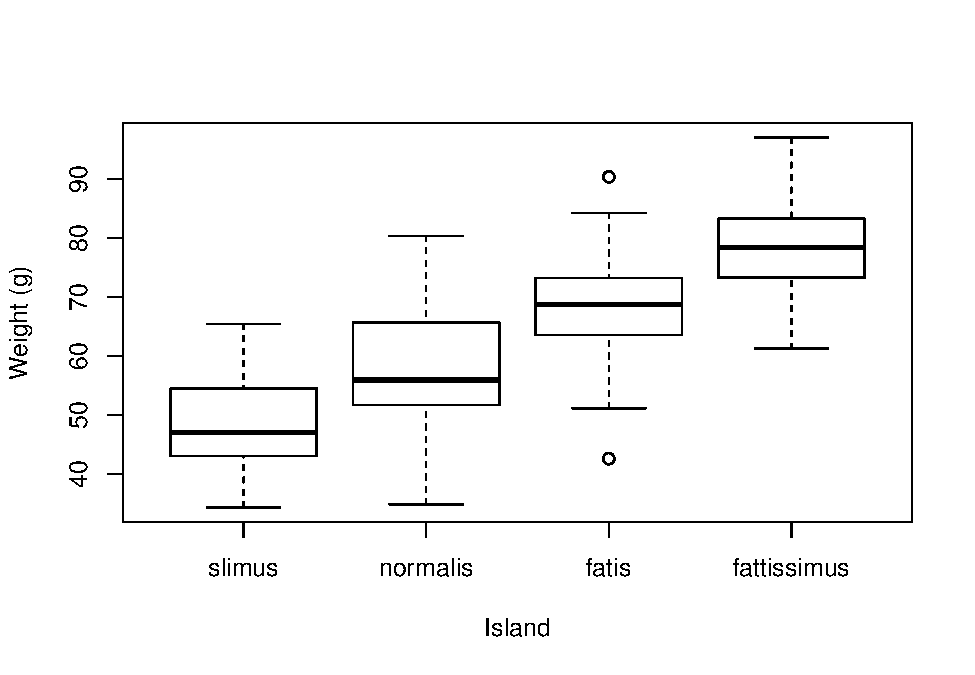
\includegraphics{ECOMODbook_files/figure-latex/unnamed-chunk-100-1.pdf}

As we can see, they are quite close. The error is small compared with the effrect sizes, and the sample size is large enough we can estimate the parameters reasonably well.

But how exactly do we get the predicted intercepts? To understand where they come from we need to see what R does (or, for that matter, what any other software would need to do!) in the background to fit a model with a factor covariate. Remember what the data is

\begin{Shaded}
\begin{Highlighting}[]
\CommentTok{#the data}
\KeywordTok{head}\NormalTok{(}\KeywordTok{data.frame}\NormalTok{(}\DataTypeTok{ys=}\NormalTok{ys,}\DataTypeTok{xs=}\NormalTok{xs,}\DataTypeTok{type=}\NormalTok{type),}\DecValTok{10}\NormalTok{)}
\end{Highlighting}
\end{Shaded}

\begin{verbatim}
##          ys       xs type
## 1  54.20623 11.13703    a
## 2  70.99310 16.22299    a
## 3  72.63496 16.09275    a
## 4  70.92527 16.23379    a
## 5  79.13262 18.60915    a
## 6  74.28038 16.40311    a
## 7  44.79477 10.09496    a
## 8  57.97476 12.32551    a
## 9  76.06322 16.66084    a
## 10 68.36163 15.14251    a
\end{verbatim}

before fitting a factor covariate, we need to replace it by dummy variables (k-1 dummy variables, where k is the number of levels of the factor). Below we look at a set of data lines that allow us to see observations from the diferent \texttt{type}s considered

\begin{Shaded}
\begin{Highlighting}[]
\CommentTok{#explaining it}
\KeywordTok{data.frame}\NormalTok{(}\DataTypeTok{ys=}\NormalTok{ys,}\DataTypeTok{xs=}\NormalTok{xs,}\DataTypeTok{type=}\NormalTok{type,}\DataTypeTok{typeb=}\KeywordTok{ifelse}\NormalTok{(type}\OperatorTok{==}\StringTok{"b"}\NormalTok{,}\DecValTok{1}\NormalTok{,}\DecValTok{0}\NormalTok{),}\DataTypeTok{typec=}\KeywordTok{ifelse}\NormalTok{(type}\OperatorTok{==}\StringTok{"c"}\NormalTok{,}\DecValTok{1}\NormalTok{,}\DecValTok{0}\NormalTok{),}\DataTypeTok{typed=}\KeywordTok{ifelse}\NormalTok{(type}\OperatorTok{==}\StringTok{"d"}\NormalTok{,}\DecValTok{1}\NormalTok{,}\DecValTok{0}\NormalTok{))[}\KeywordTok{c}\NormalTok{(}\DecValTok{1}\NormalTok{,}\DecValTok{49}\NormalTok{,}\DecValTok{50}\NormalTok{,}\DecValTok{51}\NormalTok{,}\DecValTok{99}\NormalTok{,}\DecValTok{100}\NormalTok{,}\DecValTok{101}\NormalTok{,}\DecValTok{149}\NormalTok{,}\DecValTok{150}\NormalTok{,}\DecValTok{151}\NormalTok{,}\DecValTok{200}\NormalTok{),]}
\end{Highlighting}
\end{Shaded}

\begin{verbatim}
##           ys       xs type typeb typec typed
## 1   54.20623 11.13703    a     0     0     0
## 49  59.78224 12.43929    a     0     0     0
## 50  80.00860 17.65460    a     0     0     0
## 51  52.44224 10.73780    b     1     0     0
## 99  64.03652 13.09647    b     1     0     0
## 100 72.37184 17.42120    b     1     0     0
## 101 56.35918 10.35457    c     0     1     0
## 149 93.28892 19.80787    c     0     1     0
## 150 77.14469 15.76813    c     0     1     0
## 151 74.30940 14.39042    d     0     0     1
## 200 81.84481 16.39205    d     0     0     1
\end{verbatim}

So R first builds what is known as the design matrix. Notation wise Y= parameters \(\times\) design matrix, or Y = \(\beta\)X (see e.g.~\url{https://en.wikipedia.org/wiki/Design_matrix})

\begin{Shaded}
\begin{Highlighting}[]
\CommentTok{#the design matrix}
\KeywordTok{head}\NormalTok{(}\KeywordTok{data.frame}\NormalTok{(}\DataTypeTok{xs=}\NormalTok{xs,}\DataTypeTok{typeb=}\KeywordTok{ifelse}\NormalTok{(type}\OperatorTok{==}\StringTok{"b"}\NormalTok{,}\DecValTok{1}\NormalTok{,}\DecValTok{0}\NormalTok{),}\DataTypeTok{typec=}\KeywordTok{ifelse}\NormalTok{(type}\OperatorTok{==}\StringTok{"c"}\NormalTok{,}\DecValTok{1}\NormalTok{,}\DecValTok{0}\NormalTok{),}\DataTypeTok{typed=}\KeywordTok{ifelse}\NormalTok{(type}\OperatorTok{==}\StringTok{"d"}\NormalTok{,}\DecValTok{1}\NormalTok{,}\DecValTok{0}\NormalTok{)))}
\end{Highlighting}
\end{Shaded}

\begin{verbatim}
##         xs typeb typec typed
## 1 11.13703     0     0     0
## 2 16.22299     0     0     0
## 3 16.09275     0     0     0
## 4 16.23379     0     0     0
## 5 18.60915     0     0     0
## 6 16.40311     0     0     0
\end{verbatim}

and that is what it uses for the fitting. Therefore, if we want to know the intercept of say \texttt{type} c, we need to sum the common intercept with the parameter associates with the dummy variable \texttt{typeb}.

This would be an ANCOVA, and here we would conclude that the mean of the response was different for the different levels of \(z\) , once accounting for the fact that the \(xs\) varied. this is evident since all the coefficients estimates and associated precisions in the summary of the model above would lead to rejecting the null hypothesis that their value was 0, as can be seen by the corresponding very small p-values. Not a surprise, since we simulated them as different and the errors were small.

Taks: Increase the simulated error or lower the coefficients until you get type II errors. Change also sample sizes and effect sizes to see the impacts on the model performance!

\hypertarget{aula10}{%
\chapter{Class 10: 27 10 2020}\label{aula10}}

In class 10 we actually had Miguel Pais talking about Individual Based Models.

In this chapter we look again at the ANCOVA model presented in chapter \ref{aula9}, but under a different perspective. I decided to create this material as a bonus for students, to understand why the ANCOVA is what it is. As a bonus, this also provides a cautionary tale about the dangers of non-random sampling, or more generally, confounding due to unmeasured factors that might affect our response variable.

Therefore,

\hypertarget{same-story-another-spin}{%
\section{Same story, another spin}\label{same-story-another-spin}}

As we noted above, the ANCOVA would be an useful model to compare means of an outcome variable between two or more groups taking into account (or to correct for) variability of other variables, often called covariates. In other words, ANCOVA allows to compare the adjusted means of two or more independent groups.

Here we tell the same story from chapter \ref{aula9} under said perspective. We will do so with the help of two unlikely caracters. This is the story of two friends: a biologist that is exploring the weights of lizards, and his friend, a former biology that decided to take an MSc in Ecological Statistics!

The biologist will be the hero of our story. He has a great name. George Ramsey Ernest Armitage Turner. Note that he has 5 names, unusal in the Anglosaxonic world, but not that uncommon is say Portugal. To make it easier, we'll call him just by his initials. So\ldots{} let's call him Great :) Great's fried, who's a great friend, is simply called John. Boring, but hey, names aren't something you can choose are they, and when you are just the sidekick on the story, you can't complain!

Great when on a journey to a distant archipelago where there are 4 islands, each potentially with a different species of lizard that Great is interested in. The folks providing names to islands where not has imaginative as Great's parents, so the islands are called just A, B, C and D. Imagine that Great did a great job and collected a great sample of lizards in each island. Great is alos interested in the amount of insects available for the lizards in each of the islands. He thinks they might determine the weight of the lizards. Weight is related to condition, condition to fecundity and survival, and so on.

Imagine Great wanted to compare the weights of lizard specimens he collected in each of the 4 islands. He happen to capture a number of animals in each island, and we will label them as A to D, as per the islands.

(note, since this is a story, this time I am not showing you how the data was created (=simulated), for narrative reasons!)

Great ploted the weights, in grams (g), of the captured lizards. These look like this:

\begin{Shaded}
\begin{Highlighting}[]
\KeywordTok{hist}\NormalTok{(ys,}\DataTypeTok{main=}\StringTok{"Lizards pooled across 4 islands"}\NormalTok{,}\DataTypeTok{xlab=}\StringTok{"Weight (g)"}\NormalTok{)}
\end{Highlighting}
\end{Shaded}

\includegraphics{ECOMODbook_files/figure-latex/unnamed-chunk-105-1.pdf}

The distribution is unimodal and about simetrical. When lizards are separated by island, they look like this

\begin{Shaded}
\begin{Highlighting}[]
\KeywordTok{boxplot}\NormalTok{(ys}\OperatorTok{~}\NormalTok{type,}\DataTypeTok{ylab=}\StringTok{"Weight (g)"}\NormalTok{,}\DataTypeTok{xlab=}\StringTok{"Island"}\NormalTok{)}
\end{Highlighting}
\end{Shaded}

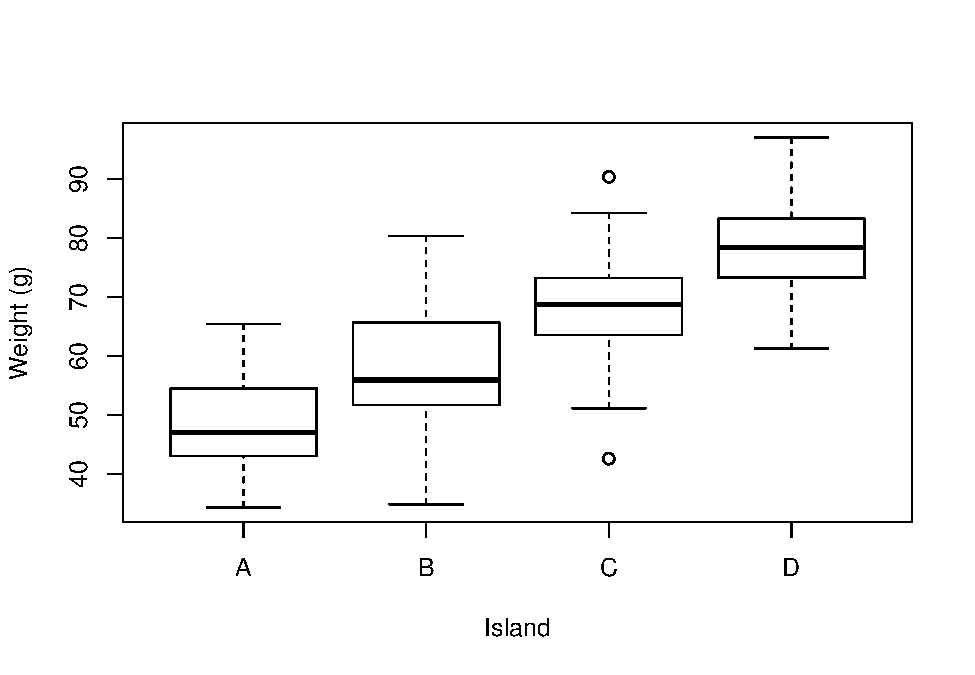
\includegraphics{ECOMODbook_files/figure-latex/unnamed-chunk-106-1.pdf}

There seem to be clear differences in the weights per species, as a standard linear model (e.g.~an ANOVA, see \ref{aula8}) will show:

\begin{Shaded}
\begin{Highlighting}[]
\KeywordTok{summary}\NormalTok{(}\KeywordTok{lm}\NormalTok{(ys}\OperatorTok{~}\NormalTok{type))}
\end{Highlighting}
\end{Shaded}

\begin{verbatim}
## 
## Call:
## lm(formula = ys ~ type)
## 
## Residuals:
##      Min       1Q   Median       3Q      Max 
## -25.7066  -5.3458  -0.5474   6.2330  22.9767 
## 
## Coefficients:
##             Estimate Std. Error t value Pr(>|t|)    
## (Intercept)   48.079      1.199  40.105  < 2e-16 ***
## typeB          9.305      1.695   5.489 1.24e-07 ***
## typeC         20.254      1.695  11.947  < 2e-16 ***
## typeD         30.583      1.695  18.039  < 2e-16 ***
## ---
## Signif. codes:  0 '***' 0.001 '**' 0.01 '*' 0.05 '.' 0.1 ' ' 1
## 
## Residual standard error: 8.477 on 196 degrees of freedom
## Multiple R-squared:  0.652,	Adjusted R-squared:  0.6467 
## F-statistic: 122.4 on 3 and 196 DF,  p-value: < 2.2e-16
\end{verbatim}

Great is happy, he had seen differents amounts of insects in each island and so he is already thinking about a paper he will write about how the size of the lizards depends on food availability.

Further, he just had a great thought. He calls these GGTs: Great great thoughts. He is thinking about proposing that these correspond to different species in each island, and he is already dreaming about the names of his new species: he is considering naming them ``slimus'', ``normalis'', ``fatis'', ``fattissimus'', for animals in islands A, B, C and D, respectively. The plot would then read just like this, which looks\ldots{} you guessed it\ldots{} great.

\begin{Shaded}
\begin{Highlighting}[]
\NormalTok{spnames <-}\StringTok{ }\KeywordTok{c}\NormalTok{(}\StringTok{"slimus"}\NormalTok{, }\StringTok{"normalis"}\NormalTok{, }\StringTok{"fatis"}\NormalTok{, }\StringTok{"fattissimus"}\NormalTok{)}
\KeywordTok{boxplot}\NormalTok{(ys}\OperatorTok{~}\NormalTok{type,}\DataTypeTok{ylab=}\StringTok{"Weight (g)"}\NormalTok{,}\DataTypeTok{xlab=}\StringTok{"Island"}\NormalTok{,}
\DataTypeTok{names=}\NormalTok{spnames)}
\end{Highlighting}
\end{Shaded}

\includegraphics{ECOMODbook_files/figure-latex/unnamed-chunk-108-1.pdf}

Unfortunately, he goes to the pub and tells John about his findings. John has been doing some modelling courses at the Univeristy and is very interested about sampling.
John asks Great a great set of questions: ``How did you selected the lizards you captured? What about the lengths of the lizards? Were the animals from each island of about the same length? In other words, did you control the weights for length? Because longer animals will generaly heavier, you know?''

Great had not thought about that yet, indeed. He's feeling dizzy, might be the beers he had, might be the questions he was just asked! He rushes home and looks at the data. And in fact, the different lizards from the different islands have very different lengths to begin with, as we can see in the plot below.

\begin{Shaded}
\begin{Highlighting}[]
\KeywordTok{boxplot}\NormalTok{(xs}\OperatorTok{~}\NormalTok{type,}\DataTypeTok{ylab=}\StringTok{"Length"}\NormalTok{,}\DataTypeTok{xlab=}\StringTok{"Species"}\NormalTok{)}
\end{Highlighting}
\end{Shaded}

\includegraphics{ECOMODbook_files/figure-latex/unnamed-chunk-109-1.pdf}

\begin{Shaded}
\begin{Highlighting}[]
\KeywordTok{summary}\NormalTok{(}\KeywordTok{lm}\NormalTok{(xs}\OperatorTok{~}\NormalTok{type))}
\end{Highlighting}
\end{Shaded}

\begin{verbatim}
## 
## Call:
## lm(formula = xs ~ type)
## 
## Residuals:
##      Min       1Q   Median       3Q      Max 
## -1.30243 -0.60977 -0.06891  0.52388  1.41528 
## 
## Coefficients:
##             Estimate Std. Error t value Pr(>|t|)    
## (Intercept)  11.2298     0.1034  108.55   <2e-16 ***
## typeB         2.2413     0.1463   15.32   <2e-16 ***
## typeC         4.6822     0.1463   32.00   <2e-16 ***
## typeD         7.4886     0.1463   51.19   <2e-16 ***
## ---
## Signif. codes:  0 '***' 0.001 '**' 0.01 '*' 0.05 '.' 0.1 ' ' 1
## 
## Residual standard error: 0.7315 on 196 degrees of freedom
## Multiple R-squared:  0.9368,	Adjusted R-squared:  0.9358 
## F-statistic: 968.6 on 3 and 196 DF,  p-value: < 2.2e-16
\end{verbatim}

In his mind Great has a vague memory of a teacher in Numerical Ecology that one should explore the data before modelling. He would have avoided this embarassement if he only had done that. Before leaving the pub he heard John saying he should look into ANCOVA's. Something about ``you need to test for the weights, accounting for differences in lengths!''.

He goes into his books and finds that ANCOVA is just a linear model, where you model a response (weight, he realizes) with a factor (island) and a continous variable (lenght).

He implements the models and, much to his despair, realizes that, once he you accounts for the length, the weights are not different per island. The damn lizards are exactly the same weight in the different islands once you account for their length\ldots{} :(

\begin{Shaded}
\begin{Highlighting}[]
\KeywordTok{summary}\NormalTok{(}\KeywordTok{lm}\NormalTok{(ys}\OperatorTok{~}\NormalTok{xs}\OperatorTok{+}\NormalTok{type))}
\end{Highlighting}
\end{Shaded}

\begin{verbatim}
## 
## Call:
## lm(formula = ys ~ xs + type)
## 
## Residuals:
##      Min       1Q   Median       3Q      Max 
## -27.4613  -4.7367   0.5201   4.2655  23.8079 
## 
## Coefficients:
##             Estimate Std. Error t value Pr(>|t|)    
## (Intercept)   5.3307     8.8751   0.601    0.549    
## xs            3.8067     0.7838   4.857 2.45e-06 ***
## typeB         0.7735     2.3798   0.325    0.746    
## typeC         2.4305     4.0058   0.607    0.545    
## typeD         2.0764     6.0853   0.341    0.733    
## ---
## Signif. codes:  0 '***' 0.001 '**' 0.01 '*' 0.05 '.' 0.1 ' ' 1
## 
## Residual standard error: 8.027 on 195 degrees of freedom
## Multiple R-squared:  0.6896,	Adjusted R-squared:  0.6832 
## F-statistic: 108.3 on 4 and 195 DF,  p-value: < 2.2e-16
\end{verbatim}

He sees his paper further and further farther away. This is what we saw: the same line explains all the data, irrespectively of group. In other words, there is not a different relationship per species between weight and length! His great ecologycal theory goes to the bin!

\begin{Shaded}
\begin{Highlighting}[]
\KeywordTok{plot}\NormalTok{(ys}\OperatorTok{~}\NormalTok{xs,}\DataTypeTok{col=}\NormalTok{cores)}
\KeywordTok{abline}\NormalTok{(a,b,}\DataTypeTok{lwd=}\DecValTok{3}\NormalTok{,}\DataTypeTok{lty=}\DecValTok{2}\NormalTok{)}
\end{Highlighting}
\end{Shaded}

\includegraphics{ECOMODbook_files/figure-latex/unnamed-chunk-111-1.pdf}

Now, that is dismaying, but interesting. So Great returns to the pub and he asks John: ``Would the oposite be possible? Say things looked just the same, yet they were different after accounting for a confounding factor?''.

``Yes'', John replied: ``I have heard about that situation, but have never seen it in a real data set before. Of course that is hard to happen, because \emph{the stars need to align}. But it can happen in theory. Imagine the situation where the relationship between length and weight is different per group. However, out of a strange confounding circumstance, the observed weights happen to be similar, because we sampled (just the right, in this case, wrong!) different lengthts in each species.''

By now Great has a great headache, but he wants to see this with his own eyes, so he goes back home, sits in front of the computer, opens R and decides: ``I will simulate this example''. That is what we will do here.

Imagine the following example:

The lizards relationship between weight and length is different per island. Say, akin to what we saw before. Just by magin, we have access to all the lizards in the island.

\begin{Shaded}
\begin{Highlighting}[]
\CommentTok{#all slopes the same, diferent intercepts - no interactions}
\KeywordTok{set.seed}\NormalTok{(}\DecValTok{12345}\NormalTok{)}
\NormalTok{n<-}\DecValTok{2000}
\NormalTok{nbygroup<-}\DecValTok{500}
\NormalTok{xs <-}\StringTok{ }\KeywordTok{runif}\NormalTok{(n,}\DecValTok{10}\NormalTok{,}\DecValTok{20}\NormalTok{)}
\NormalTok{island <-}\StringTok{ }\KeywordTok{c}\NormalTok{(}\StringTok{"A"}\NormalTok{,}\StringTok{"B"}\NormalTok{,}\StringTok{"C"}\NormalTok{,}\StringTok{"D"}\NormalTok{)}
\NormalTok{type <-}\StringTok{ }\KeywordTok{rep}\NormalTok{(island,}\DataTypeTok{each=}\NormalTok{nbygroup)}
\NormalTok{cores <-}\StringTok{ }\KeywordTok{rep}\NormalTok{(}\DecValTok{1}\OperatorTok{:}\DecValTok{4}\NormalTok{,}\DataTypeTok{each=}\NormalTok{nbygroup)}
\NormalTok{a<-}\DecValTok{12}
\NormalTok{b<-}\DecValTok{4}
\NormalTok{error<-}\DecValTok{4}
\NormalTok{ys <-}\StringTok{ }\NormalTok{a}\OperatorTok{+}\NormalTok{b}\OperatorTok{*}\NormalTok{xs}\OperatorTok{+}
\KeywordTok{ifelse}\NormalTok{(type}\OperatorTok{==}\StringTok{"A"}\NormalTok{,}\DecValTok{5}\NormalTok{,}\KeywordTok{ifelse}\NormalTok{(type}\OperatorTok{==}\StringTok{"B"}\NormalTok{,}\DecValTok{12}\NormalTok{,}\KeywordTok{ifelse}\NormalTok{(type}\OperatorTok{==}\StringTok{"C"}\NormalTok{,}\DecValTok{18}\NormalTok{,}\DecValTok{22}\NormalTok{)))}\OperatorTok{+}\KeywordTok{rnorm}\NormalTok{(n,}\DecValTok{0}\NormalTok{,}\DecValTok{4}\NormalTok{)}
\KeywordTok{plot}\NormalTok{(xs,ys,}\DataTypeTok{col=}\NormalTok{cores)}
\KeywordTok{abline}\NormalTok{(}\DecValTok{12}\OperatorTok{+}\DecValTok{5}\NormalTok{,}\DecValTok{4}\NormalTok{,}\DataTypeTok{lwd=}\DecValTok{3}\NormalTok{,}\DataTypeTok{col=}\DecValTok{1}\NormalTok{)}
\KeywordTok{abline}\NormalTok{(}\DecValTok{12}\OperatorTok{+}\DecValTok{12}\NormalTok{,}\DecValTok{4}\NormalTok{,}\DataTypeTok{lwd=}\DecValTok{3}\NormalTok{,}\DataTypeTok{col=}\DecValTok{2}\NormalTok{)}
\KeywordTok{abline}\NormalTok{(}\DecValTok{12}\OperatorTok{+}\DecValTok{18}\NormalTok{,}\DecValTok{4}\NormalTok{,}\DataTypeTok{lwd=}\DecValTok{3}\NormalTok{,}\DataTypeTok{col=}\DecValTok{3}\NormalTok{)}
\KeywordTok{abline}\NormalTok{(}\DecValTok{12}\OperatorTok{+}\DecValTok{22}\NormalTok{,}\DecValTok{4}\NormalTok{,}\DataTypeTok{lwd=}\DecValTok{3}\NormalTok{,}\DataTypeTok{col=}\DecValTok{4}\NormalTok{)}
\end{Highlighting}
\end{Shaded}

\includegraphics{ECOMODbook_files/figure-latex/unnamed-chunk-112-1.pdf}

Now imagine, for the sake of argument, that in all islands we captured lizards with lengths spanning about 2 cm, but in island A we caught animals with about 18 cm, in B with about 16 cm, in c with about 15 cm and in D with about 14 cm, on average. We can simulate that non-random sampling process with respect to lenghth.

\begin{Shaded}
\begin{Highlighting}[]
\NormalTok{sampled.a<-}\KeywordTok{which}\NormalTok{(xs}\OperatorTok{>}\DecValTok{17} \OperatorTok{&}\StringTok{ }\NormalTok{xs}\OperatorTok{<}\DecValTok{19} \OperatorTok{&}\StringTok{ }\NormalTok{type}\OperatorTok{==}\StringTok{"A"}\NormalTok{)}
\NormalTok{sampled.b<-}\KeywordTok{which}\NormalTok{(xs}\OperatorTok{>}\DecValTok{15} \OperatorTok{&}\StringTok{ }\NormalTok{xs}\OperatorTok{<}\DecValTok{17} \OperatorTok{&}\StringTok{ }\NormalTok{type}\OperatorTok{==}\StringTok{"B"}\NormalTok{)}
\NormalTok{sampled.c<-}\KeywordTok{which}\NormalTok{(xs}\OperatorTok{>}\DecValTok{14} \OperatorTok{&}\StringTok{ }\NormalTok{xs}\OperatorTok{<}\DecValTok{16} \OperatorTok{&}\StringTok{ }\NormalTok{type}\OperatorTok{==}\StringTok{"C"}\NormalTok{)}
\NormalTok{sampled.d<-}\KeywordTok{which}\NormalTok{(xs}\OperatorTok{>}\DecValTok{13} \OperatorTok{&}\StringTok{ }\NormalTok{xs}\OperatorTok{<}\DecValTok{15} \OperatorTok{&}\StringTok{ }\NormalTok{type}\OperatorTok{==}\StringTok{"D"}\NormalTok{)}
\NormalTok{sample.all<-}\KeywordTok{c}\NormalTok{(sampled.a,sampled.b,sampled.c,sampled.d)}
\CommentTok{#select a biased sample!}
\NormalTok{xs2<-xs[sample.all]}
\NormalTok{ys2<-ys[sample.all]}
\NormalTok{type2<-type[sample.all]}
\NormalTok{cores2<-cores[sample.all]}
\KeywordTok{table}\NormalTok{(type2)}
\end{Highlighting}
\end{Shaded}

\begin{verbatim}
## type2
##   A   B   C   D 
## 119 116 108 100
\end{verbatim}

Now, if this is our sample, what happens when we look at the weights alone? First, let's look at the previous plot with the sampled data highlighted in colors and the non sampled data greyed out.

\begin{Shaded}
\begin{Highlighting}[]
\KeywordTok{plot}\NormalTok{(xs,ys,}\DataTypeTok{pch=}\StringTok{"."}\NormalTok{,}\DataTypeTok{col=}\StringTok{"grey"}\NormalTok{)}
\KeywordTok{points}\NormalTok{(xs2,ys2,}\DataTypeTok{col=}\NormalTok{cores2,}\DataTypeTok{cex=}\FloatTok{0.5}\NormalTok{)}
\end{Highlighting}
\end{Shaded}

\includegraphics{ECOMODbook_files/figure-latex/unnamed-chunk-114-1.pdf}

\begin{Shaded}
\begin{Highlighting}[]
\CommentTok{#abline(12+5,4,lwd=3,col=1)}
\CommentTok{#abline(12+12,4,lwd=3,col=2)}
\CommentTok{#abline(12+18,4,lwd=3,col=3)}
\CommentTok{#abline(12+22,4,lwd=3,col=4)}
\end{Highlighting}
\end{Shaded}

That was really not a random sample. And non-random samples always ask for trouble. Lets see what happens here. If we look at weights per island, there seems to be no effect:

\begin{Shaded}
\begin{Highlighting}[]
\KeywordTok{boxplot}\NormalTok{(ys2}\OperatorTok{~}\NormalTok{type2)}
\end{Highlighting}
\end{Shaded}

\includegraphics{ECOMODbook_files/figure-latex/unnamed-chunk-115-1.pdf}

If we test formally for it with an ANOVA, it seems like there is absolutely no effect of weight:

\begin{Shaded}
\begin{Highlighting}[]
\KeywordTok{summary}\NormalTok{(}\KeywordTok{lm}\NormalTok{(ys2}\OperatorTok{~}\NormalTok{type2))}
\end{Highlighting}
\end{Shaded}

\begin{verbatim}
## 
## Call:
## lm(formula = ys2 ~ type2)
## 
## Residuals:
##     Min      1Q  Median      3Q     Max 
## -13.918  -3.137   0.035   3.142  13.648 
## 
## Coefficients:
##             Estimate Std. Error t value Pr(>|t|)    
## (Intercept)  88.9384     0.4194 212.040   <2e-16 ***
## type2B       -0.4589     0.5970  -0.769    0.443    
## type2C        0.4200     0.6081   0.691    0.490    
## type2D        0.7764     0.6207   1.251    0.212    
## ---
## Signif. codes:  0 '***' 0.001 '**' 0.01 '*' 0.05 '.' 0.1 ' ' 1
## 
## Residual standard error: 4.576 on 439 degrees of freedom
## Multiple R-squared:  0.009992,	Adjusted R-squared:  0.003227 
## F-statistic: 1.477 on 3 and 439 DF,  p-value: 0.2201
\end{verbatim}

This is where we need to be smart. If we conducts the correct analysis, one that includes and adjusts for the effect of length, the differences in length to weight relationship are clear. The intercepts of the different lines are all different from each other.

\begin{Shaded}
\begin{Highlighting}[]
\KeywordTok{summary}\NormalTok{(}\KeywordTok{lm}\NormalTok{(ys2}\OperatorTok{~}\NormalTok{type2}\OperatorTok{+}\NormalTok{xs2))}
\end{Highlighting}
\end{Shaded}

\begin{verbatim}
## 
## Call:
## lm(formula = ys2 ~ type2 + xs2)
## 
## Residuals:
##      Min       1Q   Median       3Q      Max 
## -12.1010  -2.8430  -0.0603   2.7281  10.9553 
## 
## Coefficients:
##             Estimate Std. Error t value Pr(>|t|)    
## (Intercept)  18.2503     6.0704   3.006   0.0028 ** 
## type2B        6.9837     0.8244   8.472  3.7e-16 ***
## type2C       12.1627     1.1384  10.684  < 2e-16 ***
## type2D       16.2717     1.4349  11.340  < 2e-16 ***
## xs2           3.9374     0.3375  11.666  < 2e-16 ***
## ---
## Signif. codes:  0 '***' 0.001 '**' 0.01 '*' 0.05 '.' 0.1 ' ' 1
## 
## Residual standard error: 4.001 on 438 degrees of freedom
## Multiple R-squared:  0.2447,	Adjusted R-squared:  0.2378 
## F-statistic: 35.47 on 4 and 438 DF,  p-value: < 2.2e-16
\end{verbatim}

Note this corresponds to comparing weights while not accounting for differences (in lengths), and comparing weights while accounting for those differences. In other words, we are interested in different intercepts in the left plot below, not in the boxplots of the right plot, that ignore the effect of length.

\begin{Shaded}
\begin{Highlighting}[]
\KeywordTok{par}\NormalTok{(}\DataTypeTok{mfrow=}\KeywordTok{c}\NormalTok{(}\DecValTok{1}\NormalTok{,}\DecValTok{2}\NormalTok{))}
\KeywordTok{plot}\NormalTok{(xs2,ys2,}\DataTypeTok{col=}\NormalTok{cores2)}
\KeywordTok{abline}\NormalTok{(}\DecValTok{12}\OperatorTok{+}\DecValTok{5}\NormalTok{,}\DecValTok{4}\NormalTok{,}\DataTypeTok{lwd=}\DecValTok{3}\NormalTok{,}\DataTypeTok{col=}\DecValTok{1}\NormalTok{)}
\KeywordTok{abline}\NormalTok{(}\DecValTok{12}\OperatorTok{+}\DecValTok{12}\NormalTok{,}\DecValTok{4}\NormalTok{,}\DataTypeTok{lwd=}\DecValTok{3}\NormalTok{,}\DataTypeTok{col=}\DecValTok{2}\NormalTok{)}
\KeywordTok{abline}\NormalTok{(}\DecValTok{12}\OperatorTok{+}\DecValTok{18}\NormalTok{,}\DecValTok{4}\NormalTok{,}\DataTypeTok{lwd=}\DecValTok{3}\NormalTok{,}\DataTypeTok{col=}\DecValTok{3}\NormalTok{)}
\KeywordTok{abline}\NormalTok{(}\DecValTok{12}\OperatorTok{+}\DecValTok{22}\NormalTok{,}\DecValTok{4}\NormalTok{,}\DataTypeTok{lwd=}\DecValTok{3}\NormalTok{,}\DataTypeTok{col=}\DecValTok{4}\NormalTok{)}
\KeywordTok{boxplot}\NormalTok{(ys2}\OperatorTok{~}\NormalTok{type2)}
\end{Highlighting}
\end{Shaded}

\includegraphics{ECOMODbook_files/figure-latex/unnamed-chunk-118-1.pdf}

Actually, what the ANCOVA model does is equivalent to looking at the data by rotating the left plot above and see it in the ``axis'' we care about. That corresponds to the axis such that the slope of the regression lines are aligned with the x-axis of the Cartesian referential.

I want to do this by implementing angular rotation but running out of time. That will involve implementing these transformations:

\url{https://en.wikipedia.org/wiki/Rotation_of_axes}

The plot will look just like this!

\includegraphics{FigPlotRotatedAula10.JPG}

Naturally these were forced examples, caefully chosen to illustrate a point. But this was really interesting because it:

\begin{itemize}
\tightlist
\item
  illustrates how an ANCOVA is when we test for differences in a response (weight) as a function of a factor (island) while accounting for differences in a quatitative variable (length)
\item
  shows the dangers of testing univariate hypothesis when several (in reality, usually many more than those we can record!) factors have an influence in the response.
\end{itemize}

\hypertarget{aula11}{%
\chapter{Class 11: 03 11 2020 ANCOVA with different slopes: interactions}\label{aula11}}

\hypertarget{about-interactions}{%
\section{About interactions}\label{about-interactions}}

Interactions are useful when the influence of a covariate on the response variable depends on the level of a second covariate. As an example, consider two different diets that we are trying to assess the efficacy on terms of weight gain. We record weight gains for both sexes.

\begin{Shaded}
\begin{Highlighting}[]
\CommentTok{#--------------------------------------------------------}
\CommentTok{#Interactions}
\CommentTok{#### with factor covariates}
\CommentTok{#--------------------------------------------------------}
\KeywordTok{set.seed}\NormalTok{(}\DecValTok{123}\NormalTok{)}
\NormalTok{n=}\DecValTok{100}
\NormalTok{sexo=}\KeywordTok{rep}\NormalTok{(}\KeywordTok{c}\NormalTok{(}\StringTok{"M"}\NormalTok{,}\StringTok{"F"}\NormalTok{),}\DataTypeTok{each=}\NormalTok{n)}
\NormalTok{dieta=}\KeywordTok{rep}\NormalTok{(}\KeywordTok{c}\NormalTok{(}\StringTok{"Controlo"}\NormalTok{,}\StringTok{"Nova"}\NormalTok{),}\DataTypeTok{times=}\NormalTok{n)}
\NormalTok{ys=}\DecValTok{10}\OperatorTok{+}\DecValTok{3}\OperatorTok{*}\NormalTok{(sexo}\OperatorTok{==}\StringTok{"M"}\NormalTok{)}\OperatorTok{+}\DecValTok{2}\OperatorTok{*}\NormalTok{(dieta}\OperatorTok{==}\StringTok{"Nova"}\NormalTok{)}\OperatorTok{-}\DecValTok{4}\OperatorTok{*}\NormalTok{(sexo}\OperatorTok{==}\StringTok{"M"}\NormalTok{)}\OperatorTok{*}\NormalTok{(dieta}\OperatorTok{==}\StringTok{"Nova"}\NormalTok{)}\OperatorTok{+}\KeywordTok{rnorm}\NormalTok{(}\DecValTok{2}\OperatorTok{*}\NormalTok{n,}\DataTypeTok{mean=}\DecValTok{0}\NormalTok{,}\DataTypeTok{sd=}\DecValTok{2}\NormalTok{)}
\KeywordTok{plot}\NormalTok{(ys}\OperatorTok{~}\KeywordTok{as.factor}\NormalTok{(}\KeywordTok{paste0}\NormalTok{(sexo,dieta)))}
\end{Highlighting}
\end{Shaded}

\includegraphics{ECOMODbook_files/figure-latex/unnamed-chunk-119-1.pdf}

\begin{Shaded}
\begin{Highlighting}[]
\NormalTok{lmSDi=}\KeywordTok{lm}\NormalTok{(ys}\OperatorTok{~}\NormalTok{sexo}\OperatorTok{*}\NormalTok{dieta)}
\KeywordTok{summary}\NormalTok{(lmSDi)}
\end{Highlighting}
\end{Shaded}

\begin{verbatim}
## 
## Call:
## lm(formula = ys ~ sexo * dieta)
## 
## Residuals:
##     Min      1Q  Median      3Q     Max 
## -4.7590 -1.2968 -0.1798  1.1942  6.7145 
## 
## Coefficients:
##                 Estimate Std. Error t value Pr(>|t|)    
## (Intercept)       9.8022     0.2673  36.675  < 2e-16 ***
## sexoM             3.4188     0.3780   9.045  < 2e-16 ***
## dietaNova         1.9653     0.3780   5.200 5.00e-07 ***
## sexoM:dietaNova  -4.0457     0.5345  -7.569 1.44e-12 ***
## ---
## Signif. codes:  0 '***' 0.001 '**' 0.01 '*' 0.05 '.' 0.1 ' ' 1
## 
## Residual standard error: 1.89 on 196 degrees of freedom
## Multiple R-squared:  0.3015,	Adjusted R-squared:  0.2908 
## F-statistic:  28.2 on 3 and 196 DF,  p-value: 3.326e-15
\end{verbatim}

\begin{Shaded}
\begin{Highlighting}[]
\KeywordTok{par}\NormalTok{(}\DataTypeTok{mfrow=}\KeywordTok{c}\NormalTok{(}\DecValTok{1}\NormalTok{,}\DecValTok{2}\NormalTok{),}\DataTypeTok{mar=}\KeywordTok{c}\NormalTok{(}\DecValTok{4}\NormalTok{,}\DecValTok{4}\NormalTok{,}\FloatTok{0.2}\NormalTok{,}\FloatTok{0.2}\NormalTok{))}
\KeywordTok{interaction.plot}\NormalTok{(}\DataTypeTok{x.factor=}\NormalTok{sexo, }\DataTypeTok{trace.factor=}\NormalTok{dieta, }\DataTypeTok{response=}\NormalTok{ys)}
\KeywordTok{interaction.plot}\NormalTok{(}\DataTypeTok{x.factor=}\NormalTok{dieta, }\DataTypeTok{trace.factor=}\NormalTok{sexo, }\DataTypeTok{response=}\NormalTok{ys)}
\end{Highlighting}
\end{Shaded}

\includegraphics{ECOMODbook_files/figure-latex/unnamed-chunk-119-2.pdf}

We can see what these interaction plots might look like for different realities.

\begin{Shaded}
\begin{Highlighting}[]
\CommentTok{#interaction plots}
\KeywordTok{set.seed}\NormalTok{(}\DecValTok{121}\NormalTok{)}
\CommentTok{# different interactions and abcense of interaction}
\KeywordTok{par}\NormalTok{(}\DataTypeTok{mfcol=}\KeywordTok{c}\NormalTok{(}\DecValTok{2}\NormalTok{,}\DecValTok{4}\NormalTok{),}\DataTypeTok{mar=}\KeywordTok{c}\NormalTok{(}\DecValTok{4}\NormalTok{,}\DecValTok{4}\NormalTok{,}\FloatTok{0.2}\NormalTok{,}\FloatTok{0.2}\NormalTok{))}
\CommentTok{#large negative interaction}
\NormalTok{ys=}\DecValTok{10}\OperatorTok{+}\DecValTok{3}\OperatorTok{*}\NormalTok{(sexo}\OperatorTok{==}\StringTok{"M"}\NormalTok{)}\OperatorTok{+}\DecValTok{2}\OperatorTok{*}\NormalTok{(dieta}\OperatorTok{==}\StringTok{"Nova"}\NormalTok{)}\OperatorTok{-}\DecValTok{4}\OperatorTok{*}\NormalTok{(sexo}\OperatorTok{==}\StringTok{"M"}\NormalTok{)}\OperatorTok{*}\NormalTok{(dieta}\OperatorTok{==}\StringTok{"Nova"}\NormalTok{)}\OperatorTok{+}\KeywordTok{rnorm}\NormalTok{(}\DecValTok{2}\OperatorTok{*}\NormalTok{n,}\DataTypeTok{mean=}\DecValTok{0}\NormalTok{,}\DataTypeTok{sd=}\DecValTok{2}\NormalTok{)}
\KeywordTok{interaction.plot}\NormalTok{(}\DataTypeTok{x.factor=}\NormalTok{sexo, }\DataTypeTok{trace.factor=}\NormalTok{dieta, }\DataTypeTok{response=}\NormalTok{ys)}
\KeywordTok{interaction.plot}\NormalTok{(}\DataTypeTok{x.factor=}\NormalTok{dieta, }\DataTypeTok{trace.factor=}\NormalTok{sexo, }\DataTypeTok{response=}\NormalTok{ys)}
\CommentTok{#positive interaction}
\NormalTok{ys=}\DecValTok{10}\OperatorTok{+}\DecValTok{3}\OperatorTok{*}\NormalTok{(sexo}\OperatorTok{==}\StringTok{"M"}\NormalTok{)}\OperatorTok{+}\DecValTok{2}\OperatorTok{*}\NormalTok{(dieta}\OperatorTok{==}\StringTok{"Nova"}\NormalTok{)}\OperatorTok{+}\DecValTok{4}\OperatorTok{*}\NormalTok{(sexo}\OperatorTok{==}\StringTok{"M"}\NormalTok{)}\OperatorTok{*}\NormalTok{(dieta}\OperatorTok{==}\StringTok{"Nova"}\NormalTok{)}\OperatorTok{+}\KeywordTok{rnorm}\NormalTok{(}\DecValTok{2}\OperatorTok{*}\NormalTok{n,}\DataTypeTok{mean=}\DecValTok{0}\NormalTok{,}\DataTypeTok{sd=}\DecValTok{2}\NormalTok{)}
\KeywordTok{interaction.plot}\NormalTok{(}\DataTypeTok{x.factor=}\NormalTok{sexo, }\DataTypeTok{trace.factor=}\NormalTok{dieta, }\DataTypeTok{response=}\NormalTok{ys)}
\KeywordTok{interaction.plot}\NormalTok{(}\DataTypeTok{x.factor=}\NormalTok{dieta, }\DataTypeTok{trace.factor=}\NormalTok{sexo, }\DataTypeTok{response=}\NormalTok{ys)}
\CommentTok{#no interaction}
\NormalTok{ys=}\DecValTok{10}\OperatorTok{+}\DecValTok{3}\OperatorTok{*}\NormalTok{(sexo}\OperatorTok{==}\StringTok{"M"}\NormalTok{)}\OperatorTok{+}\DecValTok{2}\OperatorTok{*}\NormalTok{(dieta}\OperatorTok{==}\StringTok{"Nova"}\NormalTok{)}\OperatorTok{+}\KeywordTok{rnorm}\NormalTok{(}\DecValTok{2}\OperatorTok{*}\NormalTok{n,}\DataTypeTok{mean=}\DecValTok{0}\NormalTok{,}\DataTypeTok{sd=}\DecValTok{2}\NormalTok{)}
\KeywordTok{interaction.plot}\NormalTok{(}\DataTypeTok{x.factor=}\NormalTok{sexo, }\DataTypeTok{trace.factor=}\NormalTok{dieta, }\DataTypeTok{response=}\NormalTok{ys)}
\KeywordTok{interaction.plot}\NormalTok{(}\DataTypeTok{x.factor=}\NormalTok{dieta, }\DataTypeTok{trace.factor=}\NormalTok{sexo, }\DataTypeTok{response=}\NormalTok{ys)}
\CommentTok{#small negative interaction}
\NormalTok{ys=}\DecValTok{10}\OperatorTok{+}\DecValTok{3}\OperatorTok{*}\NormalTok{(sexo}\OperatorTok{==}\StringTok{"M"}\NormalTok{)}\OperatorTok{+}\DecValTok{2}\OperatorTok{*}\NormalTok{(dieta}\OperatorTok{==}\StringTok{"Nova"}\NormalTok{)}\OperatorTok{-}\DecValTok{2}\OperatorTok{*}\NormalTok{(sexo}\OperatorTok{==}\StringTok{"M"}\NormalTok{)}\OperatorTok{*}\NormalTok{(dieta}\OperatorTok{==}\StringTok{"Nova"}\NormalTok{)}\OperatorTok{+}\KeywordTok{rnorm}\NormalTok{(}\DecValTok{2}\OperatorTok{*}\NormalTok{n,}\DataTypeTok{mean=}\DecValTok{0}\NormalTok{,}\DataTypeTok{sd=}\DecValTok{2}\NormalTok{)}
\KeywordTok{interaction.plot}\NormalTok{(}\DataTypeTok{x.factor=}\NormalTok{sexo, }\DataTypeTok{trace.factor=}\NormalTok{dieta, }\DataTypeTok{response=}\NormalTok{ys)}
\KeywordTok{interaction.plot}\NormalTok{(}\DataTypeTok{x.factor=}\NormalTok{dieta, }\DataTypeTok{trace.factor=}\NormalTok{sexo, }\DataTypeTok{response=}\NormalTok{ys)}
\end{Highlighting}
\end{Shaded}

\includegraphics{ECOMODbook_files/figure-latex/unnamed-chunk-120-1.pdf}

\hypertarget{task-1-implementing-the-ancova-with-different-slopes}{%
\section{Task 1 Implementing the ANCOVA with different slopes}\label{task-1-implementing-the-ancova-with-different-slopes}}

The previous model, explored in Chapters \ref{aula9} and \ref{aula10}, assumed that the slopes were the same across the different groups. But that might not be the case in many scenarios.

What would change if they were different? We extend the previous case to the scenario where the slope of the relationship is also different per treatment.

We simulate treatments and data, just in the same way as before, but this gives us the option to change things later in this chapter only, and do it separately if we want.

\begin{Shaded}
\begin{Highlighting}[]
\CommentTok{#----------------------------------------------------------------}
\CommentTok{#all slopes different}
\KeywordTok{set.seed}\NormalTok{(}\DecValTok{1234}\NormalTok{)}
\NormalTok{xs <-}\StringTok{ }\KeywordTok{runif}\NormalTok{(}\DecValTok{200}\NormalTok{,}\DecValTok{10}\NormalTok{,}\DecValTok{20}\NormalTok{)}
\NormalTok{tr <-}\StringTok{ }\KeywordTok{c}\NormalTok{(}\StringTok{"a"}\NormalTok{,}\StringTok{"b"}\NormalTok{,}\StringTok{"c"}\NormalTok{,}\StringTok{"d"}\NormalTok{)}
\NormalTok{type <-}\StringTok{ }\KeywordTok{rep}\NormalTok{(tr,}\DataTypeTok{each=}\DecValTok{50}\NormalTok{)}
\NormalTok{cores <-}\StringTok{ }\KeywordTok{rep}\NormalTok{(}\DecValTok{1}\OperatorTok{:}\DecValTok{4}\NormalTok{,}\DataTypeTok{each=}\DecValTok{50}\NormalTok{)}
\end{Highlighting}
\end{Shaded}

Now we simulate the response

\begin{Shaded}
\begin{Highlighting}[]
\NormalTok{ys=}\DecValTok{3}\OperatorTok{+}
\KeywordTok{ifelse}\NormalTok{(type}\OperatorTok{==}\StringTok{"a"}\NormalTok{,}\DecValTok{5}\NormalTok{,}\KeywordTok{ifelse}\NormalTok{(type}\OperatorTok{==}\StringTok{"b"}\NormalTok{,}\DecValTok{8}\NormalTok{,}\KeywordTok{ifelse}\NormalTok{(type}\OperatorTok{==}\StringTok{"c"}\NormalTok{,}\DecValTok{10}\NormalTok{,}\DecValTok{12}\NormalTok{)))}\OperatorTok{+}
\DecValTok{4}\OperatorTok{*}\NormalTok{xs}\OperatorTok{+}\KeywordTok{ifelse}\NormalTok{(type}\OperatorTok{==}\StringTok{"a"}\NormalTok{,}\FloatTok{0.2}\NormalTok{,}\KeywordTok{ifelse}\NormalTok{(type}\OperatorTok{==}\StringTok{"b"}\NormalTok{,}\FloatTok{0.5}\NormalTok{,}\KeywordTok{ifelse}\NormalTok{(type}\OperatorTok{==}\StringTok{"c"}\NormalTok{,}\DecValTok{1}\NormalTok{,}\DecValTok{2}\NormalTok{)))}\OperatorTok{*}\NormalTok{xs}\OperatorTok{+}
\KeywordTok{rnorm}\NormalTok{(}\DecValTok{200}\NormalTok{,}\DecValTok{0}\NormalTok{,}\DecValTok{4}\NormalTok{)}
\end{Highlighting}
\end{Shaded}

If the above code is opaque, we present a different implementation below. Note the code that follows is just the same as the code above, but it might be simpler to understand that the setting implies that we have both different intercepts and slopes per treatment.

\begin{Shaded}
\begin{Highlighting}[]
\CommentTok{#same as}
\NormalTok{intercept=}\DecValTok{3}\OperatorTok{+}\KeywordTok{ifelse}\NormalTok{(type}\OperatorTok{==}\StringTok{"a"}\NormalTok{,}\DecValTok{5}\NormalTok{,}\KeywordTok{ifelse}\NormalTok{(type}\OperatorTok{==}\StringTok{"b"}\NormalTok{,}\DecValTok{8}\NormalTok{,}\KeywordTok{ifelse}\NormalTok{(type}\OperatorTok{==}\StringTok{"c"}\NormalTok{,}\DecValTok{10}\NormalTok{,}\DecValTok{12}\NormalTok{)))}
\NormalTok{slope=xs}\OperatorTok{*}\NormalTok{(}\DecValTok{4}\OperatorTok{+}\KeywordTok{ifelse}\NormalTok{(type}\OperatorTok{==}\StringTok{"a"}\NormalTok{,}\FloatTok{0.2}\NormalTok{,}\KeywordTok{ifelse}\NormalTok{(type}\OperatorTok{==}\StringTok{"b"}\NormalTok{,}\FloatTok{0.5}\NormalTok{,}\KeywordTok{ifelse}\NormalTok{(type}\OperatorTok{==}\StringTok{"c"}\NormalTok{,}\DecValTok{1}\NormalTok{,}\DecValTok{2}\NormalTok{))))}
\NormalTok{ys=slope}\OperatorTok{+}\NormalTok{intercept}\OperatorTok{+}\KeywordTok{rnorm}\NormalTok{(}\DecValTok{200}\NormalTok{,}\DecValTok{0}\NormalTok{,}\DecValTok{4}\NormalTok{)}
\end{Highlighting}
\end{Shaded}

We can look at the resulting data, as well as the real model that generated the data (as usual, data is the sistematic component induced by the assumed model to which we add some random error)

\begin{Shaded}
\begin{Highlighting}[]
\KeywordTok{par}\NormalTok{(}\DataTypeTok{mfrow=}\KeywordTok{c}\NormalTok{(}\DecValTok{1}\NormalTok{,}\DecValTok{2}\NormalTok{),}\DataTypeTok{mar=}\KeywordTok{c}\NormalTok{(}\DecValTok{4}\NormalTok{,}\DecValTok{4}\NormalTok{,}\FloatTok{0.5}\NormalTok{,}\FloatTok{0.5}\NormalTok{))}
\KeywordTok{plot}\NormalTok{(xs,ys,}\DataTypeTok{col=}\NormalTok{cores)}
\KeywordTok{abline}\NormalTok{(}\DecValTok{3}\OperatorTok{+}\DecValTok{5}\NormalTok{,}\DecValTok{4}\FloatTok{+0.2}\NormalTok{,}\DataTypeTok{lwd=}\DecValTok{3}\NormalTok{,}\DataTypeTok{col=}\DecValTok{1}\NormalTok{)}
\KeywordTok{abline}\NormalTok{(}\DecValTok{3}\OperatorTok{+}\DecValTok{8}\NormalTok{,}\DecValTok{4}\FloatTok{+0.5}\NormalTok{,}\DataTypeTok{lwd=}\DecValTok{3}\NormalTok{,}\DataTypeTok{col=}\DecValTok{2}\NormalTok{)}
\KeywordTok{abline}\NormalTok{(}\DecValTok{3}\OperatorTok{+}\DecValTok{10}\NormalTok{,}\DecValTok{4}\OperatorTok{+}\DecValTok{1}\NormalTok{,}\DataTypeTok{lwd=}\DecValTok{3}\NormalTok{,}\DataTypeTok{col=}\DecValTok{3}\NormalTok{)}
\KeywordTok{abline}\NormalTok{(}\DecValTok{3}\OperatorTok{+}\DecValTok{12}\NormalTok{,}\DecValTok{4}\OperatorTok{+}\DecValTok{2}\NormalTok{,}\DataTypeTok{lwd=}\DecValTok{3}\NormalTok{,}\DataTypeTok{col=}\DecValTok{4}\NormalTok{)}
\end{Highlighting}
\end{Shaded}

\includegraphics{ECOMODbook_files/figure-latex/unnamed-chunk-124-1.pdf}

As before, it is actually not that easy to confirm the slopes and intercepts are different, as the intercept is not shown in the above plot. We can zoom out the plot to show us the intercepts (Figure \ref{fig:FCR}), which are by definition, where the lines cross the vertical dashed line, i.e., when x=0 in the Cartesian referential.

\begin{Shaded}
\begin{Highlighting}[]
\KeywordTok{plot}\NormalTok{(xs,ys,}\DataTypeTok{col=}\NormalTok{cores,}\DataTypeTok{xlim=}\KeywordTok{c}\NormalTok{(}\DecValTok{0}\NormalTok{,}\DecValTok{20}\NormalTok{),}\DataTypeTok{ylim=}\KeywordTok{c}\NormalTok{(}\DecValTok{0}\NormalTok{,}\DecValTok{150}\NormalTok{))}
\KeywordTok{abline}\NormalTok{(}\DecValTok{3}\OperatorTok{+}\DecValTok{5}\NormalTok{,}\DecValTok{4}\FloatTok{+0.2}\NormalTok{,}\DataTypeTok{lwd=}\DecValTok{3}\NormalTok{,}\DataTypeTok{col=}\DecValTok{1}\NormalTok{)}
\KeywordTok{abline}\NormalTok{(}\DecValTok{3}\OperatorTok{+}\DecValTok{8}\NormalTok{,}\DecValTok{4}\FloatTok{+0.5}\NormalTok{,}\DataTypeTok{lwd=}\DecValTok{3}\NormalTok{,}\DataTypeTok{col=}\DecValTok{2}\NormalTok{)}
\KeywordTok{abline}\NormalTok{(}\DecValTok{3}\OperatorTok{+}\DecValTok{10}\NormalTok{,}\DecValTok{4}\OperatorTok{+}\DecValTok{1}\NormalTok{,}\DataTypeTok{lwd=}\DecValTok{3}\NormalTok{,}\DataTypeTok{col=}\DecValTok{3}\NormalTok{)}
\KeywordTok{abline}\NormalTok{(}\DecValTok{3}\OperatorTok{+}\DecValTok{12}\NormalTok{,}\DecValTok{4}\OperatorTok{+}\DecValTok{2}\NormalTok{,}\DataTypeTok{lwd=}\DecValTok{3}\NormalTok{,}\DataTypeTok{col=}\DecValTok{4}\NormalTok{)}
\KeywordTok{abline}\NormalTok{(}\DataTypeTok{h=}\KeywordTok{c}\NormalTok{(}\DecValTok{3}\OperatorTok{+}\DecValTok{5}\NormalTok{,}\DecValTok{3}\OperatorTok{+}\DecValTok{8}\NormalTok{,}\DecValTok{3}\OperatorTok{+}\DecValTok{10}\NormalTok{,}\DecValTok{3}\OperatorTok{+}\DecValTok{12}\NormalTok{),}\DataTypeTok{v=}\DecValTok{0}\NormalTok{,}\DataTypeTok{col=}\KeywordTok{c}\NormalTok{(}\DecValTok{1}\NormalTok{,}\DecValTok{2}\NormalTok{,}\DecValTok{3}\NormalTok{,}\DecValTok{4}\NormalTok{,}\DecValTok{1}\NormalTok{),}\DataTypeTok{lty=}\DecValTok{2}\NormalTok{)}
\end{Highlighting}
\end{Shaded}

\begin{figure}

{\centering \includegraphics[width=0.8\linewidth]{ECOMODbook_files/figure-latex/FCR-1} 

}

\caption{Zooming out on the data so that the (fifferent) intercepts are visible}\label{fig:FCR}
\end{figure}

Now, we implement the ANCOVA linear model, but with an \emph{interaction} term between the \texttt{type} and \texttt{xs}. An interaction between two variables, say \texttt{A} and \texttt{B}, is defined in R syntax as \texttt{A*B}, and so for the corresponding linear model we specify

\begin{Shaded}
\begin{Highlighting}[]
\NormalTok{lm.ancova2=}\KeywordTok{lm}\NormalTok{(ys}\OperatorTok{~}\NormalTok{xs}\OperatorTok{+}\NormalTok{type}\OperatorTok{+}\NormalTok{xs}\OperatorTok{*}\NormalTok{type)}
\NormalTok{sum.lm.ancova2=}\KeywordTok{summary}\NormalTok{(lm.ancova2)}
\end{Highlighting}
\end{Shaded}

We can look at the output of the model

\begin{Shaded}
\begin{Highlighting}[]
\NormalTok{sum.lm.ancova2}
\end{Highlighting}
\end{Shaded}

\begin{verbatim}
## 
## Call:
## lm(formula = ys ~ xs + type + xs * type)
## 
## Residuals:
##      Min       1Q   Median       3Q      Max 
## -14.5511  -2.7070   0.2239   2.2766  11.3763 
## 
## Coefficients:
##             Estimate Std. Error t value Pr(>|t|)    
## (Intercept)   7.9570     3.1985   2.488 0.013707 *  
## xs            4.2084     0.2143  19.638  < 2e-16 ***
## typeb        10.6830     4.2375   2.521 0.012513 *  
## typec         2.8307     4.3047   0.658 0.511588    
## typed         7.5008     4.4644   1.680 0.094556 .  
## xs:typeb     -0.2342     0.2889  -0.811 0.418617    
## xs:typec      0.9924     0.2836   3.500 0.000579 ***
## xs:typed      1.7875     0.2927   6.106 5.54e-09 ***
## ---
## Signif. codes:  0 '***' 0.001 '**' 0.01 '*' 0.05 '.' 0.1 ' ' 1
## 
## Residual standard error: 3.958 on 192 degrees of freedom
## Multiple R-squared:  0.965,	Adjusted R-squared:  0.9637 
## F-statistic: 755.2 on 7 and 192 DF,  p-value: < 2.2e-16
\end{verbatim}

This is an output similar to the corresponding ANOVA table (implemented via \texttt{aov}, the R function that produces ANOVA tables from expressions akin to linear models). The difference is that in such a case the outputs come in terms of the variables, not their levels. This would be

\begin{Shaded}
\begin{Highlighting}[]
\KeywordTok{summary}\NormalTok{(}\KeywordTok{aov}\NormalTok{(ys}\OperatorTok{~}\NormalTok{xs}\OperatorTok{+}\NormalTok{type}\OperatorTok{+}\NormalTok{xs}\OperatorTok{*}\NormalTok{type))}
\end{Highlighting}
\end{Shaded}

\begin{verbatim}
##              Df Sum Sq Mean Sq F value   Pr(>F)    
## xs            1  49119   49119 3134.87  < 2e-16 ***
## type          3  32682   10894  695.28  < 2e-16 ***
## xs:type       3   1034     345   21.99 2.77e-12 ***
## Residuals   192   3008      16                     
## ---
## Signif. codes:  0 '***' 0.001 '**' 0.01 '*' 0.05 '.' 0.1 ' ' 1
\end{verbatim}

Note that the overall F statistic from the regression model has an F-statistic of
755.2, with
7 and
192 degrees of freedom. That corresponds to the composite test with the null hypothesis ``are all parameters equal to 0'', which in the ANOVA table, is separated in 3 testes, one for each parameter, with 1, 3 and 3 degrees of freedom each. The residual degrees of freedom are naturally the same in all these tests.

Naturally, we can now evaluate the values of the estimated coefficients, and in particular we can use them to estimate the corresponding regression lines per group. For type \texttt{a} we have this

\begin{Shaded}
\begin{Highlighting}[]
\CommentTok{#type a}
\NormalTok{lm.ancova2}\OperatorTok{$}\NormalTok{coefficients[}\DecValTok{1}\NormalTok{];lm.ancova2}\OperatorTok{$}\NormalTok{coefficients[}\DecValTok{2}\NormalTok{]}
\end{Highlighting}
\end{Shaded}

\begin{verbatim}
## (Intercept) 
##    7.957025
\end{verbatim}

\begin{verbatim}
##       xs 
## 4.208363
\end{verbatim}

in other words, \texttt{ys}=7.9570252+4.2083626 \(\times\) \texttt{xs} , for type \texttt{b} we have this

\begin{Shaded}
\begin{Highlighting}[]
\CommentTok{#type b}
\NormalTok{lm.ancova2}\OperatorTok{$}\NormalTok{coefficients[}\DecValTok{1}\NormalTok{]}\OperatorTok{+}\NormalTok{lm.ancova2}\OperatorTok{$}\NormalTok{coefficients[}\DecValTok{3}\NormalTok{];lm.ancova2}\OperatorTok{$}\NormalTok{coefficients[}\DecValTok{2}\NormalTok{]}\OperatorTok{+}\NormalTok{lm.ancova2}\OperatorTok{$}\NormalTok{coefficients[}\DecValTok{6}\NormalTok{]}
\end{Highlighting}
\end{Shaded}

\begin{verbatim}
## (Intercept) 
##    18.64006
\end{verbatim}

\begin{verbatim}
##       xs 
## 3.974212
\end{verbatim}

in other words, \texttt{ys}=18.640062+3.9742116 \(\times\) \texttt{xs}, for type \texttt{c} we have this

\begin{Shaded}
\begin{Highlighting}[]
\CommentTok{#type c}
\NormalTok{lm.ancova2}\OperatorTok{$}\NormalTok{coefficients[}\DecValTok{1}\NormalTok{]}\OperatorTok{+}\NormalTok{lm.ancova2}\OperatorTok{$}\NormalTok{coefficients[}\DecValTok{4}\NormalTok{];lm.ancova2}\OperatorTok{$}\NormalTok{coefficients[}\DecValTok{2}\NormalTok{]}\OperatorTok{+}\NormalTok{lm.ancova2}\OperatorTok{$}\NormalTok{coefficients[}\DecValTok{7}\NormalTok{]}
\end{Highlighting}
\end{Shaded}

\begin{verbatim}
## (Intercept) 
##    10.78774
\end{verbatim}

\begin{verbatim}
##       xs 
## 5.200757
\end{verbatim}

in other words, \texttt{ys}=10.7877404+5.2007572 \(\times\) \texttt{xs}, and for type \texttt{d} we have this

\begin{Shaded}
\begin{Highlighting}[]
\CommentTok{#type d}
\NormalTok{lm.ancova2}\OperatorTok{$}\NormalTok{coefficients[}\DecValTok{1}\NormalTok{]}\OperatorTok{+}\NormalTok{lm.ancova2}\OperatorTok{$}\NormalTok{coefficients[}\DecValTok{5}\NormalTok{];lm.ancova2}\OperatorTok{$}\NormalTok{coefficients[}\DecValTok{2}\NormalTok{]}\OperatorTok{+}\NormalTok{lm.ancova2}\OperatorTok{$}\NormalTok{coefficients[}\DecValTok{8}\NormalTok{]}
\end{Highlighting}
\end{Shaded}

\begin{verbatim}
## (Intercept) 
##    15.45779
\end{verbatim}

\begin{verbatim}
##       xs 
## 5.995865
\end{verbatim}

in other words, \texttt{ys}=15.4577929+5.995865 \(\times\) \texttt{xs}.

we can now add these to the earlier plots, to see how well we have estimated the different lines per treatment

\begin{Shaded}
\begin{Highlighting}[]
\CommentTok{#real lines}
\KeywordTok{par}\NormalTok{(}\DataTypeTok{mfrow=}\KeywordTok{c}\NormalTok{(}\DecValTok{1}\NormalTok{,}\DecValTok{1}\NormalTok{),}\DataTypeTok{mar=}\KeywordTok{c}\NormalTok{(}\DecValTok{4}\NormalTok{,}\DecValTok{4}\NormalTok{,}\FloatTok{0.5}\NormalTok{,}\FloatTok{0.5}\NormalTok{))}
\KeywordTok{plot}\NormalTok{(xs,ys,}\DataTypeTok{col=}\NormalTok{cores)}
\KeywordTok{abline}\NormalTok{(}\DecValTok{3}\OperatorTok{+}\DecValTok{5}\NormalTok{,}\DecValTok{4}\FloatTok{+0.2}\NormalTok{,}\DataTypeTok{lwd=}\DecValTok{3}\NormalTok{,}\DataTypeTok{col=}\DecValTok{1}\NormalTok{)}
\KeywordTok{abline}\NormalTok{(}\DecValTok{3}\OperatorTok{+}\DecValTok{8}\NormalTok{,}\DecValTok{4}\FloatTok{+0.5}\NormalTok{,}\DataTypeTok{lwd=}\DecValTok{3}\NormalTok{,}\DataTypeTok{col=}\DecValTok{2}\NormalTok{)}
\KeywordTok{abline}\NormalTok{(}\DecValTok{3}\OperatorTok{+}\DecValTok{10}\NormalTok{,}\DecValTok{4}\OperatorTok{+}\DecValTok{1}\NormalTok{,}\DataTypeTok{lwd=}\DecValTok{3}\NormalTok{,}\DataTypeTok{col=}\DecValTok{3}\NormalTok{)}
\KeywordTok{abline}\NormalTok{(}\DecValTok{3}\OperatorTok{+}\DecValTok{12}\NormalTok{,}\DecValTok{4}\OperatorTok{+}\DecValTok{2}\NormalTok{,}\DataTypeTok{lwd=}\DecValTok{3}\NormalTok{,}\DataTypeTok{col=}\DecValTok{4}\NormalTok{)}
\CommentTok{#estimated lines}
\CommentTok{#type a}
\KeywordTok{abline}\NormalTok{(lm.ancova2}\OperatorTok{$}\NormalTok{coefficients[}\DecValTok{1}\NormalTok{],lm.ancova2}\OperatorTok{$}\NormalTok{coefficients[}\DecValTok{2}\NormalTok{],}\DataTypeTok{lty=}\DecValTok{2}\NormalTok{,}\DataTypeTok{col=}\DecValTok{1}\NormalTok{,}\DataTypeTok{lwd=}\DecValTok{3}\NormalTok{)}
\CommentTok{#type b}
\KeywordTok{abline}\NormalTok{(lm.ancova2}\OperatorTok{$}\NormalTok{coefficients[}\DecValTok{1}\NormalTok{]}\OperatorTok{+}\NormalTok{lm.ancova2}\OperatorTok{$}\NormalTok{coefficients[}\DecValTok{3}\NormalTok{],}
\NormalTok{lm.ancova2}\OperatorTok{$}\NormalTok{coefficients[}\DecValTok{2}\NormalTok{]}\OperatorTok{+}\NormalTok{lm.ancova2}\OperatorTok{$}\NormalTok{coefficients[}\DecValTok{6}\NormalTok{],}\DataTypeTok{lty=}\DecValTok{2}\NormalTok{,}\DataTypeTok{col=}\DecValTok{2}\NormalTok{,}\DataTypeTok{lwd=}\DecValTok{3}\NormalTok{)}
\CommentTok{#type c}
\KeywordTok{abline}\NormalTok{(lm.ancova2}\OperatorTok{$}\NormalTok{coefficients[}\DecValTok{1}\NormalTok{]}\OperatorTok{+}\NormalTok{lm.ancova2}\OperatorTok{$}\NormalTok{coefficients[}\DecValTok{4}\NormalTok{],}
\NormalTok{lm.ancova2}\OperatorTok{$}\NormalTok{coefficients[}\DecValTok{2}\NormalTok{]}\OperatorTok{+}\NormalTok{lm.ancova2}\OperatorTok{$}\NormalTok{coefficients[}\DecValTok{7}\NormalTok{],}\DataTypeTok{lty=}\DecValTok{2}\NormalTok{,}\DataTypeTok{col=}\DecValTok{3}\NormalTok{,}\DataTypeTok{lwd=}\DecValTok{3}\NormalTok{)}
\CommentTok{#type b}
\KeywordTok{abline}\NormalTok{(lm.ancova2}\OperatorTok{$}\NormalTok{coefficients[}\DecValTok{1}\NormalTok{]}\OperatorTok{+}\NormalTok{lm.ancova2}\OperatorTok{$}\NormalTok{coefficients[}\DecValTok{5}\NormalTok{],}
\NormalTok{lm.ancova2}\OperatorTok{$}\NormalTok{coefficients[}\DecValTok{2}\NormalTok{]}\OperatorTok{+}\NormalTok{lm.ancova2}\OperatorTok{$}\NormalTok{coefficients[}\DecValTok{8}\NormalTok{],}\DataTypeTok{lty=}\DecValTok{2}\NormalTok{,}\DataTypeTok{col=}\DecValTok{4}\NormalTok{,}\DataTypeTok{lwd=}\DecValTok{3}\NormalTok{)}
\KeywordTok{legend}\NormalTok{(}\StringTok{"topleft"}\NormalTok{,}\DataTypeTok{legend =}\NormalTok{ tr,}\DataTypeTok{lwd=}\DecValTok{2}\NormalTok{,}\DataTypeTok{col=}\DecValTok{1}\OperatorTok{:}\DecValTok{4}\NormalTok{,}\DataTypeTok{inset=}\FloatTok{0.05}\NormalTok{)}
\KeywordTok{legend}\NormalTok{(}\StringTok{"bottomright"}\NormalTok{,}\DataTypeTok{legend =}\KeywordTok{paste}\NormalTok{(}\StringTok{"Estimated"}\NormalTok{,tr),}\DataTypeTok{lwd=}\DecValTok{3}\NormalTok{,}\DataTypeTok{lty=}\DecValTok{2}\NormalTok{,}\DataTypeTok{col=}\DecValTok{1}\OperatorTok{:}\DecValTok{4}\NormalTok{,}\DataTypeTok{inset=}\FloatTok{0.05}\NormalTok{)}
\end{Highlighting}
\end{Shaded}

\includegraphics{ECOMODbook_files/figure-latex/unnamed-chunk-132-1.pdf}

Remember, if this was a real analysis, you would not know the truth, so at best, you would be able to see the predicted lines, but not the real lines, just as in the plot below

\begin{Shaded}
\begin{Highlighting}[]
\CommentTok{# In real life, we only see this}
\KeywordTok{plot}\NormalTok{(xs,ys,}\DataTypeTok{col=}\NormalTok{cores)}
\CommentTok{#plot the lines}
\KeywordTok{abline}\NormalTok{(lm.ancova2}\OperatorTok{$}\NormalTok{coefficients[}\DecValTok{1}\NormalTok{],lm.ancova2}\OperatorTok{$}\NormalTok{coefficients[}\DecValTok{2}\NormalTok{],}\DataTypeTok{lwd=}\DecValTok{1}\NormalTok{,}\DataTypeTok{col=}\DecValTok{1}\NormalTok{,}\DataTypeTok{lty=}\DecValTok{2}\NormalTok{)}
\KeywordTok{abline}\NormalTok{(lm.ancova2}\OperatorTok{$}\NormalTok{coefficients[}\DecValTok{1}\NormalTok{]}\OperatorTok{+}\NormalTok{lm.ancova2}\OperatorTok{$}\NormalTok{coefficients[}\DecValTok{3}\NormalTok{],lm.ancova2}\OperatorTok{$}\NormalTok{coefficients[}\DecValTok{2}\NormalTok{]}\OperatorTok{+}\NormalTok{lm.ancova2}\OperatorTok{$}\NormalTok{coefficients[}\DecValTok{6}\NormalTok{],}\DataTypeTok{lwd=}\DecValTok{1}\NormalTok{,}\DataTypeTok{col=}\DecValTok{2}\NormalTok{,}\DataTypeTok{lty=}\DecValTok{2}\NormalTok{)}
\KeywordTok{abline}\NormalTok{(lm.ancova2}\OperatorTok{$}\NormalTok{coefficients[}\DecValTok{1}\NormalTok{]}\OperatorTok{+}\NormalTok{lm.ancova2}\OperatorTok{$}\NormalTok{coefficients[}\DecValTok{4}\NormalTok{],lm.ancova2}\OperatorTok{$}\NormalTok{coefficients[}\DecValTok{2}\NormalTok{]}\OperatorTok{+}\NormalTok{lm.ancova2}\OperatorTok{$}\NormalTok{coefficients[}\DecValTok{7}\NormalTok{],}\DataTypeTok{lwd=}\DecValTok{1}\NormalTok{,}\DataTypeTok{col=}\DecValTok{3}\NormalTok{,}\DataTypeTok{lty=}\DecValTok{2}\NormalTok{)}
\KeywordTok{abline}\NormalTok{(lm.ancova2}\OperatorTok{$}\NormalTok{coefficients[}\DecValTok{1}\NormalTok{]}\OperatorTok{+}\NormalTok{lm.ancova2}\OperatorTok{$}\NormalTok{coefficients[}\DecValTok{5}\NormalTok{],lm.ancova2}\OperatorTok{$}\NormalTok{coefficients[}\DecValTok{2}\NormalTok{]}\OperatorTok{+}\NormalTok{lm.ancova2}\OperatorTok{$}\NormalTok{coefficients[}\DecValTok{8}\NormalTok{],}\DataTypeTok{lwd=}\DecValTok{1}\NormalTok{,}\DataTypeTok{col=}\DecValTok{4}\NormalTok{,}\DataTypeTok{lty=}\DecValTok{2}\NormalTok{)}
\KeywordTok{legend}\NormalTok{(}\StringTok{"bottomright"}\NormalTok{,}\DataTypeTok{legend =}\KeywordTok{paste}\NormalTok{(}\StringTok{"Estimated"}\NormalTok{,tr),}\DataTypeTok{lwd=}\DecValTok{1}\NormalTok{,}\DataTypeTok{lty=}\DecValTok{2}\NormalTok{,}\DataTypeTok{col=}\DecValTok{1}\OperatorTok{:}\DecValTok{4}\NormalTok{,}\DataTypeTok{inset=}\FloatTok{0.05}\NormalTok{)}
\end{Highlighting}
\end{Shaded}

\includegraphics{ECOMODbook_files/figure-latex/unnamed-chunk-133-1.pdf}

It is interesting to note that the slopes were in general closer to the true values than the intercepts.

\begin{Shaded}
\begin{Highlighting}[]
\KeywordTok{library}\NormalTok{(knitr)}
\CommentTok{#true intercepts}
\NormalTok{TI<-}\KeywordTok{unique}\NormalTok{(}\DecValTok{3}\OperatorTok{+}\KeywordTok{ifelse}\NormalTok{(type}\OperatorTok{==}\StringTok{"a"}\NormalTok{,}\DecValTok{5}\NormalTok{,}\KeywordTok{ifelse}\NormalTok{(type}\OperatorTok{==}\StringTok{"b"}\NormalTok{,}\DecValTok{8}\NormalTok{,}\KeywordTok{ifelse}\NormalTok{(type}\OperatorTok{==}\StringTok{"c"}\NormalTok{,}\DecValTok{10}\NormalTok{,}\DecValTok{12}\NormalTok{))))}
\CommentTok{#true slopes}
\NormalTok{TS<-}\KeywordTok{unique}\NormalTok{(}\DecValTok{4}\OperatorTok{+}\KeywordTok{ifelse}\NormalTok{(type}\OperatorTok{==}\StringTok{"a"}\NormalTok{,}\FloatTok{0.2}\NormalTok{,}\KeywordTok{ifelse}\NormalTok{(type}\OperatorTok{==}\StringTok{"b"}\NormalTok{,}\FloatTok{0.5}\NormalTok{,}\KeywordTok{ifelse}\NormalTok{(type}\OperatorTok{==}\StringTok{"c"}\NormalTok{,}\DecValTok{1}\NormalTok{,}\DecValTok{2}\NormalTok{))))}
\CommentTok{#estimated intercepts}
\NormalTok{EI<-}\KeywordTok{round}\NormalTok{(}\KeywordTok{c}\NormalTok{(lm.ancova2}\OperatorTok{$}\NormalTok{coefficients[}\DecValTok{1}\NormalTok{],lm.ancova2}\OperatorTok{$}\NormalTok{coefficients[}\DecValTok{1}\NormalTok{]}\OperatorTok{+}\NormalTok{lm.ancova2}\OperatorTok{$}\NormalTok{coefficients[}\DecValTok{3}\NormalTok{],lm.ancova2}\OperatorTok{$}\NormalTok{coefficients[}\DecValTok{1}\NormalTok{]}\OperatorTok{+}\NormalTok{lm.ancova2}\OperatorTok{$}\NormalTok{coefficients[}\DecValTok{4}\NormalTok{],lm.ancova2}\OperatorTok{$}\NormalTok{coefficients[}\DecValTok{1}\NormalTok{]}\OperatorTok{+}\NormalTok{lm.ancova2}\OperatorTok{$}\NormalTok{coefficients[}\DecValTok{5}\NormalTok{]),}\DecValTok{1}\NormalTok{)}
\CommentTok{#estimated slopes}
\NormalTok{ES<-}\KeywordTok{round}\NormalTok{(}\KeywordTok{c}\NormalTok{(lm.ancova2}\OperatorTok{$}\NormalTok{coefficients[}\DecValTok{2}\NormalTok{],lm.ancova2}\OperatorTok{$}\NormalTok{coefficients[}\DecValTok{2}\NormalTok{]}\OperatorTok{+}\NormalTok{lm.ancova2}\OperatorTok{$}\NormalTok{coefficients[}\DecValTok{6}\NormalTok{],lm.ancova2}\OperatorTok{$}\NormalTok{coefficients[}\DecValTok{2}\NormalTok{]}\OperatorTok{+}\NormalTok{lm.ancova2}\OperatorTok{$}\NormalTok{coefficients[}\DecValTok{7}\NormalTok{],lm.ancova2}\OperatorTok{$}\NormalTok{coefficients[}\DecValTok{2}\NormalTok{]}\OperatorTok{+}\NormalTok{lm.ancova2}\OperatorTok{$}\NormalTok{coefficients[}\DecValTok{8}\NormalTok{]),}\DecValTok{1}\NormalTok{)}
\CommentTok{#pooled table}
\KeywordTok{kable}\NormalTok{(}\KeywordTok{cbind}\NormalTok{(}\KeywordTok{c}\NormalTok{(}\StringTok{"Type"}\NormalTok{,}\StringTok{"Intercept (true)"}\NormalTok{,}\StringTok{"Intercept (estimated)"}\NormalTok{,}\StringTok{"Slope (true)"}\NormalTok{,}\StringTok{"Slope (estimated)"}\NormalTok{),}\KeywordTok{rbind}\NormalTok{(}\KeywordTok{unique}\NormalTok{(type),TI,EI,TS,ES)))}
\end{Highlighting}
\end{Shaded}

\begin{tabular}{l|l|l|l|l|l}
\hline
  &  & (Intercept) & (Intercept) & (Intercept) & (Intercept)\\
\hline
 & Type & a & b & c & d\\
\hline
TI & Intercept (true) & 8 & 11 & 13 & 15\\
\hline
EI & Intercept (estimated) & 8 & 18.6 & 10.8 & 15.5\\
\hline
TS & Slope (true) & 4.2 & 4.5 & 5 & 6\\
\hline
ES & Slope (estimated) & 4.2 & 4 & 5.2 & 6\\
\hline
\end{tabular}

Can you think about an intuitive reason for that being the case? The answer lies in figure \ref{fig:FCR}. There is no data near the intercept, so there is actually more information abot the slope than about the intercept. Things could have been different if the data for the continous response was also available around the value 0.

\hypertarget{task-2-modeling-a-data-set}{%
\section{Task 2 Modeling a data set}\label{task-2-modeling-a-data-set}}

In a given dataset we might want to explain a continous variable as a function of a couple of explanatory variables, specifically a continous variable and a factor. As we have seen before, this could be attempted via an ANCOVA, with or without an interaction term.Therefore, a relevant question might be to know if the interaction is needed or not, or in other words, if the different lines expressing the relationship between the countinous covariate and the response might be have different slopes per level of the factor covariate, or if on the other hand, a comon slope might be possible, with different per level of the factor covariate. A third even simpler model is the one where the factor covariate is not relevant at all, or, in other words, single line would be the most parcimonious way to model the data.

We illustrate that with the data set \texttt{data4lines.csv} that we considered before in chapter \ref{aula7}, which was created using the website \url{https://drawdata.xyz/}. To make our story a bit more intersting we again come up with a narrative.

A biologist is interested in estimating what might have been the weight of a fish for which he found an operculum in the in the stomach of a dead otter (\emph{Lutra lutra}). The operculum was 300 mm in diameter. He knows the fish was a barbel (genera: \emph{Barbus}). We will call this biologist Carlos. His wife is called Conceição, and Conceição enjoys thinking about hard questions. Carlos found the dead otter in the margins of the Guadiana river in Portugal. It seems hard to believe that the otter might have eaten such a large fish. It might have been the largest fish ever eaten by a \emph{Lutra lutra}, which the biologist would love to report in the next Ichtiology congress. To answer his question he visited the museum and he was able to find a sample of fish from the genus \emph{Barbus}. Therefore he labouriosly weighed fish and measured opeculuns\ldots{} The resulting data are our data!

Carlos reads the data in

\begin{Shaded}
\begin{Highlighting}[]
\NormalTok{folder<-}\StringTok{"extfiles/"}
\CommentTok{#folder<-"../Aula7 14 10 2020/"}
\NormalTok{d4l <-}\StringTok{ }\KeywordTok{read.csv}\NormalTok{(}\DataTypeTok{file=}\KeywordTok{paste0}\NormalTok{(folder,}\StringTok{"data4lines.csv"}\NormalTok{))}
\NormalTok{n <-}\StringTok{ }\KeywordTok{nrow}\NormalTok{(d4l)}
\end{Highlighting}
\end{Shaded}

He plots the data ad he sees a pattern that seems to be somewaht linear. He knows about linear regression and he fits a line to the data, and then shows the resulting plot with data, model and predictions to Conceição.

\begin{Shaded}
\begin{Highlighting}[]
\NormalTok{lm0 <-}\StringTok{ }\KeywordTok{lm}\NormalTok{(y}\OperatorTok{~}\NormalTok{x,}\DataTypeTok{data=}\NormalTok{d4l)}
\end{Highlighting}
\end{Shaded}

Carlos is winning, claiming that unfortunately, he suspects that the fish was not the largest ever reported. A Spanish ictiologist reported an otter having eaten a fish with 220 grams. And with his model, he predicts the opperculum belonged to a fish with a weight of about 213.7 gr (\ref{fig:wod}).

\begin{Shaded}
\begin{Highlighting}[]
\CommentTok{#plot all the data}
\KeywordTok{plot}\NormalTok{(y}\OperatorTok{~}\NormalTok{x,}\DataTypeTok{xlab=} \StringTok{"Operculum diameters (mm)"}\NormalTok{,}\DataTypeTok{ylab=}\StringTok{"Fish length (gr)"}\NormalTok{,}\DataTypeTok{data=}\NormalTok{d4l)}
\KeywordTok{abline}\NormalTok{(lm0,}\DataTypeTok{lty=}\DecValTok{1}\NormalTok{,}\DataTypeTok{lwd=}\DecValTok{3}\NormalTok{)}
\KeywordTok{abline}\NormalTok{(}\DataTypeTok{v=}\NormalTok{sizeo,}\DataTypeTok{h=}\NormalTok{lm0}\OperatorTok{$}\NormalTok{coefficients[}\DecValTok{1}\NormalTok{]}\OperatorTok{+}\NormalTok{lm0}\OperatorTok{$}\NormalTok{coefficients[}\DecValTok{2}\NormalTok{]}\OperatorTok{*}\NormalTok{sizeo,}\DataTypeTok{lty=}\DecValTok{2}\NormalTok{)}
\end{Highlighting}
\end{Shaded}

\begin{figure}

{\centering \includegraphics[width=0.8\linewidth]{ECOMODbook_files/figure-latex/wod-1} 

}

\caption{Pooled model of fish weight as a function of operculum diameter. Dashed lines represent predictions for a fish with a 300 mm operculum.}\label{fig:wod}
\end{figure}

Conceição looks at the plots, wonders once again why she married Carlos, and asks: ``What was the actual species of the operculun in your dead otter? And by the way, please, for the last time, can you put the dead otter in the garbage? It is the second time that I confuse it with a rabbit in the freezer\ldots! One day you might have a bad surprise for dinner!''. Carlos thinks about this as says, it was \emph{Barbus sclateri}. And Maria says: ``Well, is the relationship between operculum diameter and fish length the same for all the species?''. Carlos - perhaps not the sharpest tool in the box as we by now have come to realize - nonetheless manages to realize what Conceição is asking about. He knows the animals in the museum were identified to the species level, and he redoes the plot coloring the points by species.

\begin{Shaded}
\begin{Highlighting}[]
\KeywordTok{plot}\NormalTok{(y}\OperatorTok{~}\NormalTok{x,}\DataTypeTok{col=}\KeywordTok{as.numeric}\NormalTok{(}\KeywordTok{as.factor}\NormalTok{(z)),}\DataTypeTok{data=}\NormalTok{d4l,}\DataTypeTok{pch=}\DecValTok{1}\NormalTok{)}
\end{Highlighting}
\end{Shaded}

\includegraphics{ECOMODbook_files/figure-latex/unnamed-chunk-138-1.pdf}

And the question that now arises in Carlos mind is, what might the best model to represent this data set, where he has measurements of two numeric variables, \texttt{weight\textasciitilde{}diameter} across 4 groups of observations, defined by \texttt{species}.

Carlos decides he can fit a linear model with both \texttt{x} and \texttt{z} as independent variables, without an interaction. Note this is the conventional ANCOVA model, just as we did before.

\begin{Shaded}
\begin{Highlighting}[]
\CommentTok{#fit model per group}
\NormalTok{lmANC<-}\KeywordTok{lm}\NormalTok{(y}\OperatorTok{~}\NormalTok{x}\OperatorTok{+}\NormalTok{z,}\DataTypeTok{data=}\NormalTok{d4l)}
\KeywordTok{summary}\NormalTok{(lmANC)}
\end{Highlighting}
\end{Shaded}

\begin{verbatim}
## 
## Call:
## lm(formula = y ~ x + z, data = d4l)
## 
## Residuals:
##    Min     1Q Median     3Q    Max 
## -90.01 -35.01   2.54  35.51 108.10 
## 
## Coefficients:
##              Estimate Std. Error t value Pr(>|t|)    
## (Intercept)  45.51813   13.83069   3.291  0.00128 ** 
## x             0.39657    0.02516  15.763  < 2e-16 ***
## zb           54.92376   12.11597   4.533 1.28e-05 ***
## zc          128.20339   11.72572  10.934  < 2e-16 ***
## zd           22.82412   10.26509   2.223  0.02787 *  
## ---
## Signif. codes:  0 '***' 0.001 '**' 0.01 '*' 0.05 '.' 0.1 ' ' 1
## 
## Residual standard error: 42.5 on 133 degrees of freedom
## Multiple R-squared:  0.7332,	Adjusted R-squared:  0.7252 
## F-statistic: 91.38 on 4 and 133 DF,  p-value: < 2.2e-16
\end{verbatim}

Maria reminds him again that life is more complicated than what he'd like to imagine: ``Why don't you try a model with an interaction term between opperculum diameter and species?''. And so he does.

\begin{Shaded}
\begin{Highlighting}[]
\CommentTok{#fit model per group, with interaction}
\NormalTok{lmlinesI<-}\KeywordTok{lm}\NormalTok{(y}\OperatorTok{~}\NormalTok{x}\OperatorTok{+}\NormalTok{z}\OperatorTok{+}\NormalTok{x}\OperatorTok{:}\NormalTok{z,}\DataTypeTok{data=}\NormalTok{d4l)}
\KeywordTok{summary}\NormalTok{(lmlinesI)}
\end{Highlighting}
\end{Shaded}

\begin{verbatim}
## 
## Call:
## lm(formula = y ~ x + z + x:z, data = d4l)
## 
## Residuals:
##     Min      1Q  Median      3Q     Max 
## -77.569 -15.787   2.848  17.776  60.875 
## 
## Coefficients:
##              Estimate Std. Error t value Pr(>|t|)    
## (Intercept) -84.72064   19.98946  -4.238 4.24e-05 ***
## x             0.69346    0.04380  15.831  < 2e-16 ***
## zb          109.96907   25.87243   4.250 4.04e-05 ***
## zc          187.01780   24.87546   7.518 8.03e-12 ***
## zd          223.27435   21.82006  10.233  < 2e-16 ***
## x:zb         -0.08161    0.06222  -1.312    0.192    
## x:zc         -0.08902    0.05954  -1.495    0.137    
## x:zd         -0.49630    0.04926 -10.075  < 2e-16 ***
## ---
## Signif. codes:  0 '***' 0.001 '**' 0.01 '*' 0.05 '.' 0.1 ' ' 1
## 
## Residual standard error: 28.09 on 130 degrees of freedom
## Multiple R-squared:  0.8861,	Adjusted R-squared:   0.88 
## F-statistic: 144.5 on 7 and 130 DF,  p-value: < 2.2e-16
\end{verbatim}

It seems like, based on AIC, the model with the interaction is the most parsimonious (remember: most parcimonious model is the one with lowest AIC)!

\begin{Shaded}
\begin{Highlighting}[]
\KeywordTok{AIC}\NormalTok{(lm0,lmANC,lmlinesI)}
\end{Highlighting}
\end{Shaded}

\begin{verbatim}
##          df      AIC
## lm0       3 1533.741
## lmANC     6 1433.414
## lmlinesI  9 1321.927
\end{verbatim}

Which if you ignore the story for a moment, makes total sence, since that indeed we had one line for one of the groups (\texttt{z}) that had a different slope! And that is the significant interaction term above, indicating it is different from the slope of group \texttt{a}.

Now lets go back to the data. Remember a plot we had on this dataset before?We noted the plot was messy, including the pooled regression (the thick black line), the regressions fitted to independent data sets, one for each species (museums before!) (the solid lines), and the regressions resulting from the model with species as a factor covariate (dotted-dashed lines).

\begin{Shaded}
\begin{Highlighting}[]
\CommentTok{#plot all the data}
\KeywordTok{plot}\NormalTok{(y}\OperatorTok{~}\NormalTok{x,}\DataTypeTok{col=}\KeywordTok{as.numeric}\NormalTok{(}\KeywordTok{as.factor}\NormalTok{(z)),}\DataTypeTok{data=}\NormalTok{d4l,}\DataTypeTok{pch=}\DecValTok{1}\NormalTok{)}
\CommentTok{#completely independet regression lines}
\KeywordTok{abline}\NormalTok{(}\KeywordTok{lm}\NormalTok{(y}\OperatorTok{~}\NormalTok{x,}\DataTypeTok{data=}\NormalTok{d4l[d4l}\OperatorTok{$}\NormalTok{z}\OperatorTok{==}\StringTok{"a"}\NormalTok{,]),}\DataTypeTok{col=}\DecValTok{1}\NormalTok{,}\DataTypeTok{lty=}\DecValTok{4}\NormalTok{)}
\KeywordTok{abline}\NormalTok{(}\KeywordTok{lm}\NormalTok{(y}\OperatorTok{~}\NormalTok{x,}\DataTypeTok{data=}\NormalTok{d4l[d4l}\OperatorTok{$}\NormalTok{z}\OperatorTok{==}\StringTok{"b"}\NormalTok{,]),}\DataTypeTok{col=}\DecValTok{2}\NormalTok{,}\DataTypeTok{lty=}\DecValTok{4}\NormalTok{)}
\KeywordTok{abline}\NormalTok{(}\KeywordTok{lm}\NormalTok{(y}\OperatorTok{~}\NormalTok{x,}\DataTypeTok{data=}\NormalTok{d4l[d4l}\OperatorTok{$}\NormalTok{z}\OperatorTok{==}\StringTok{"c"}\NormalTok{,]),}\DataTypeTok{col=}\DecValTok{3}\NormalTok{,}\DataTypeTok{lty=}\DecValTok{4}\NormalTok{)}
\KeywordTok{abline}\NormalTok{(}\KeywordTok{lm}\NormalTok{(y}\OperatorTok{~}\NormalTok{x,}\DataTypeTok{data=}\NormalTok{d4l[d4l}\OperatorTok{$}\NormalTok{z}\OperatorTok{==}\StringTok{"d"}\NormalTok{,]),}\DataTypeTok{col=}\DecValTok{4}\NormalTok{,}\DataTypeTok{lty=}\DecValTok{4}\NormalTok{)}
\CommentTok{#fit model to pooled data}
\NormalTok{lmlinesG<-}\KeywordTok{lm}\NormalTok{(y}\OperatorTok{~}\NormalTok{x,}\DataTypeTok{data=}\NormalTok{d4l)}
\CommentTok{#these are the wrong lines... why?}
\KeywordTok{abline}\NormalTok{(lmlinesG,}\DataTypeTok{lwd=}\DecValTok{3}\NormalTok{,}\DataTypeTok{lty=}\DecValTok{2}\NormalTok{)}
\KeywordTok{abline}\NormalTok{(lmANC}\OperatorTok{$}\NormalTok{coefficients[}\DecValTok{1}\NormalTok{],lmANC}\OperatorTok{$}\NormalTok{coefficients[}\DecValTok{2}\NormalTok{],}\DataTypeTok{col=}\DecValTok{1}\NormalTok{)}
\KeywordTok{abline}\NormalTok{(lmANC}\OperatorTok{$}\NormalTok{coefficients[}\DecValTok{1}\NormalTok{]}\OperatorTok{+}\NormalTok{lmANC}\OperatorTok{$}\NormalTok{coefficients[}\DecValTok{3}\NormalTok{],lmANC}\OperatorTok{$}\NormalTok{coefficients[}\DecValTok{2}\NormalTok{],}\DataTypeTok{col=}\DecValTok{2}\NormalTok{)}
\KeywordTok{abline}\NormalTok{(lmANC}\OperatorTok{$}\NormalTok{coefficients[}\DecValTok{1}\NormalTok{]}\OperatorTok{+}\NormalTok{lmANC}\OperatorTok{$}\NormalTok{coefficients[}\DecValTok{4}\NormalTok{],lmANC}\OperatorTok{$}\NormalTok{coefficients[}\DecValTok{2}\NormalTok{],}\DataTypeTok{col=}\DecValTok{3}\NormalTok{)}
\KeywordTok{abline}\NormalTok{(lmANC}\OperatorTok{$}\NormalTok{coefficients[}\DecValTok{1}\NormalTok{]}\OperatorTok{+}\NormalTok{lmANC}\OperatorTok{$}\NormalTok{coefficients[}\DecValTok{5}\NormalTok{],lmANC}\OperatorTok{$}\NormalTok{coefficients[}\DecValTok{2}\NormalTok{],}\DataTypeTok{col=}\DecValTok{4}\NormalTok{)}
\end{Highlighting}
\end{Shaded}

\includegraphics{ECOMODbook_files/figure-latex/unnamed-chunk-142-1.pdf}

Now we can remove the independent lines (to clean it up a bit!) and just leave the no interaction model estimated values, then add the estimated lines from the interaction model below. Remember, AIC says its the ones from the interactioon model that are the best representation of the data.

\begin{Shaded}
\begin{Highlighting}[]
\CommentTok{#plot all the data}
\KeywordTok{plot}\NormalTok{(y}\OperatorTok{~}\NormalTok{x,}\DataTypeTok{col=}\KeywordTok{as.numeric}\NormalTok{(}\KeywordTok{as.factor}\NormalTok{(z)),}\DataTypeTok{data=}\NormalTok{d4l,}\DataTypeTok{pch=}\DecValTok{1}\NormalTok{)}
\CommentTok{# #completely independent regression lines}
\CommentTok{# abline(lm(y~x,data=d4l[d4l$z=="a",]),col=1,lty=4)}
\CommentTok{# abline(lm(y~x,data=d4l[d4l$z=="b",]),col=2,lty=4)}
\CommentTok{# abline(lm(y~x,data=d4l[d4l$z=="c",]),col=3,lty=4)}
\CommentTok{# abline(lm(y~x,data=d4l[d4l$z=="d",]),col=4,lty=4)}
\CommentTok{# no interaction lines}
\KeywordTok{abline}\NormalTok{(lmANC}\OperatorTok{$}\NormalTok{coefficients[}\DecValTok{1}\NormalTok{],lmANC}\OperatorTok{$}\NormalTok{coefficients[}\DecValTok{2}\NormalTok{],}\DataTypeTok{col=}\DecValTok{1}\NormalTok{)}
\KeywordTok{abline}\NormalTok{(lmANC}\OperatorTok{$}\NormalTok{coefficients[}\DecValTok{1}\NormalTok{]}\OperatorTok{+}\NormalTok{lmANC}\OperatorTok{$}\NormalTok{coefficients[}\DecValTok{3}\NormalTok{],lmANC}\OperatorTok{$}\NormalTok{coefficients[}\DecValTok{2}\NormalTok{],}\DataTypeTok{col=}\DecValTok{2}\NormalTok{)}
\KeywordTok{abline}\NormalTok{(lmANC}\OperatorTok{$}\NormalTok{coefficients[}\DecValTok{1}\NormalTok{]}\OperatorTok{+}\NormalTok{lmANC}\OperatorTok{$}\NormalTok{coefficients[}\DecValTok{4}\NormalTok{],lmANC}\OperatorTok{$}\NormalTok{coefficients[}\DecValTok{2}\NormalTok{],}\DataTypeTok{col=}\DecValTok{3}\NormalTok{)}
\KeywordTok{abline}\NormalTok{(lmANC}\OperatorTok{$}\NormalTok{coefficients[}\DecValTok{1}\NormalTok{]}\OperatorTok{+}\NormalTok{lmANC}\OperatorTok{$}\NormalTok{coefficients[}\DecValTok{5}\NormalTok{],lmANC}\OperatorTok{$}\NormalTok{coefficients[}\DecValTok{2}\NormalTok{],}\DataTypeTok{col=}\DecValTok{4}\NormalTok{)}
\CommentTok{# model with interaction lines}
\KeywordTok{abline}\NormalTok{(lmlinesI}\OperatorTok{$}\NormalTok{coefficients[}\DecValTok{1}\NormalTok{],lmlinesI}\OperatorTok{$}\NormalTok{coefficients[}\DecValTok{2}\NormalTok{],}\DataTypeTok{col=}\DecValTok{1}\NormalTok{,}\DataTypeTok{lty=}\DecValTok{5}\NormalTok{)}
\KeywordTok{abline}\NormalTok{(lmlinesI}\OperatorTok{$}\NormalTok{coefficients[}\DecValTok{1}\NormalTok{]}\OperatorTok{+}\NormalTok{lmlinesI}\OperatorTok{$}\NormalTok{coefficients[}\DecValTok{3}\NormalTok{],lmlinesI}\OperatorTok{$}\NormalTok{coefficients[}\DecValTok{2}\NormalTok{]}\OperatorTok{+}\NormalTok{lmlinesI}\OperatorTok{$}\NormalTok{coefficients[}\DecValTok{6}\NormalTok{],}\DataTypeTok{col=}\DecValTok{2}\NormalTok{,}\DataTypeTok{lty=}\DecValTok{5}\NormalTok{)}
\KeywordTok{abline}\NormalTok{(lmlinesI}\OperatorTok{$}\NormalTok{coefficients[}\DecValTok{1}\NormalTok{]}\OperatorTok{+}\NormalTok{lmlinesI}\OperatorTok{$}\NormalTok{coefficients[}\DecValTok{4}\NormalTok{],lmlinesI}\OperatorTok{$}\NormalTok{coefficients[}\DecValTok{2}\NormalTok{]}\OperatorTok{+}\NormalTok{lmlinesI}\OperatorTok{$}\NormalTok{coefficients[}\DecValTok{7}\NormalTok{],}\DataTypeTok{col=}\DecValTok{3}\NormalTok{,}\DataTypeTok{lty=}\DecValTok{5}\NormalTok{)}
\KeywordTok{abline}\NormalTok{(lmlinesI}\OperatorTok{$}\NormalTok{coefficients[}\DecValTok{1}\NormalTok{]}\OperatorTok{+}\NormalTok{lmlinesI}\OperatorTok{$}\NormalTok{coefficients[}\DecValTok{5}\NormalTok{],lmlinesI}\OperatorTok{$}\NormalTok{coefficients[}\DecValTok{2}\NormalTok{]}\OperatorTok{+}\NormalTok{lmlinesI}\OperatorTok{$}\NormalTok{coefficients[}\DecValTok{8}\NormalTok{],}\DataTypeTok{col=}\DecValTok{4}\NormalTok{,}\DataTypeTok{lty=}\DecValTok{5}\NormalTok{)}
\end{Highlighting}
\end{Shaded}

\includegraphics{ECOMODbook_files/figure-latex/unnamed-chunk-143-1.pdf}

Likewise, we could compare the lines from independent lines to those of the interaction model.

\begin{Shaded}
\begin{Highlighting}[]
\CommentTok{#plot all the data}
\KeywordTok{plot}\NormalTok{(y}\OperatorTok{~}\NormalTok{x,}\DataTypeTok{col=}\KeywordTok{as.numeric}\NormalTok{(}\KeywordTok{as.factor}\NormalTok{(z)),}\DataTypeTok{data=}\NormalTok{d4l,}\DataTypeTok{pch=}\DecValTok{1}\NormalTok{)}
\CommentTok{#completely independent regression lines}
\KeywordTok{abline}\NormalTok{(}\KeywordTok{lm}\NormalTok{(y}\OperatorTok{~}\NormalTok{x,}\DataTypeTok{data=}\NormalTok{d4l[d4l}\OperatorTok{$}\NormalTok{z}\OperatorTok{==}\StringTok{"a"}\NormalTok{,]),}\DataTypeTok{col=}\DecValTok{1}\NormalTok{,}\DataTypeTok{lty=}\DecValTok{4}\NormalTok{)}
\KeywordTok{abline}\NormalTok{(}\KeywordTok{lm}\NormalTok{(y}\OperatorTok{~}\NormalTok{x,}\DataTypeTok{data=}\NormalTok{d4l[d4l}\OperatorTok{$}\NormalTok{z}\OperatorTok{==}\StringTok{"b"}\NormalTok{,]),}\DataTypeTok{col=}\DecValTok{2}\NormalTok{,}\DataTypeTok{lty=}\DecValTok{4}\NormalTok{)}
\KeywordTok{abline}\NormalTok{(}\KeywordTok{lm}\NormalTok{(y}\OperatorTok{~}\NormalTok{x,}\DataTypeTok{data=}\NormalTok{d4l[d4l}\OperatorTok{$}\NormalTok{z}\OperatorTok{==}\StringTok{"c"}\NormalTok{,]),}\DataTypeTok{col=}\DecValTok{3}\NormalTok{,}\DataTypeTok{lty=}\DecValTok{4}\NormalTok{)}
\KeywordTok{abline}\NormalTok{(}\KeywordTok{lm}\NormalTok{(y}\OperatorTok{~}\NormalTok{x,}\DataTypeTok{data=}\NormalTok{d4l[d4l}\OperatorTok{$}\NormalTok{z}\OperatorTok{==}\StringTok{"d"}\NormalTok{,]),}\DataTypeTok{col=}\DecValTok{4}\NormalTok{,}\DataTypeTok{lty=}\DecValTok{4}\NormalTok{)}
\CommentTok{# model with interaction lines}
\KeywordTok{abline}\NormalTok{(lmlinesI}\OperatorTok{$}\NormalTok{coefficients[}\DecValTok{1}\NormalTok{],lmlinesI}\OperatorTok{$}\NormalTok{coefficients[}\DecValTok{2}\NormalTok{],}\DataTypeTok{col=}\DecValTok{1}\NormalTok{,}\DataTypeTok{lty=}\DecValTok{5}\NormalTok{)}
\KeywordTok{abline}\NormalTok{(lmlinesI}\OperatorTok{$}\NormalTok{coefficients[}\DecValTok{1}\NormalTok{]}\OperatorTok{+}\NormalTok{lmlinesI}\OperatorTok{$}\NormalTok{coefficients[}\DecValTok{3}\NormalTok{],lmlinesI}\OperatorTok{$}\NormalTok{coefficients[}\DecValTok{2}\NormalTok{]}\OperatorTok{+}\NormalTok{lmlinesI}\OperatorTok{$}\NormalTok{coefficients[}\DecValTok{6}\NormalTok{],}\DataTypeTok{col=}\DecValTok{2}\NormalTok{,}\DataTypeTok{lty=}\DecValTok{5}\NormalTok{)}
\KeywordTok{abline}\NormalTok{(lmlinesI}\OperatorTok{$}\NormalTok{coefficients[}\DecValTok{1}\NormalTok{]}\OperatorTok{+}\NormalTok{lmlinesI}\OperatorTok{$}\NormalTok{coefficients[}\DecValTok{4}\NormalTok{],lmlinesI}\OperatorTok{$}\NormalTok{coefficients[}\DecValTok{2}\NormalTok{]}\OperatorTok{+}\NormalTok{lmlinesI}\OperatorTok{$}\NormalTok{coefficients[}\DecValTok{7}\NormalTok{],}\DataTypeTok{col=}\DecValTok{3}\NormalTok{,}\DataTypeTok{lty=}\DecValTok{5}\NormalTok{)}
\KeywordTok{abline}\NormalTok{(lmlinesI}\OperatorTok{$}\NormalTok{coefficients[}\DecValTok{1}\NormalTok{]}\OperatorTok{+}\NormalTok{lmlinesI}\OperatorTok{$}\NormalTok{coefficients[}\DecValTok{5}\NormalTok{],lmlinesI}\OperatorTok{$}\NormalTok{coefficients[}\DecValTok{2}\NormalTok{]}\OperatorTok{+}\NormalTok{lmlinesI}\OperatorTok{$}\NormalTok{coefficients[}\DecValTok{8}\NormalTok{],}\DataTypeTok{col=}\DecValTok{4}\NormalTok{,}\DataTypeTok{lty=}\DecValTok{5}\NormalTok{)}
\end{Highlighting}
\end{Shaded}

\includegraphics{ECOMODbook_files/figure-latex/unnamed-chunk-144-1.pdf}

It is interesting to see that they are not very different, which is perhaps surprising but\ldots{} actually\ldots{} not surprising. Both use exaclty 8 parameters to describe the data\ldots{} it's the same thing!!! Linear models are cool :)

OK, I have completely forgoten about Carlos and Conceição\ldots{} or maybe it's too late and I am just sleepy. But if the right model for \emph{Barbus sclatery}, which happens to correspond to the ``green'' species, is the one based on the interaction term, then\ldots{} the fish weight might be 283.6, as shown below.

Carlos might have something to present at the congress after all! He goes to sleep, happy. As he is starting to dream with his ``best talk'' award he still manages to hear Conceição saying something in the distance like ``\ldots{} have you\ldots{} considered\ldots{} variability \ldots{} prediction\ldots{} maybe not realy larger than 220 gr\ldots{}''. The last thought that goes through his mind before the dream turns into a nightmare where he is on that congress naked is\ldots{} ``Why did I married that woman''?

\begin{Shaded}
\begin{Highlighting}[]
\CommentTok{#plot all the data}
\KeywordTok{plot}\NormalTok{(y}\OperatorTok{~}\NormalTok{x,}\DataTypeTok{col=}\KeywordTok{as.numeric}\NormalTok{(}\KeywordTok{as.factor}\NormalTok{(z)),}\DataTypeTok{data=}\NormalTok{d4l,}\DataTypeTok{pch=}\DecValTok{1}\NormalTok{)}
\CommentTok{#completely independent regression lines}
\KeywordTok{abline}\NormalTok{(lmlinesI}\OperatorTok{$}\NormalTok{coefficients[}\DecValTok{1}\NormalTok{],lmlinesI}\OperatorTok{$}\NormalTok{coefficients[}\DecValTok{2}\NormalTok{],}\DataTypeTok{col=}\DecValTok{1}\NormalTok{,}\DataTypeTok{lty=}\DecValTok{5}\NormalTok{)}
\KeywordTok{abline}\NormalTok{(lmlinesI}\OperatorTok{$}\NormalTok{coefficients[}\DecValTok{1}\NormalTok{]}\OperatorTok{+}\NormalTok{lmlinesI}\OperatorTok{$}\NormalTok{coefficients[}\DecValTok{3}\NormalTok{],lmlinesI}\OperatorTok{$}\NormalTok{coefficients[}\DecValTok{2}\NormalTok{]}\OperatorTok{+}\NormalTok{lmlinesI}\OperatorTok{$}\NormalTok{coefficients[}\DecValTok{6}\NormalTok{],}\DataTypeTok{col=}\DecValTok{2}\NormalTok{,}\DataTypeTok{lty=}\DecValTok{5}\NormalTok{)}
\KeywordTok{abline}\NormalTok{(lmlinesI}\OperatorTok{$}\NormalTok{coefficients[}\DecValTok{1}\NormalTok{]}\OperatorTok{+}\NormalTok{lmlinesI}\OperatorTok{$}\NormalTok{coefficients[}\DecValTok{4}\NormalTok{],lmlinesI}\OperatorTok{$}\NormalTok{coefficients[}\DecValTok{2}\NormalTok{]}\OperatorTok{+}\NormalTok{lmlinesI}\OperatorTok{$}\NormalTok{coefficients[}\DecValTok{7}\NormalTok{],}\DataTypeTok{col=}\DecValTok{3}\NormalTok{,}\DataTypeTok{lty=}\DecValTok{5}\NormalTok{)}
\KeywordTok{abline}\NormalTok{(lmlinesI}\OperatorTok{$}\NormalTok{coefficients[}\DecValTok{1}\NormalTok{]}\OperatorTok{+}\NormalTok{lmlinesI}\OperatorTok{$}\NormalTok{coefficients[}\DecValTok{5}\NormalTok{],lmlinesI}\OperatorTok{$}\NormalTok{coefficients[}\DecValTok{2}\NormalTok{]}\OperatorTok{+}\NormalTok{lmlinesI}\OperatorTok{$}\NormalTok{coefficients[}\DecValTok{8}\NormalTok{],}\DataTypeTok{col=}\DecValTok{4}\NormalTok{,}\DataTypeTok{lty=}\DecValTok{5}\NormalTok{)}
\KeywordTok{abline}\NormalTok{(}\DataTypeTok{v=}\DecValTok{300}\NormalTok{,}\DataTypeTok{h=}\NormalTok{lmlinesI}\OperatorTok{$}\NormalTok{coefficients[}\DecValTok{1}\NormalTok{]}\OperatorTok{+}\NormalTok{lmlinesI}\OperatorTok{$}\NormalTok{coefficients[}\DecValTok{4}\NormalTok{]}\OperatorTok{+}\NormalTok{(lmlinesI}\OperatorTok{$}\NormalTok{coefficients[}\DecValTok{2}\NormalTok{]}\OperatorTok{+}\NormalTok{lmlinesI}\OperatorTok{$}\NormalTok{coefficients[}\DecValTok{7}\NormalTok{])}\OperatorTok{*}\NormalTok{sizeo,}\DataTypeTok{col=}\StringTok{"green"}\NormalTok{)}
\end{Highlighting}
\end{Shaded}

\includegraphics{ECOMODbook_files/figure-latex/unnamed-chunk-145-1.pdf}

\hypertarget{interactions-between-continous-covariates}{%
\section{Interactions between continous covariates}\label{interactions-between-continous-covariates}}

The examples above were interactions with factors, but interactions can occur also across strictly continous variables. An example follows

\begin{Shaded}
\begin{Highlighting}[]
\CommentTok{#--------------------------------------------------------}
\CommentTok{#Interactions}
\CommentTok{#### With continous covariates}
\CommentTok{#--------------------------------------------------------}
\CommentTok{#sample size}
\KeywordTok{set.seed}\NormalTok{(}\DecValTok{121}\NormalTok{)}
\NormalTok{n=}\DecValTok{100}
\CommentTok{#get a response variable}
\NormalTok{xs1=}\KeywordTok{runif}\NormalTok{(n,}\DecValTok{30}\NormalTok{,}\DecValTok{90}\NormalTok{)}
\CommentTok{#get a second variable}
\NormalTok{xs2=}\KeywordTok{rgamma}\NormalTok{(n,}\DecValTok{10}\NormalTok{,}\DecValTok{10}\NormalTok{)}
\CommentTok{#define the linear predictor}
\NormalTok{ys=}\DecValTok{20}\OperatorTok{+}\DecValTok{2}\OperatorTok{*}\NormalTok{xs1}\DecValTok{-4}\OperatorTok{*}\NormalTok{xs2}\OperatorTok{+}\DecValTok{3}\OperatorTok{*}\NormalTok{xs1}\OperatorTok{*}\NormalTok{xs2}\OperatorTok{+}\KeywordTok{rnorm}\NormalTok{(n,}\DecValTok{2}\NormalTok{)}

\CommentTok{#to make it easier}
\NormalTok{xs12=xs1}\OperatorTok{*}\NormalTok{xs2}

\KeywordTok{par}\NormalTok{(}\DataTypeTok{mfrow=}\KeywordTok{c}\NormalTok{(}\DecValTok{1}\NormalTok{,}\DecValTok{3}\NormalTok{))}
\KeywordTok{plot}\NormalTok{(xs1,ys)}
\KeywordTok{plot}\NormalTok{(xs2,ys)}
\KeywordTok{plot}\NormalTok{(xs12,ys)}
\end{Highlighting}
\end{Shaded}

\includegraphics{ECOMODbook_files/figure-latex/unnamed-chunk-146-1.pdf}

We can fit different models to such data

\begin{Shaded}
\begin{Highlighting}[]
\CommentTok{#-----------------------------------}
\CommentTok{#models with interaction}
\CommentTok{#model with interaction}
\NormalTok{m1=}\KeywordTok{lm}\NormalTok{(ys}\OperatorTok{~}\NormalTok{xs1}\OperatorTok{+}\NormalTok{xs2}\OperatorTok{+}\NormalTok{xs1}\OperatorTok{:}\NormalTok{xs2)}
\CommentTok{#just the interaction term}
\NormalTok{m1B=}\KeywordTok{lm}\NormalTok{(ys}\OperatorTok{~}\NormalTok{xs1}\OperatorTok{:}\NormalTok{xs2)}
\CommentTok{#same as m1}
\NormalTok{m1C=}\KeywordTok{lm}\NormalTok{(ys}\OperatorTok{~}\NormalTok{xs1}\OperatorTok{*}\NormalTok{xs2)}
\CommentTok{#same as just the interaction term}
\NormalTok{m1D=}\KeywordTok{lm}\NormalTok{(ys}\OperatorTok{~}\NormalTok{xs12)}
\CommentTok{#-----------------------------------}
\CommentTok{#models without the interaction term}
\NormalTok{mxs1xs2=}\KeywordTok{lm}\NormalTok{(ys}\OperatorTok{~}\NormalTok{xs1}\OperatorTok{+}\NormalTok{xs2)}
\NormalTok{mxs1=}\KeywordTok{lm}\NormalTok{(ys}\OperatorTok{~}\NormalTok{xs1)}
\NormalTok{mxs2=}\KeywordTok{lm}\NormalTok{(ys}\OperatorTok{~}\NormalTok{xs2)}


\KeywordTok{summary}\NormalTok{(m1)}
\end{Highlighting}
\end{Shaded}

\begin{verbatim}
## 
## Call:
## lm(formula = ys ~ xs1 + xs2 + xs1:xs2)
## 
## Residuals:
##     Min      1Q  Median      3Q     Max 
## -2.7590 -0.6134  0.1005  0.6850  2.5857 
## 
## Coefficients:
##             Estimate Std. Error t value Pr(>|t|)    
## (Intercept) 23.21760    1.22479  18.956  < 2e-16 ***
## xs1          1.97682    0.02030  97.368  < 2e-16 ***
## xs2         -5.06833    1.09787  -4.617 1.21e-05 ***
## xs1:xs2      3.01992    0.01876 160.986  < 2e-16 ***
## ---
## Signif. codes:  0 '***' 0.001 '**' 0.01 '*' 0.05 '.' 0.1 ' ' 1
## 
## Residual standard error: 0.9462 on 96 degrees of freedom
## Multiple R-squared:  0.9999,	Adjusted R-squared:  0.9999 
## F-statistic: 3.272e+05 on 3 and 96 DF,  p-value: < 2.2e-16
\end{verbatim}

\begin{Shaded}
\begin{Highlighting}[]
\KeywordTok{summary}\NormalTok{(m1B)}
\end{Highlighting}
\end{Shaded}

\begin{verbatim}
## 
## Call:
## lm(formula = ys ~ xs1:xs2)
## 
## Residuals:
##     Min      1Q  Median      3Q     Max 
## -66.780 -19.984   1.668  19.739  57.329 
## 
## Coefficients:
##             Estimate Std. Error t value Pr(>|t|)    
## (Intercept)  82.7735     7.4909   11.05   <2e-16 ***
## xs1:xs2       3.9363     0.1196   32.90   <2e-16 ***
## ---
## Signif. codes:  0 '***' 0.001 '**' 0.01 '*' 0.05 '.' 0.1 ' ' 1
## 
## Residual standard error: 27.28 on 98 degrees of freedom
## Multiple R-squared:  0.917,	Adjusted R-squared:  0.9161 
## F-statistic:  1083 on 1 and 98 DF,  p-value: < 2.2e-16
\end{verbatim}

\begin{Shaded}
\begin{Highlighting}[]
\KeywordTok{summary}\NormalTok{(m1C)}
\end{Highlighting}
\end{Shaded}

\begin{verbatim}
## 
## Call:
## lm(formula = ys ~ xs1 * xs2)
## 
## Residuals:
##     Min      1Q  Median      3Q     Max 
## -2.7590 -0.6134  0.1005  0.6850  2.5857 
## 
## Coefficients:
##             Estimate Std. Error t value Pr(>|t|)    
## (Intercept) 23.21760    1.22479  18.956  < 2e-16 ***
## xs1          1.97682    0.02030  97.368  < 2e-16 ***
## xs2         -5.06833    1.09787  -4.617 1.21e-05 ***
## xs1:xs2      3.01992    0.01876 160.986  < 2e-16 ***
## ---
## Signif. codes:  0 '***' 0.001 '**' 0.01 '*' 0.05 '.' 0.1 ' ' 1
## 
## Residual standard error: 0.9462 on 96 degrees of freedom
## Multiple R-squared:  0.9999,	Adjusted R-squared:  0.9999 
## F-statistic: 3.272e+05 on 3 and 96 DF,  p-value: < 2.2e-16
\end{verbatim}

\begin{Shaded}
\begin{Highlighting}[]
\KeywordTok{summary}\NormalTok{(m1D)}
\end{Highlighting}
\end{Shaded}

\begin{verbatim}
## 
## Call:
## lm(formula = ys ~ xs12)
## 
## Residuals:
##     Min      1Q  Median      3Q     Max 
## -66.780 -19.984   1.668  19.739  57.329 
## 
## Coefficients:
##             Estimate Std. Error t value Pr(>|t|)    
## (Intercept)  82.7735     7.4909   11.05   <2e-16 ***
## xs12          3.9363     0.1196   32.90   <2e-16 ***
## ---
## Signif. codes:  0 '***' 0.001 '**' 0.01 '*' 0.05 '.' 0.1 ' ' 1
## 
## Residual standard error: 27.28 on 98 degrees of freedom
## Multiple R-squared:  0.917,	Adjusted R-squared:  0.9161 
## F-statistic:  1083 on 1 and 98 DF,  p-value: < 2.2e-16
\end{verbatim}

\begin{Shaded}
\begin{Highlighting}[]
\CommentTok{#ploting the data and partial models}
\KeywordTok{par}\NormalTok{(}\DataTypeTok{mfrow=}\KeywordTok{c}\NormalTok{(}\DecValTok{1}\NormalTok{,}\DecValTok{3}\NormalTok{),}\DataTypeTok{mar=}\KeywordTok{c}\NormalTok{(}\DecValTok{4}\NormalTok{,}\DecValTok{4}\NormalTok{,}\FloatTok{0.2}\NormalTok{,}\FloatTok{0.2}\NormalTok{))}
\KeywordTok{plot}\NormalTok{(xs1,ys)}
\KeywordTok{abline}\NormalTok{(}\KeywordTok{lm}\NormalTok{(ys}\OperatorTok{~}\NormalTok{xs1),}\DataTypeTok{lty=}\DecValTok{2}\NormalTok{)}
\KeywordTok{plot}\NormalTok{(xs2,ys)}
\KeywordTok{abline}\NormalTok{(}\KeywordTok{lm}\NormalTok{(ys}\OperatorTok{~}\NormalTok{xs2),}\DataTypeTok{lty=}\DecValTok{2}\NormalTok{)}
\KeywordTok{plot}\NormalTok{(xs12,ys)}
\KeywordTok{abline}\NormalTok{(}\KeywordTok{lm}\NormalTok{(ys}\OperatorTok{~}\NormalTok{xs12),}\DataTypeTok{lty=}\DecValTok{2}\NormalTok{)}
\end{Highlighting}
\end{Shaded}

\includegraphics{ECOMODbook_files/figure-latex/unnamed-chunk-147-1.pdf}

\begin{Shaded}
\begin{Highlighting}[]
\CommentTok{#compare models using say AIC}

\KeywordTok{AIC}\NormalTok{(m1,mxs1,mxs2,mxs1xs2)}
\end{Highlighting}
\end{Shaded}

\begin{verbatim}
##         df       AIC
## m1       5  278.6349
## mxs1     3 1076.8927
## mxs2     3 1183.9971
## mxs1xs2  4  836.8333
\end{verbatim}

\begin{Shaded}
\begin{Highlighting}[]
\CommentTok{#--------------------------------------------}
\CommentTok{# A 4 way interaction model}
\CommentTok{#but in reality there is only 1 second order interaction}
\CommentTok{#--------------------------------------------}
\KeywordTok{set.seed}\NormalTok{(}\DecValTok{123}\NormalTok{)}
\CommentTok{#get a response variable}
\NormalTok{xs1=}\KeywordTok{runif}\NormalTok{(n,}\DecValTok{30}\NormalTok{,}\DecValTok{90}\NormalTok{)}
\CommentTok{#get a second variable}
\NormalTok{xs2=}\KeywordTok{rgamma}\NormalTok{(n,}\DecValTok{10}\NormalTok{,}\DecValTok{10}\NormalTok{)}
\CommentTok{#get a response variable}
\NormalTok{xs3=}\KeywordTok{runif}\NormalTok{(n,}\DecValTok{3}\NormalTok{,}\DecValTok{6}\NormalTok{)}
\CommentTok{#get a second variable}
\NormalTok{xs4=}\KeywordTok{rgamma}\NormalTok{(n,}\DecValTok{4}\NormalTok{,}\DecValTok{4}\NormalTok{)}
\CommentTok{#define the linear predictor}
\NormalTok{ys=}\DecValTok{20}\OperatorTok{+}\DecValTok{2}\OperatorTok{*}\NormalTok{xs1}\DecValTok{-4}\OperatorTok{*}\NormalTok{xs2}\OperatorTok{+}\DecValTok{3}\OperatorTok{*}\NormalTok{xs1}\OperatorTok{*}\NormalTok{xs2}\OperatorTok{+}\NormalTok{xs3}\OperatorTok{+}\NormalTok{xs4}\OperatorTok{+}\KeywordTok{rnorm}\NormalTok{(n,}\DecValTok{2}\NormalTok{)}
\NormalTok{modK=}\KeywordTok{lm}\NormalTok{(ys}\OperatorTok{~}\NormalTok{xs1}\OperatorTok{*}\NormalTok{xs2}\OperatorTok{*}\NormalTok{xs3}\OperatorTok{*}\NormalTok{xs4)}
\NormalTok{modL=}\KeywordTok{lm}\NormalTok{(ys}\OperatorTok{~}\NormalTok{xs1}\OperatorTok{+}\NormalTok{xs2}\OperatorTok{+}\NormalTok{xs3}\OperatorTok{+}\NormalTok{xs4}\OperatorTok{+}\NormalTok{xs1}\OperatorTok{:}\NormalTok{xs2)}
\KeywordTok{summary}\NormalTok{(modK)}
\end{Highlighting}
\end{Shaded}

\begin{verbatim}
## 
## Call:
## lm(formula = ys ~ xs1 * xs2 * xs3 * xs4)
## 
## Residuals:
##      Min       1Q   Median       3Q      Max 
## -2.38930 -0.54310  0.05557  0.65213  3.01609 
## 
## Coefficients:
##                   Estimate Std. Error t value Pr(>|t|)    
## (Intercept)      1.687e+01  2.363e+01   0.714    0.477    
## xs1              1.897e+00  3.753e-01   5.056 2.47e-06 ***
## xs2              6.907e+00  2.383e+01   0.290    0.773    
## xs3              2.413e+00  5.412e+00   0.446    0.657    
## xs4              2.543e+01  2.372e+01   1.072    0.287    
## xs1:xs2          3.024e+00  3.697e-01   8.180 2.64e-12 ***
## xs1:xs3          1.438e-02  8.635e-02   0.167    0.868    
## xs2:xs3         -2.400e+00  5.403e+00  -0.444    0.658    
## xs1:xs4         -1.958e-01  3.457e-01  -0.567    0.573    
## xs2:xs4         -3.026e+01  2.485e+01  -1.218    0.227    
## xs3:xs4         -5.713e+00  5.582e+00  -1.024    0.309    
## xs1:xs2:xs3     -6.552e-04  8.407e-02  -0.008    0.994    
## xs1:xs2:xs4      2.623e-01  3.558e-01   0.737    0.463    
## xs1:xs3:xs4      4.987e-02  8.132e-02   0.613    0.541    
## xs2:xs3:xs4      6.737e+00  5.736e+00   1.175    0.243    
## xs1:xs2:xs3:xs4 -6.164e-02  8.242e-02  -0.748    0.457    
## ---
## Signif. codes:  0 '***' 0.001 '**' 0.01 '*' 0.05 '.' 0.1 ' ' 1
## 
## Residual standard error: 1.053 on 84 degrees of freedom
## Multiple R-squared:  0.9999,	Adjusted R-squared:  0.9999 
## F-statistic: 6.03e+04 on 15 and 84 DF,  p-value: < 2.2e-16
\end{verbatim}

\begin{Shaded}
\begin{Highlighting}[]
\KeywordTok{summary}\NormalTok{(modL)}
\end{Highlighting}
\end{Shaded}

\begin{verbatim}
## 
## Call:
## lm(formula = ys ~ xs1 + xs2 + xs3 + xs4 + xs1:xs2)
## 
## Residuals:
##     Min      1Q  Median      3Q     Max 
## -2.6674 -0.5841  0.1184  0.6866  2.7579 
## 
## Coefficients:
##             Estimate Std. Error t value Pr(>|t|)    
## (Intercept) 21.15925    1.46383  14.455  < 2e-16 ***
## xs1          1.99914    0.02291  87.247  < 2e-16 ***
## xs2         -3.30066    1.29741  -2.544  0.01259 *  
## xs3          1.19397    0.12449   9.591 1.36e-15 ***
## xs4          0.76218    0.24032   3.171  0.00205 ** 
## xs1:xs2      2.99210    0.02131 140.432  < 2e-16 ***
## ---
## Signif. codes:  0 '***' 0.001 '**' 0.01 '*' 0.05 '.' 0.1 ' ' 1
## 
## Residual standard error: 1.054 on 94 degrees of freedom
## Multiple R-squared:  0.9999,	Adjusted R-squared:  0.9999 
## F-statistic: 1.806e+05 on 5 and 94 DF,  p-value: < 2.2e-16
\end{verbatim}

\hypertarget{aula13}{%
\chapter{Class 12: 04 11 2020 Interactions between continous covariates}\label{aula13}}

The examples above were interactions with factors, but interactions can occur also across strictly continous variables. An example follows

\begin{Shaded}
\begin{Highlighting}[]
\CommentTok{#--------------------------------------------------------}
\CommentTok{#Interactions}
\CommentTok{#### With continous covariates}
\CommentTok{#--------------------------------------------------------}
\CommentTok{#sample size}
\KeywordTok{set.seed}\NormalTok{(}\DecValTok{121}\NormalTok{)}
\NormalTok{n=}\DecValTok{100}
\CommentTok{#get a response variable}
\NormalTok{xs1=}\KeywordTok{runif}\NormalTok{(n,}\DecValTok{30}\NormalTok{,}\DecValTok{90}\NormalTok{)}
\CommentTok{#get a second variable}
\NormalTok{xs2=}\KeywordTok{rgamma}\NormalTok{(n,}\DecValTok{10}\NormalTok{,}\DecValTok{10}\NormalTok{)}
\CommentTok{#define the linear predictor}
\NormalTok{ys=}\DecValTok{20}\OperatorTok{+}\DecValTok{2}\OperatorTok{*}\NormalTok{xs1}\DecValTok{-4}\OperatorTok{*}\NormalTok{xs2}\OperatorTok{+}\DecValTok{3}\OperatorTok{*}\NormalTok{xs1}\OperatorTok{*}\NormalTok{xs2}\OperatorTok{+}\KeywordTok{rnorm}\NormalTok{(n,}\DecValTok{2}\NormalTok{)}

\CommentTok{#to make it easier}
\NormalTok{xs12=xs1}\OperatorTok{*}\NormalTok{xs2}

\KeywordTok{par}\NormalTok{(}\DataTypeTok{mfrow=}\KeywordTok{c}\NormalTok{(}\DecValTok{1}\NormalTok{,}\DecValTok{3}\NormalTok{))}
\KeywordTok{plot}\NormalTok{(xs1,ys)}
\KeywordTok{plot}\NormalTok{(xs2,ys)}
\KeywordTok{plot}\NormalTok{(xs12,ys)}
\end{Highlighting}
\end{Shaded}

\includegraphics{ECOMODbook_files/figure-latex/unnamed-chunk-148-1.pdf}

We can fit different models to such data

\begin{Shaded}
\begin{Highlighting}[]
\CommentTok{#-----------------------------------}
\CommentTok{#models with interaction}
\CommentTok{#model with interaction}
\NormalTok{m1=}\KeywordTok{lm}\NormalTok{(ys}\OperatorTok{~}\NormalTok{xs1}\OperatorTok{+}\NormalTok{xs2}\OperatorTok{+}\NormalTok{xs1}\OperatorTok{:}\NormalTok{xs2)}
\CommentTok{#just the interaction term}
\NormalTok{m1B=}\KeywordTok{lm}\NormalTok{(ys}\OperatorTok{~}\NormalTok{xs1}\OperatorTok{:}\NormalTok{xs2)}
\CommentTok{#same as m1}
\NormalTok{m1C=}\KeywordTok{lm}\NormalTok{(ys}\OperatorTok{~}\NormalTok{xs1}\OperatorTok{*}\NormalTok{xs2)}
\CommentTok{#same as just the interaction term}
\NormalTok{m1D=}\KeywordTok{lm}\NormalTok{(ys}\OperatorTok{~}\NormalTok{xs12)}
\CommentTok{#-----------------------------------}
\CommentTok{#models without the interaction term}
\NormalTok{mxs1xs2=}\KeywordTok{lm}\NormalTok{(ys}\OperatorTok{~}\NormalTok{xs1}\OperatorTok{+}\NormalTok{xs2)}
\NormalTok{mxs1=}\KeywordTok{lm}\NormalTok{(ys}\OperatorTok{~}\NormalTok{xs1)}
\NormalTok{mxs2=}\KeywordTok{lm}\NormalTok{(ys}\OperatorTok{~}\NormalTok{xs2)}


\KeywordTok{summary}\NormalTok{(m1)}
\end{Highlighting}
\end{Shaded}

\begin{verbatim}
## 
## Call:
## lm(formula = ys ~ xs1 + xs2 + xs1:xs2)
## 
## Residuals:
##     Min      1Q  Median      3Q     Max 
## -2.7590 -0.6134  0.1005  0.6850  2.5857 
## 
## Coefficients:
##             Estimate Std. Error t value Pr(>|t|)    
## (Intercept) 23.21760    1.22479  18.956  < 2e-16 ***
## xs1          1.97682    0.02030  97.368  < 2e-16 ***
## xs2         -5.06833    1.09787  -4.617 1.21e-05 ***
## xs1:xs2      3.01992    0.01876 160.986  < 2e-16 ***
## ---
## Signif. codes:  0 '***' 0.001 '**' 0.01 '*' 0.05 '.' 0.1 ' ' 1
## 
## Residual standard error: 0.9462 on 96 degrees of freedom
## Multiple R-squared:  0.9999,	Adjusted R-squared:  0.9999 
## F-statistic: 3.272e+05 on 3 and 96 DF,  p-value: < 2.2e-16
\end{verbatim}

\begin{Shaded}
\begin{Highlighting}[]
\KeywordTok{summary}\NormalTok{(m1B)}
\end{Highlighting}
\end{Shaded}

\begin{verbatim}
## 
## Call:
## lm(formula = ys ~ xs1:xs2)
## 
## Residuals:
##     Min      1Q  Median      3Q     Max 
## -66.780 -19.984   1.668  19.739  57.329 
## 
## Coefficients:
##             Estimate Std. Error t value Pr(>|t|)    
## (Intercept)  82.7735     7.4909   11.05   <2e-16 ***
## xs1:xs2       3.9363     0.1196   32.90   <2e-16 ***
## ---
## Signif. codes:  0 '***' 0.001 '**' 0.01 '*' 0.05 '.' 0.1 ' ' 1
## 
## Residual standard error: 27.28 on 98 degrees of freedom
## Multiple R-squared:  0.917,	Adjusted R-squared:  0.9161 
## F-statistic:  1083 on 1 and 98 DF,  p-value: < 2.2e-16
\end{verbatim}

\begin{Shaded}
\begin{Highlighting}[]
\KeywordTok{summary}\NormalTok{(m1C)}
\end{Highlighting}
\end{Shaded}

\begin{verbatim}
## 
## Call:
## lm(formula = ys ~ xs1 * xs2)
## 
## Residuals:
##     Min      1Q  Median      3Q     Max 
## -2.7590 -0.6134  0.1005  0.6850  2.5857 
## 
## Coefficients:
##             Estimate Std. Error t value Pr(>|t|)    
## (Intercept) 23.21760    1.22479  18.956  < 2e-16 ***
## xs1          1.97682    0.02030  97.368  < 2e-16 ***
## xs2         -5.06833    1.09787  -4.617 1.21e-05 ***
## xs1:xs2      3.01992    0.01876 160.986  < 2e-16 ***
## ---
## Signif. codes:  0 '***' 0.001 '**' 0.01 '*' 0.05 '.' 0.1 ' ' 1
## 
## Residual standard error: 0.9462 on 96 degrees of freedom
## Multiple R-squared:  0.9999,	Adjusted R-squared:  0.9999 
## F-statistic: 3.272e+05 on 3 and 96 DF,  p-value: < 2.2e-16
\end{verbatim}

\begin{Shaded}
\begin{Highlighting}[]
\KeywordTok{summary}\NormalTok{(m1D)}
\end{Highlighting}
\end{Shaded}

\begin{verbatim}
## 
## Call:
## lm(formula = ys ~ xs12)
## 
## Residuals:
##     Min      1Q  Median      3Q     Max 
## -66.780 -19.984   1.668  19.739  57.329 
## 
## Coefficients:
##             Estimate Std. Error t value Pr(>|t|)    
## (Intercept)  82.7735     7.4909   11.05   <2e-16 ***
## xs12          3.9363     0.1196   32.90   <2e-16 ***
## ---
## Signif. codes:  0 '***' 0.001 '**' 0.01 '*' 0.05 '.' 0.1 ' ' 1
## 
## Residual standard error: 27.28 on 98 degrees of freedom
## Multiple R-squared:  0.917,	Adjusted R-squared:  0.9161 
## F-statistic:  1083 on 1 and 98 DF,  p-value: < 2.2e-16
\end{verbatim}

\begin{Shaded}
\begin{Highlighting}[]
\CommentTok{#ploting the data and partial models}
\KeywordTok{par}\NormalTok{(}\DataTypeTok{mfrow=}\KeywordTok{c}\NormalTok{(}\DecValTok{1}\NormalTok{,}\DecValTok{3}\NormalTok{),}\DataTypeTok{mar=}\KeywordTok{c}\NormalTok{(}\DecValTok{4}\NormalTok{,}\DecValTok{4}\NormalTok{,}\FloatTok{0.2}\NormalTok{,}\FloatTok{0.2}\NormalTok{))}
\KeywordTok{plot}\NormalTok{(xs1,ys)}
\KeywordTok{abline}\NormalTok{(}\KeywordTok{lm}\NormalTok{(ys}\OperatorTok{~}\NormalTok{xs1),}\DataTypeTok{lty=}\DecValTok{2}\NormalTok{)}
\KeywordTok{plot}\NormalTok{(xs2,ys)}
\KeywordTok{abline}\NormalTok{(}\KeywordTok{lm}\NormalTok{(ys}\OperatorTok{~}\NormalTok{xs2),}\DataTypeTok{lty=}\DecValTok{2}\NormalTok{)}
\KeywordTok{plot}\NormalTok{(xs12,ys)}
\KeywordTok{abline}\NormalTok{(}\KeywordTok{lm}\NormalTok{(ys}\OperatorTok{~}\NormalTok{xs12),}\DataTypeTok{lty=}\DecValTok{2}\NormalTok{)}
\end{Highlighting}
\end{Shaded}

\includegraphics{ECOMODbook_files/figure-latex/unnamed-chunk-149-1.pdf}

\begin{Shaded}
\begin{Highlighting}[]
\CommentTok{#compare models using say AIC}

\KeywordTok{AIC}\NormalTok{(m1,mxs1,mxs2,mxs1xs2)}
\end{Highlighting}
\end{Shaded}

\begin{verbatim}
##         df       AIC
## m1       5  278.6349
## mxs1     3 1076.8927
## mxs2     3 1183.9971
## mxs1xs2  4  836.8333
\end{verbatim}

\begin{Shaded}
\begin{Highlighting}[]
\CommentTok{#--------------------------------------------}
\CommentTok{# A 4 way interaction model}
\CommentTok{#but in reality there is only 1 second order interaction}
\CommentTok{#--------------------------------------------}
\KeywordTok{set.seed}\NormalTok{(}\DecValTok{123}\NormalTok{)}
\CommentTok{#get a response variable}
\NormalTok{xs1=}\KeywordTok{runif}\NormalTok{(n,}\DecValTok{30}\NormalTok{,}\DecValTok{90}\NormalTok{)}
\CommentTok{#get a second variable}
\NormalTok{xs2=}\KeywordTok{rgamma}\NormalTok{(n,}\DecValTok{10}\NormalTok{,}\DecValTok{10}\NormalTok{)}
\CommentTok{#get a response variable}
\NormalTok{xs3=}\KeywordTok{runif}\NormalTok{(n,}\DecValTok{3}\NormalTok{,}\DecValTok{6}\NormalTok{)}
\CommentTok{#get a second variable}
\NormalTok{xs4=}\KeywordTok{rgamma}\NormalTok{(n,}\DecValTok{4}\NormalTok{,}\DecValTok{4}\NormalTok{)}
\CommentTok{#define the linear predictor}
\NormalTok{ys=}\DecValTok{20}\OperatorTok{+}\DecValTok{2}\OperatorTok{*}\NormalTok{xs1}\DecValTok{-4}\OperatorTok{*}\NormalTok{xs2}\OperatorTok{+}\DecValTok{3}\OperatorTok{*}\NormalTok{xs1}\OperatorTok{*}\NormalTok{xs2}\OperatorTok{+}\NormalTok{xs3}\OperatorTok{+}\NormalTok{xs4}\OperatorTok{+}\KeywordTok{rnorm}\NormalTok{(n,}\DecValTok{2}\NormalTok{)}
\NormalTok{modK=}\KeywordTok{lm}\NormalTok{(ys}\OperatorTok{~}\NormalTok{xs1}\OperatorTok{*}\NormalTok{xs2}\OperatorTok{*}\NormalTok{xs3}\OperatorTok{*}\NormalTok{xs4)}
\NormalTok{modL=}\KeywordTok{lm}\NormalTok{(ys}\OperatorTok{~}\NormalTok{xs1}\OperatorTok{+}\NormalTok{xs2}\OperatorTok{+}\NormalTok{xs3}\OperatorTok{+}\NormalTok{xs4}\OperatorTok{+}\NormalTok{xs1}\OperatorTok{:}\NormalTok{xs2)}
\KeywordTok{summary}\NormalTok{(modK)}
\end{Highlighting}
\end{Shaded}

\begin{verbatim}
## 
## Call:
## lm(formula = ys ~ xs1 * xs2 * xs3 * xs4)
## 
## Residuals:
##      Min       1Q   Median       3Q      Max 
## -2.38930 -0.54310  0.05557  0.65213  3.01609 
## 
## Coefficients:
##                   Estimate Std. Error t value Pr(>|t|)    
## (Intercept)      1.687e+01  2.363e+01   0.714    0.477    
## xs1              1.897e+00  3.753e-01   5.056 2.47e-06 ***
## xs2              6.907e+00  2.383e+01   0.290    0.773    
## xs3              2.413e+00  5.412e+00   0.446    0.657    
## xs4              2.543e+01  2.372e+01   1.072    0.287    
## xs1:xs2          3.024e+00  3.697e-01   8.180 2.64e-12 ***
## xs1:xs3          1.438e-02  8.635e-02   0.167    0.868    
## xs2:xs3         -2.400e+00  5.403e+00  -0.444    0.658    
## xs1:xs4         -1.958e-01  3.457e-01  -0.567    0.573    
## xs2:xs4         -3.026e+01  2.485e+01  -1.218    0.227    
## xs3:xs4         -5.713e+00  5.582e+00  -1.024    0.309    
## xs1:xs2:xs3     -6.552e-04  8.407e-02  -0.008    0.994    
## xs1:xs2:xs4      2.623e-01  3.558e-01   0.737    0.463    
## xs1:xs3:xs4      4.987e-02  8.132e-02   0.613    0.541    
## xs2:xs3:xs4      6.737e+00  5.736e+00   1.175    0.243    
## xs1:xs2:xs3:xs4 -6.164e-02  8.242e-02  -0.748    0.457    
## ---
## Signif. codes:  0 '***' 0.001 '**' 0.01 '*' 0.05 '.' 0.1 ' ' 1
## 
## Residual standard error: 1.053 on 84 degrees of freedom
## Multiple R-squared:  0.9999,	Adjusted R-squared:  0.9999 
## F-statistic: 6.03e+04 on 15 and 84 DF,  p-value: < 2.2e-16
\end{verbatim}

\begin{Shaded}
\begin{Highlighting}[]
\KeywordTok{summary}\NormalTok{(modL)}
\end{Highlighting}
\end{Shaded}

\begin{verbatim}
## 
## Call:
## lm(formula = ys ~ xs1 + xs2 + xs3 + xs4 + xs1:xs2)
## 
## Residuals:
##     Min      1Q  Median      3Q     Max 
## -2.6674 -0.5841  0.1184  0.6866  2.7579 
## 
## Coefficients:
##             Estimate Std. Error t value Pr(>|t|)    
## (Intercept) 21.15925    1.46383  14.455  < 2e-16 ***
## xs1          1.99914    0.02291  87.247  < 2e-16 ***
## xs2         -3.30066    1.29741  -2.544  0.01259 *  
## xs3          1.19397    0.12449   9.591 1.36e-15 ***
## xs4          0.76218    0.24032   3.171  0.00205 ** 
## xs1:xs2      2.99210    0.02131 140.432  < 2e-16 ***
## ---
## Signif. codes:  0 '***' 0.001 '**' 0.01 '*' 0.05 '.' 0.1 ' ' 1
## 
## Residual standard error: 1.054 on 94 degrees of freedom
## Multiple R-squared:  0.9999,	Adjusted R-squared:  0.9999 
## F-statistic: 1.806e+05 on 5 and 94 DF,  p-value: < 2.2e-16
\end{verbatim}

\hypertarget{conlusion-on-linear-regression}{%
\chapter{Conlusion on linear regression}\label{conlusion-on-linear-regression}}

\hypertarget{conclusion}{%
\section{Conclusion}\label{conclusion}}

The material in previous 4 lectures allows you to fully understand the outputs of simple regression models, and to see how some statistical models that you know by other names, like an ANOVA or a the t-test, are just simple special cases of a linear model.

It also helps you understand how the parameter values represent just features of the data and its generating process, and how we can recover estimates of the original relationships between the variables from said set of parameters.

I recommend you explore the code and output above, and that in particular you experiment with changing means (parameter values for the real models), variances (the precision of how you would measure variables) and sample sizes (which gives you an indication of how much information you have to estimate the underlying reality). Understanding the outputs under these new scenarios is fundamental for progressing towards more complex regression models, like GLMs or GAMs, of which the above cases are just particular cases.

Many additional interesting links on linear models exist online. This is just one of them: \url{https://data-flair.training/blogs/r-linear-regression-tutorial/}

\hypertarget{aula12}{%
\chapter{Class 12: 04 11 2020 Maximum likelihood and all that}\label{aula12}}

\hypertarget{aula13a}{%
\chapter{Class 13a: 4 11 2020 Maximum likelihood and all that}\label{aula13a}}

\hypertarget{aula14}{%
\chapter{Class 14: 10 10 2020}\label{aula14}}

\hypertarget{aula15}{%
\chapter{Class 15: 11 11 2020}\label{aula15}}

\hypertarget{aula16}{%
\chapter{Class 16: 17 11 2020}\label{aula16}}

\hypertarget{final-words}{%
\chapter{Final Words}\label{final-words}}

We have finished a nice book.

\hypertarget{aknowledgments}{%
\chapter{Aknowledgments}\label{aknowledgments}}

A number of colleagues have contributed with comments, upfront anf foremost Susana França and Ana Sofia Reboleira, my partners in Crime at FCUL, co-teachers for Modelação Ecológica and Ecologia Numérica at FCUL, the courses that inspired tis manuscript.

To all my students in Ecologica Numérica and Modelação Ecológica 2020/2021 which questions every time make me realize that what an ecological statistician might think is straightfoward is far from it for a biologist. Without aknowledging that gap, that difference in the way brains are wired, the efforts to convey statistcs to biologists are flawed from the beggining.

To Dinis Pestana, the person that first made me believe that it was possible to make the biology to statistics transition.

To Russel-Alpizar Jara for incintivating me to go to St Andrews, which I see as one of the epicenters of ecologicasl statistics in the 20th century. I was so fortunate to end there and be able to be part of the fantastic family of CREEMinals.

I have been fortunate to have exposed to the minds of a set of amazing scientists and statisticians.

To Steve Buckland, my PhD Supervisor at CREEM that opened to me the world of distance sampling. Steve was the best supervisor I could have asked for. Not only for the support provided, but also for all the opportunites he exposed me to during that period. Teaching in CREEM's Distance Sampling workshops during my PhD years was possibly the source of many of the great things that happenned after. Point in case all the polar bear work that has been the most amazing work-life experience.

To David Borchers, the most amazing statistical brain I have ever had the pleasure to meet and work with. A generous brain that I have often picked up on, always generous with his brilliant contributions. If I could pick a brain for work, I'd pick David's!

To Eric Rexstad, with whom I was fortunate to share an office during his sabattical at CREEM many years ago. As I was starting a PhD his constant challenges, tips and thoughts made me realize what kind of scientist I would like to become one day. Not there yet, but still trying!

To Len Thomas, an office mate at first, a colleague after, as he claims wasting my time with bad ideas during my Phd (not true!), my boss since I had a PhD and a good friend. If Carlsberg made bosses, Len would be their poster child ;)

  \bibliography{book.bib,packages.bib}

\end{document}
